%%==================================================
%% chapter03.tex for TJU Master Thesis
%% Encoding: UTF-8
%%==================================================

\chapter{基于粘声方程的反射全波形反演}

对于目前普遍缺乏可靠的低频(小于4Hz)以及长偏移距信息的地震数据,中深层的
参数信息主要包含在反射数据中,常规的FWI对于中深层参数的建模往往无能为力。
因此,反射波波形反演(RWI)成为近几年国际地震勘探领域争相研究的课题。沿
反射波波路径进行背景速度反演已经取得了很多成功的案例。

RWI是处理FWI的强非线性问题的一种有效解决途径,虽然在背景速度建模中被广泛
使用,但是目前为止,尚未有学者将其引入到背景$Q$的估计中。地震衰减对地震波传播
的影响相较于速度对地震波传播的影响既有相似之处,也略有不同。本章将详细介绍
如何把RWI引入到背景$Q$的反演中。

\vspace{0.5cm}
\section{引言}
\vspace{0.5cm}

用地震波信息来反演地下地层的衰减信息已有很多年的研究历史,其反演方法可大致
分为射线层析和波形反演两类。射线层析类方法(\citeA{brzostowski.mcmechan:1992};
\citeA{quan.harris:1997};\citeA{hu.liu:2011})用射线路径来构建层析矩阵,具有很高的
计算效率,对于介质变化简单的情况有很好的应用效果。但当介质复杂时,地震波传播往往
存在多路径,并且当介质存在高速或低速透镜体时,射线追踪会出现焦散现象,不能对其下覆
地层进行很好的照明。波动类的反演方法以全波动方程为传播引擎,能较精确的刻画地震波
在复杂介质中传播的各种波现象,理论上是目前精度最高的参数建模方法。自从
\citeB{lailly:1983}和\citeB{tarantola:1984}等人建立起全波形反演的基本理论框架以来,
越来越多的人关注该方法的研究与应用,尤其是在地震波速度反演方面。在地震品质因子
反演方面,\citeB{tarantola:1988}第一次提出了时间域粘弹波形反演理论。随后,
\citeB{song:1995}在频率域提出了一种粘声波形反演方法($Q$-FWI)。在$Q$-FWI中,速度
参数和品质因子有很强的耦合性(\citeA{song:1995};\citeA{kamei.pratt:2008};
\citeA{hak.mulder:2011})。在观测系统不完备的情况下,解决这中耦合性的思路有
两种,一种是通过预条件模型参数的梯度(\citeA{liao.mcmechan:1996};
\citeA{hak.mulder:2011};\citeA{malinowski:2011})来减弱耦合。另一种是顺序
反演法,先反演对地震数据影响较强的速度参数然后再反演$Q$模型(\citeA{pratt:2004};
\citeA{rao.wang:2008};\citeA{smithyman:2009})。

$Q$-FWI的成功需要低频长偏移距地震数据,但是这种高质量的数据采集需要高昂的采集费用。
当缺少长偏移距的折射数据时,深部模型往往只被反射波照明。因此,利用反射波进行中
深层的速度建模已成为地震成像的共识(\citeA{xu:2012a};\citeA{ma.hale:2013};
\citeA{chi:2015})。但是目前尚未有人用反射波波路径来进行地震衰减建模。本章
在顺序反演的思路下,先假设已获得准确的速度模型,然后引入RWI框架,用反射波来
反演背景$Q$模型。

\vspace{0.5cm}
\section{方法原理}
\vspace{0.5cm}
当利用反射波进行反演时,常规FWI对模型的短波长结构更敏感,而地震衰减对地震数据的
影响是一种沿地震波波路径的累加效应,因而,其长波长的背景模型显得更为重要。RWI通过
将数据残差投影到反射波波路径来构建模型的长波长成分,更加切合对地震衰减参数反演的
需求。本节将介绍粘声反射全波形反演($Q$-RWI)方法原理。

\vspace{0.5cm}
\subsection{反射波波形反演基本思路}
\vspace{0.5cm}
常规的FWI是通过匹配模拟数据和观测数据来推断介质的参数。设$\mathbf{x}_s$和$\mathbf{x}_g$
分别为炮点和检波点的空间位置,时间域FWI最常用的最小平方目标函数为(\citeA{virieux:2009}):
\begin{equation}
    \mathcal{J}(\mathbf{m})=\frac{1}{2}\sum_{s,g}\int_t[d_{obs}(\mathbf{x}_s,\mathbf{x}_g,t)
	        -d_{cal}(\mathbf{x}_s,\mathbf{x}_g,t)]^2dt,
	\label{eq:misfit_function}
\end{equation}
其中$d_{cal}(\mathbf{x}_s,\mathbf{x}_g,t)$是模拟数据,$d_{obs}(\mathbf{x}_s,\mathbf{x}_g,t)$
是观测数据。将目标函数(方程~\ref{eq:misfit_function})在$\mathbf{m}_0$附近进行二阶Taylor展开
有
\begin{equation}
	\mathcal{J}(\mathbf{m}_0+\Delta\mathbf{m})=\mathcal{J}(\mathbf{m}_0)
	+\frac{\partial\mathcal{J}(\mathbf{m}_0)}{\partial\mathbf{m}}\Delta\mathbf{m}
	+\frac{\partial^2\mathcal{J}(\mathbf{m}_0)}{\partial\mathbf{m}^2}\Delta\mathbf{m}^2 
	+ \mathcal{O}(\Delta\mathbf{m}^3).
\end{equation}
当目标函数对模型参数在$\mathbf{m}_0$处的一阶导数等于零时,目标函数取得极小值,即
\begin{equation}
	\Delta\mathbf{m}=-[\frac{\partial^2\mathcal{J}(\mathbf{m}_0)}{\partial\mathbf{m}^2}]^{-1}
	\frac{\partial\mathcal{J}(\mathbf{m}_0)}{\partial\mathbf{m}},
\end{equation}
式中$\frac{\partial\mathcal{J}(\mathbf{m}_0)}{\partial\mathbf{m}}$为梯度方向,$[\frac{\partial^2
\mathcal{J}(\mathbf{m}_0)}{\partial\mathbf{m}^2}]^{-1}$为Hessian的逆。Hessian的逆对反演通常起
照明补偿、加快收敛的作用,但是其计算非常困难,在反演中通常对其做对角近似或常数近似。而一阶梯度
作为目标函数的下降方向显得尤为重要。根据伴随状态法(\citeA{plessix:2006}),目标函数的梯度可用
正传波场与反传的残差波场进行零延迟的互相关得到,即
\begin{equation}
	\frac{\partial\mathcal{J}(\mathbf{m}_0)}{\partial\mathbf{m}} = \mathbf{\lambda}\otimes\mathbf{u},
\end{equation}
其中$\otimes$表示零延迟互相关,$\mathbf{\lambda}$,$\mathbf{u}$分别表示伴随波场和正传波场。
图~\ref{fig:grad_full}展示了两层介质单炮单检波点的常规FWI梯度。其梯度包含四个不同的子梯度
(图~\ref{fig:grad}),
直达波梯度、源端反射波梯度、检波点端反射波梯度以及偏移响应。从图中可以看出不同类型的波
对梯度的贡献量不一样,假设透射波场的振幅为1,背向的反射波的振幅为反射系数的量级$R$(譬如0.1)。
那么梯度中,透射波贡献的能量最强(图~\ref{fig:grad}a),将折射波的数据沿透射波波路径反投影
就可以很好地更新折射波波路径覆盖区域的背景参数,但是这部分能量在深层为零。在FWI的初期阶段
中不合需要的分量是偏移响应(图~\ref{fig:grad}b),其强度为$R$,是由反射波沿折射波波路径投影
得到的。而反演中深部背景参数需要令反射波沿着类似透射形状的反射波路径进行背景参数更新
(图~\ref{fig:grad}c和d),其中兔耳状反射波梯度的强度仅为$R^2$。因此,最需要的兔耳状的
反射波梯度比不合需要的偏移响应的强度还要小一个数量级,如果不采用梯度分解,需要的低波数
能量会被不需要的高波数偏移响应所掩盖,这就是常规FWI通常难以用反射波来更新背景参数的最
主要原因。

\begin{figure*}[!htbp]
	\centering
	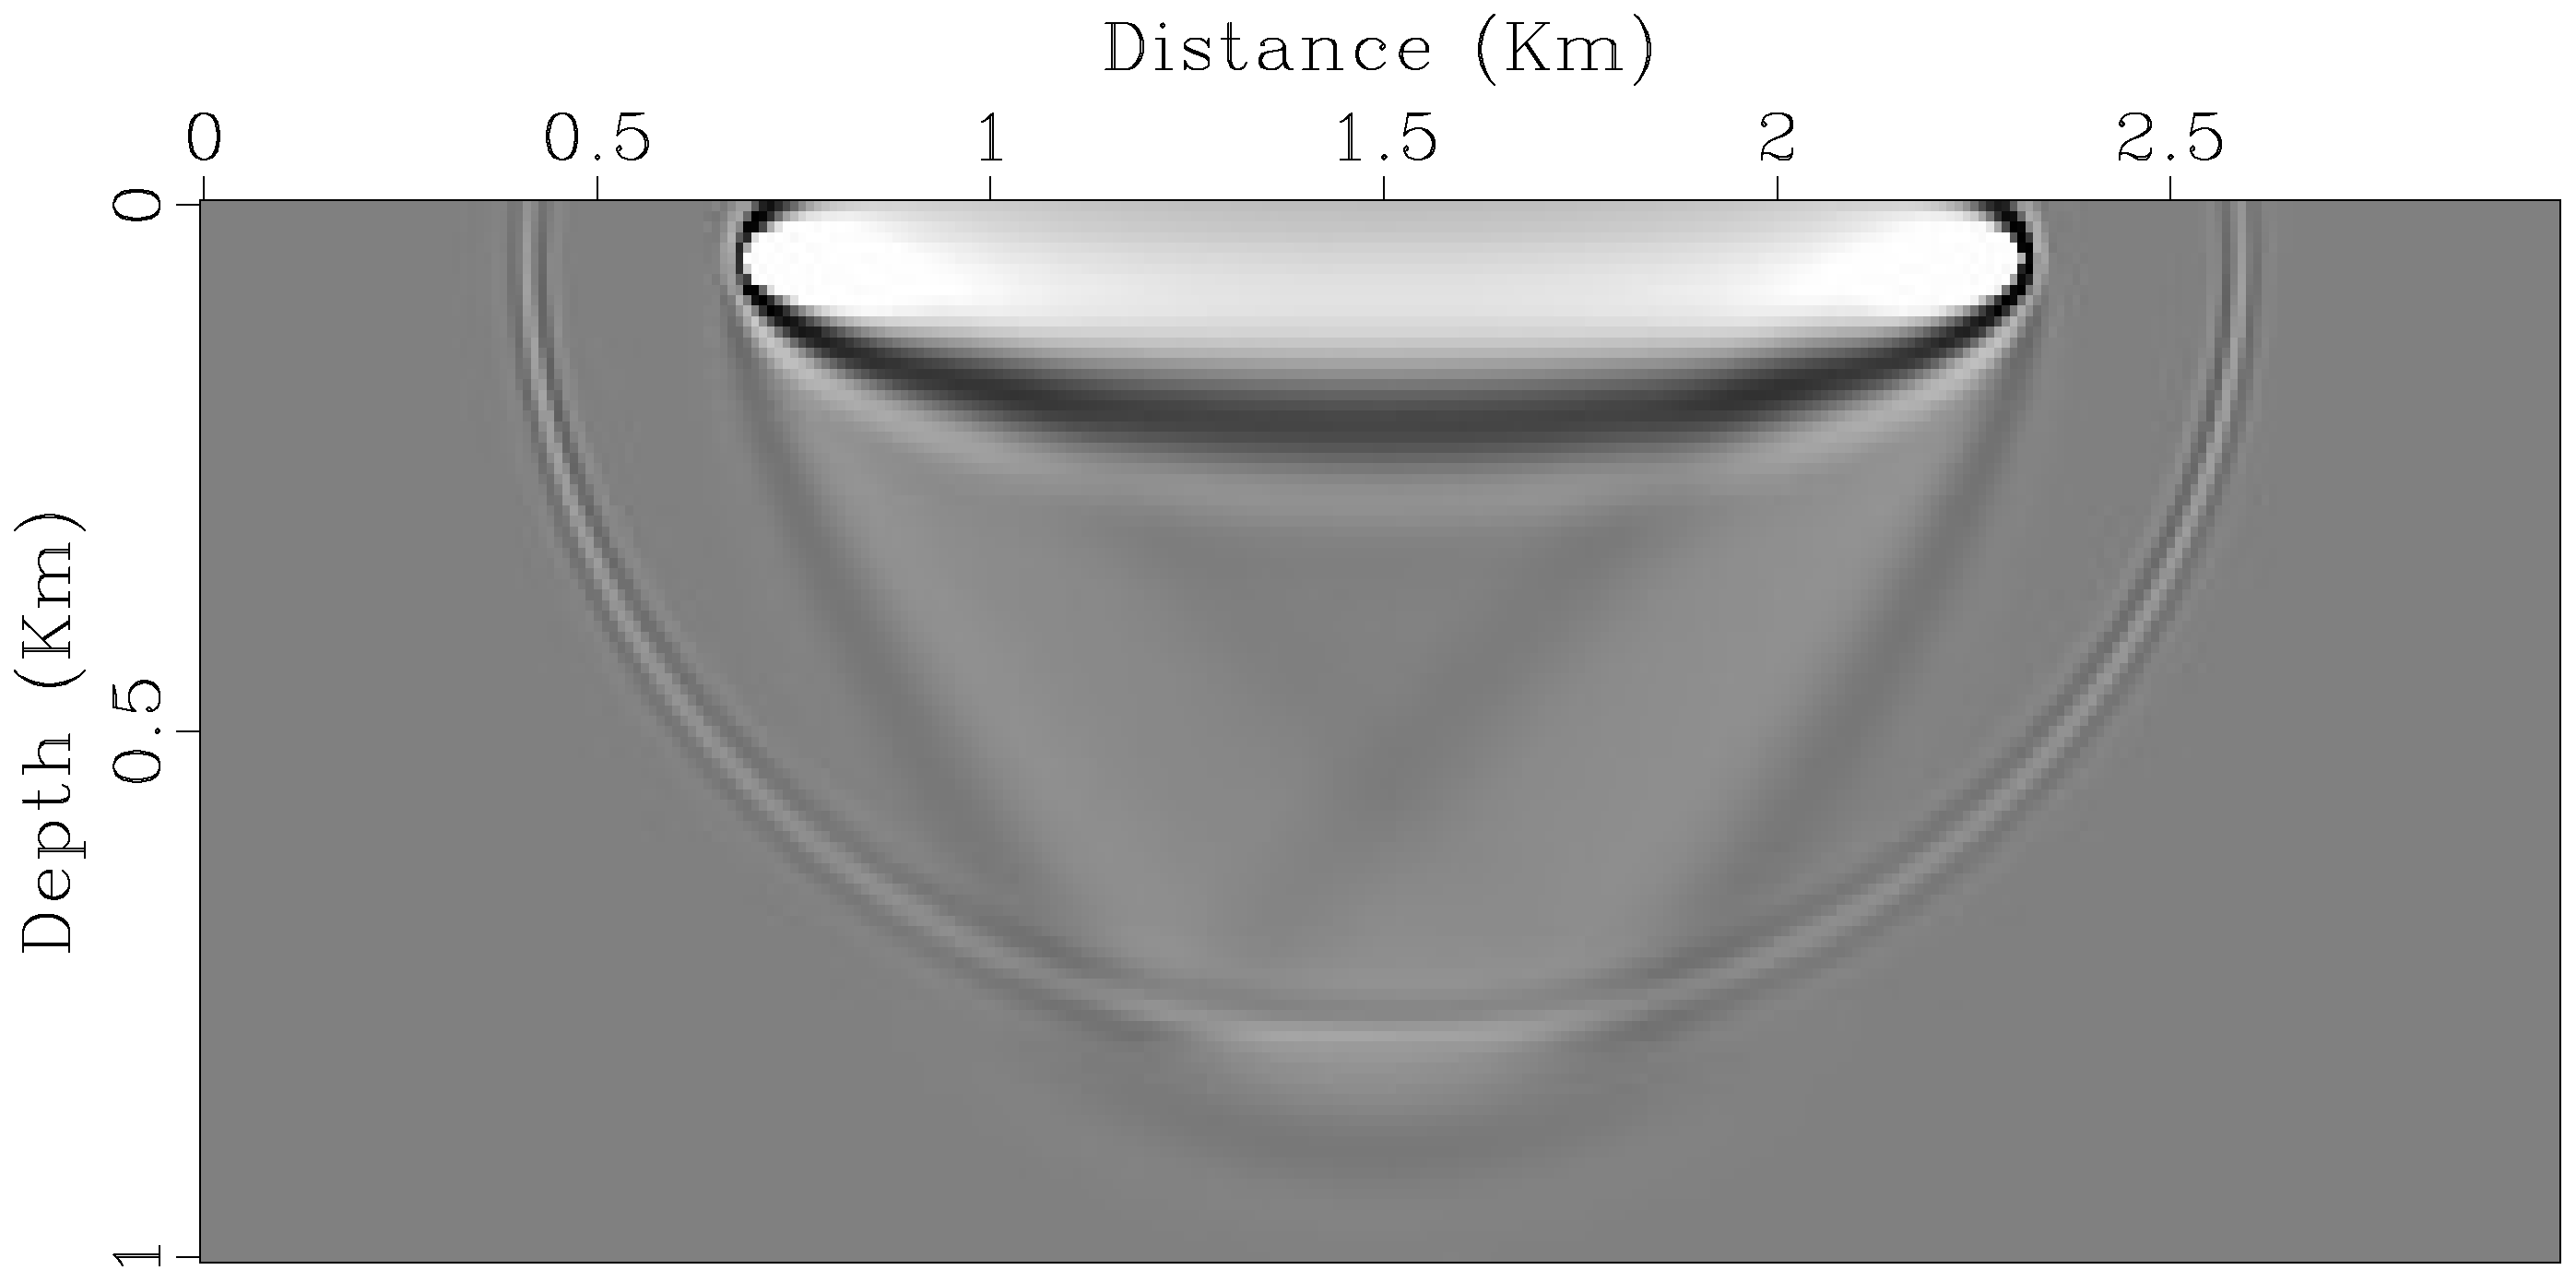
\includegraphics[width=0.95\linewidth]{figure/grad_full}
	\fcaption{两层介质单炮单检波点的FWI梯度。}{The gradient of FWI.
	 }[常规FWI梯度]
	\label{fig:grad_full}
\end{figure*}

\begin{figure*}[!htbp]
	\centering
	\subfigure[]{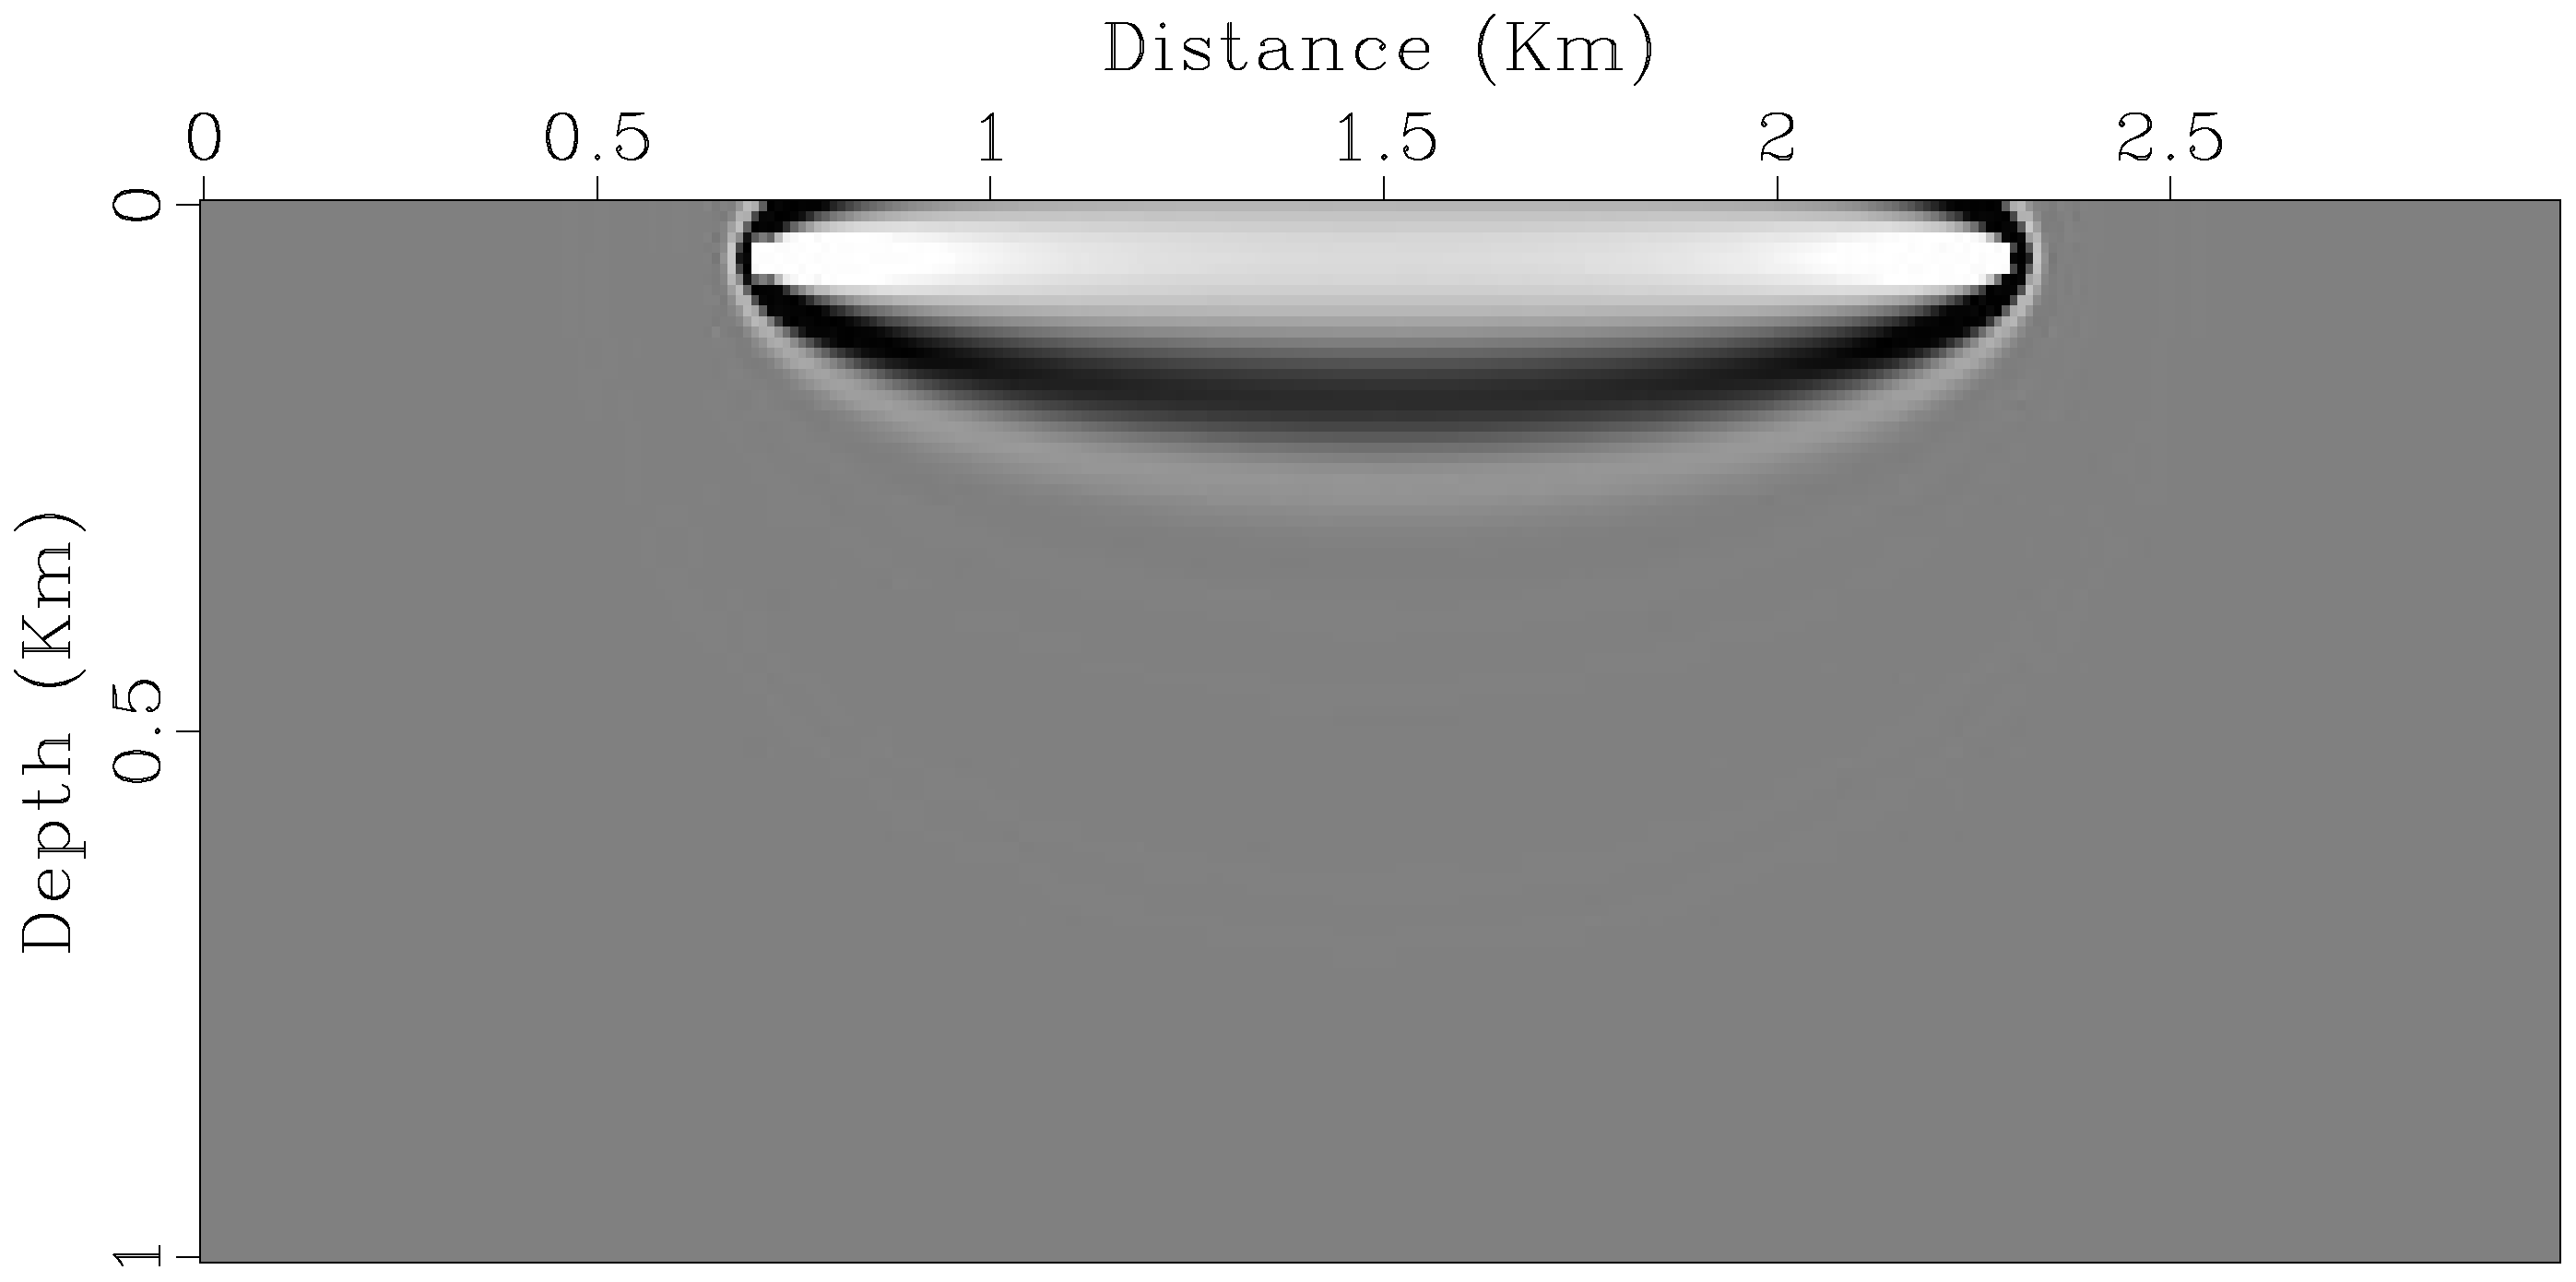
\includegraphics[width=0.45\linewidth]{figure/grad_fwi_dir}}
	\subfigure[]{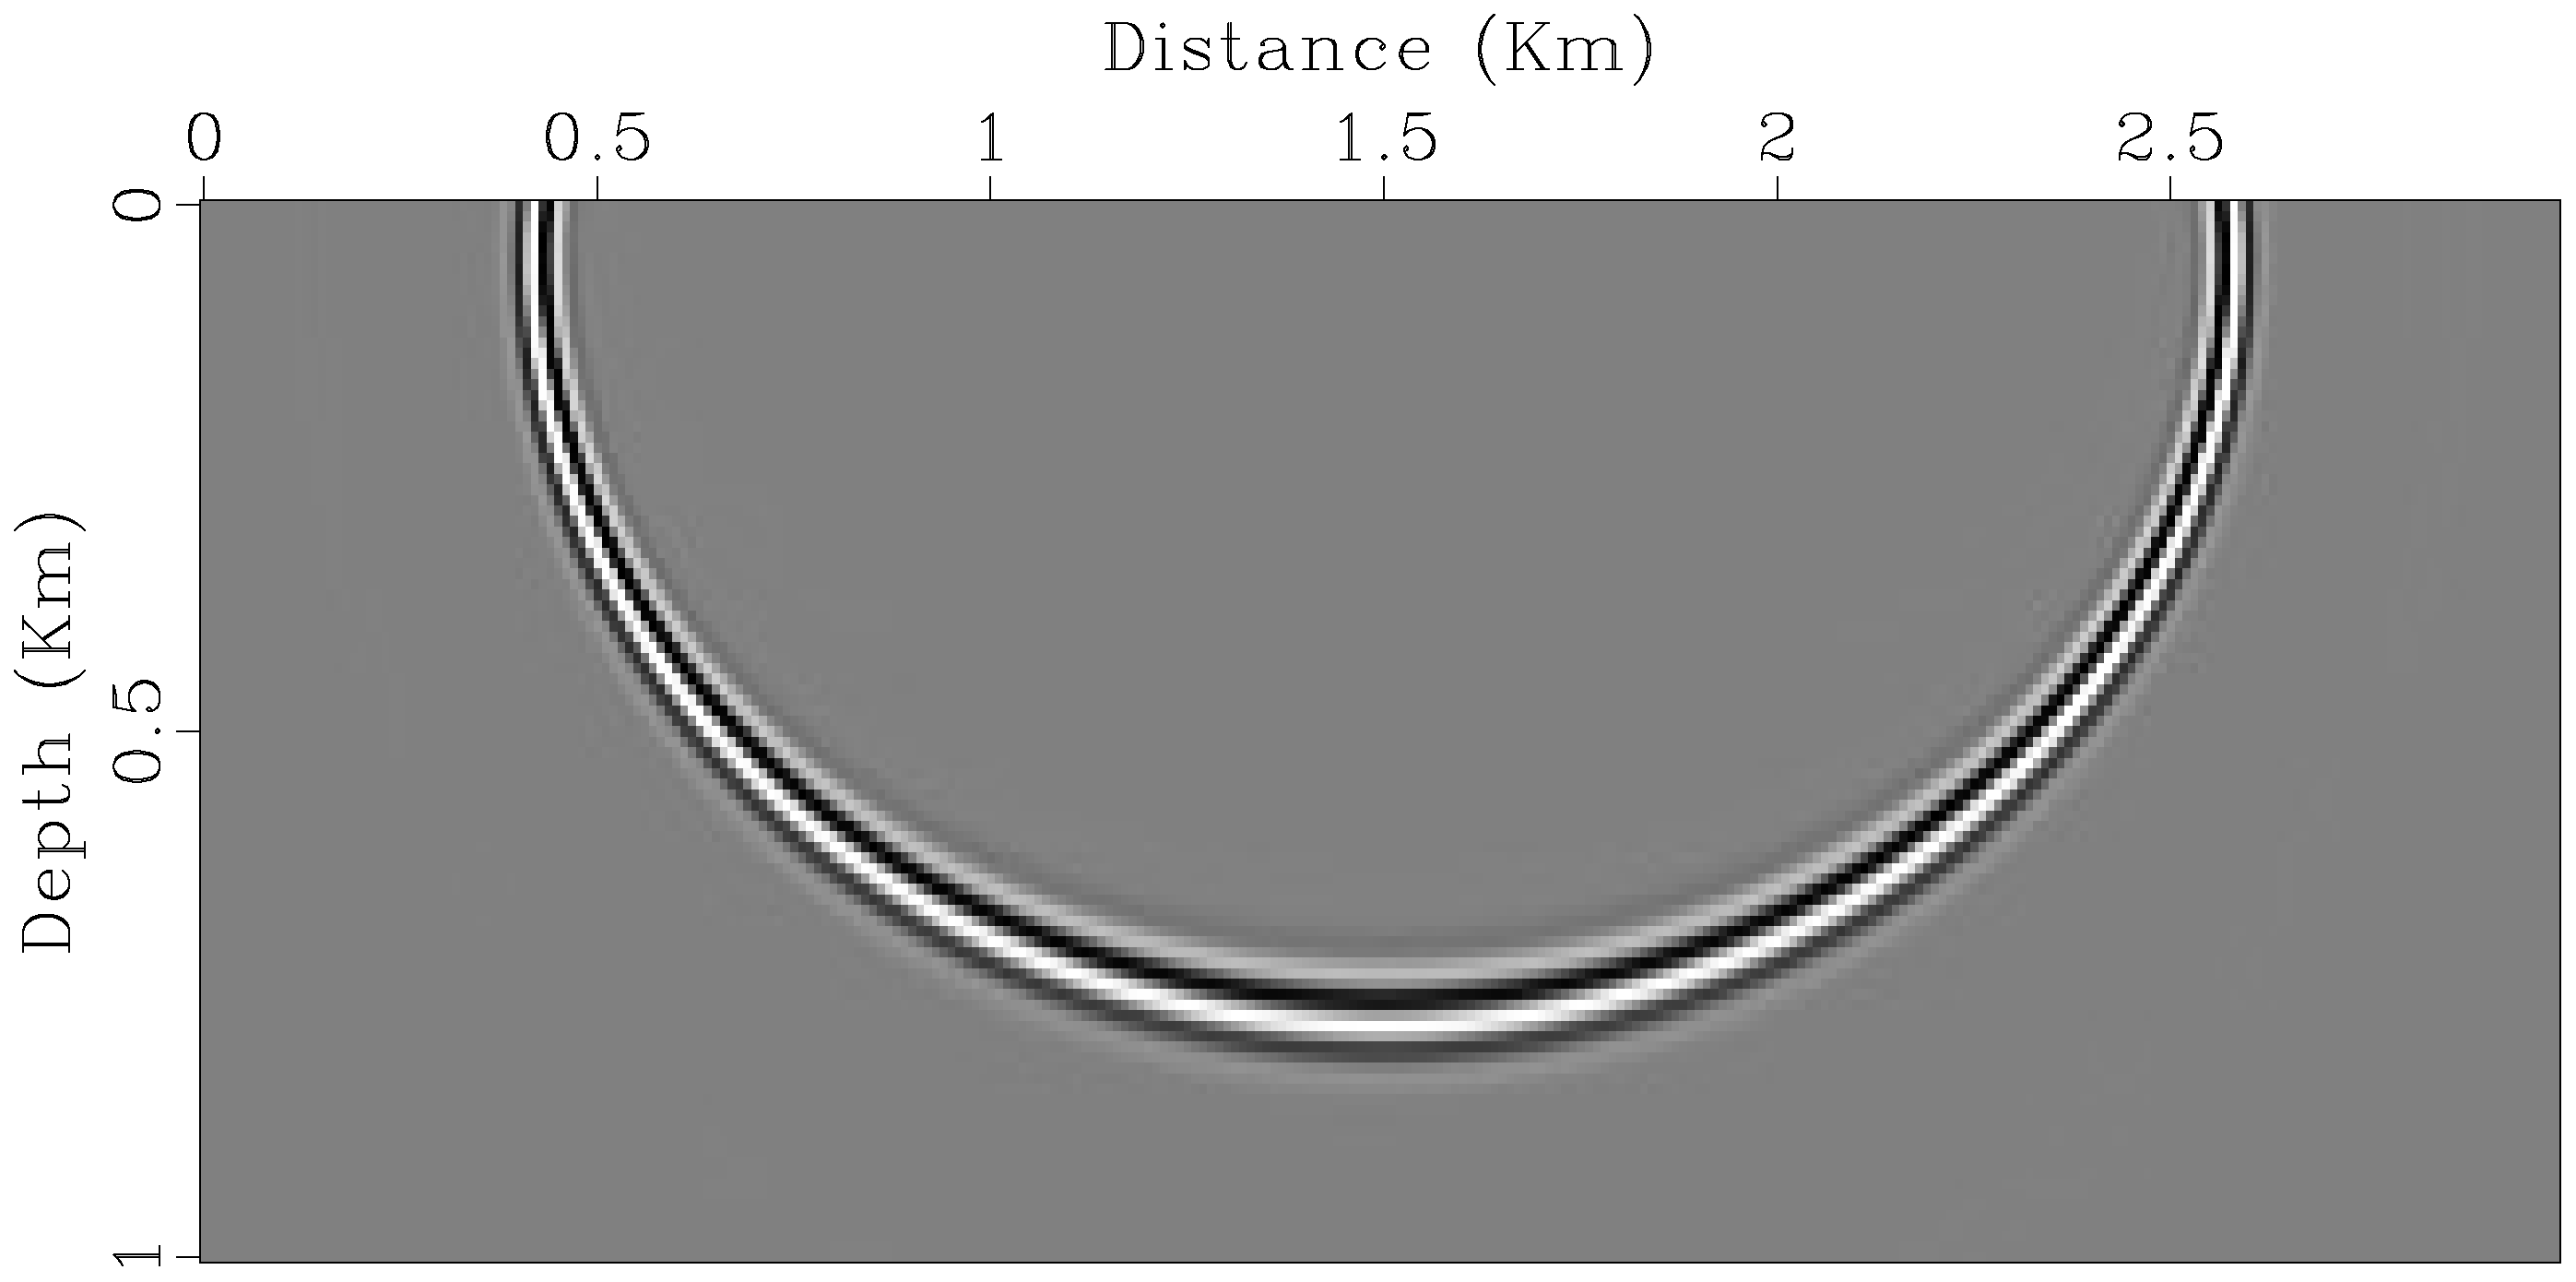
\includegraphics[width=0.45\linewidth]{figure/grad_mig}}
	\subfigure[]{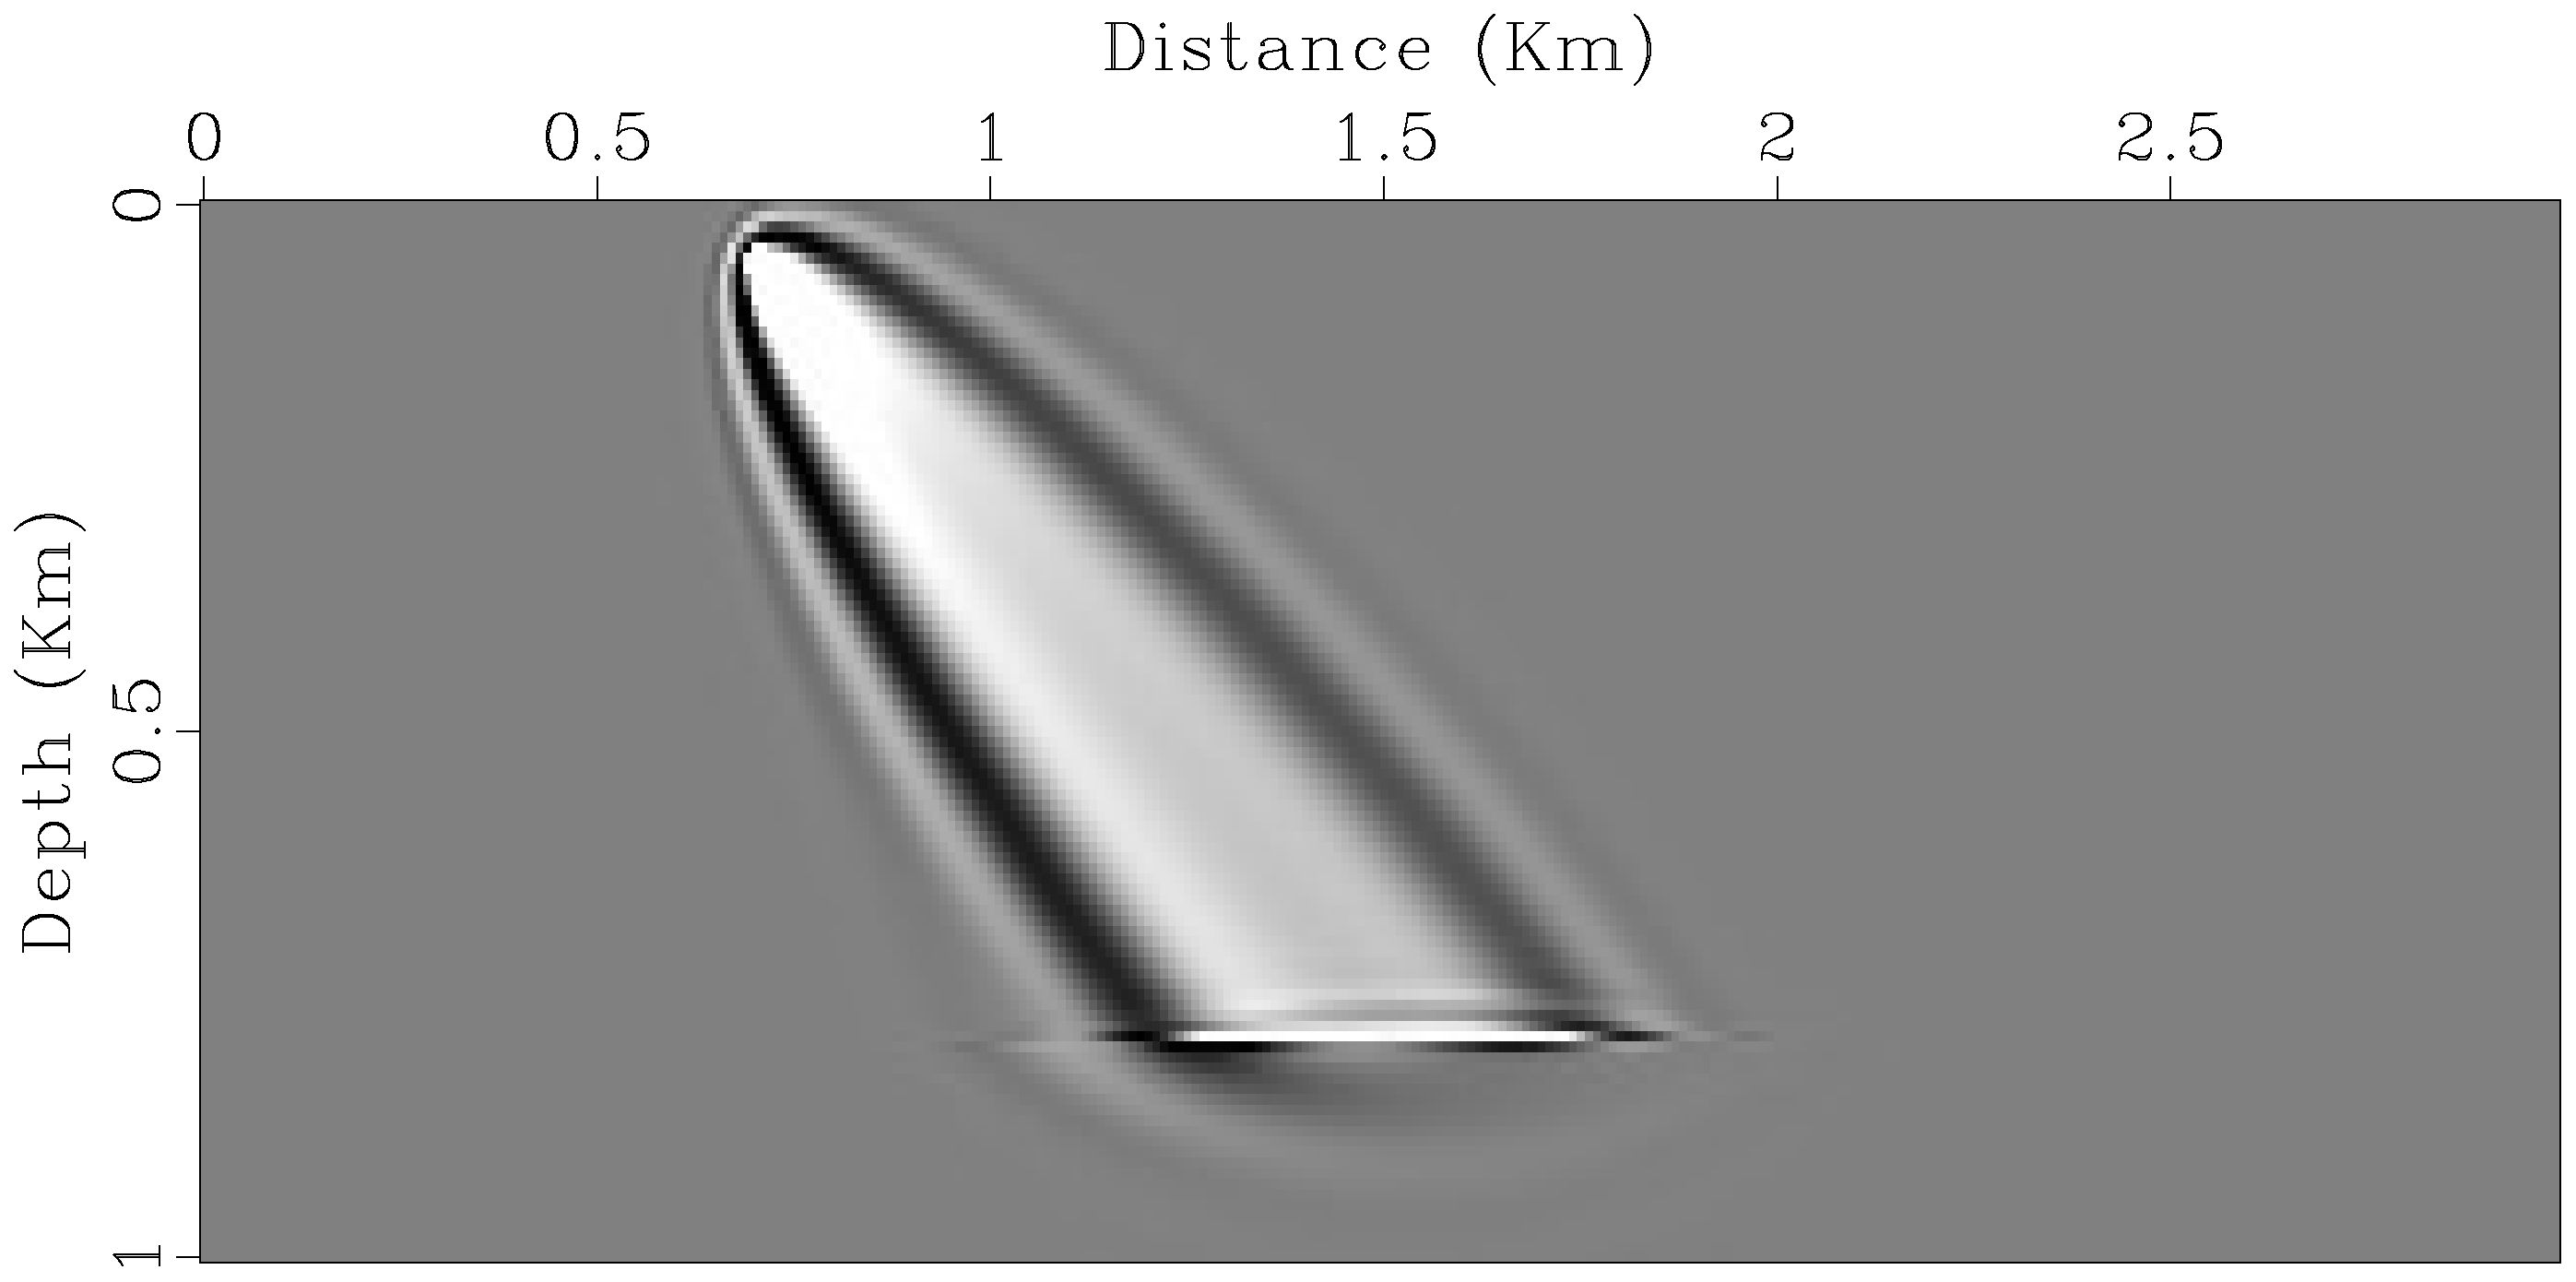
\includegraphics[width=0.45\linewidth]{figure/grads_rwi_one}}
	\subfigure[]{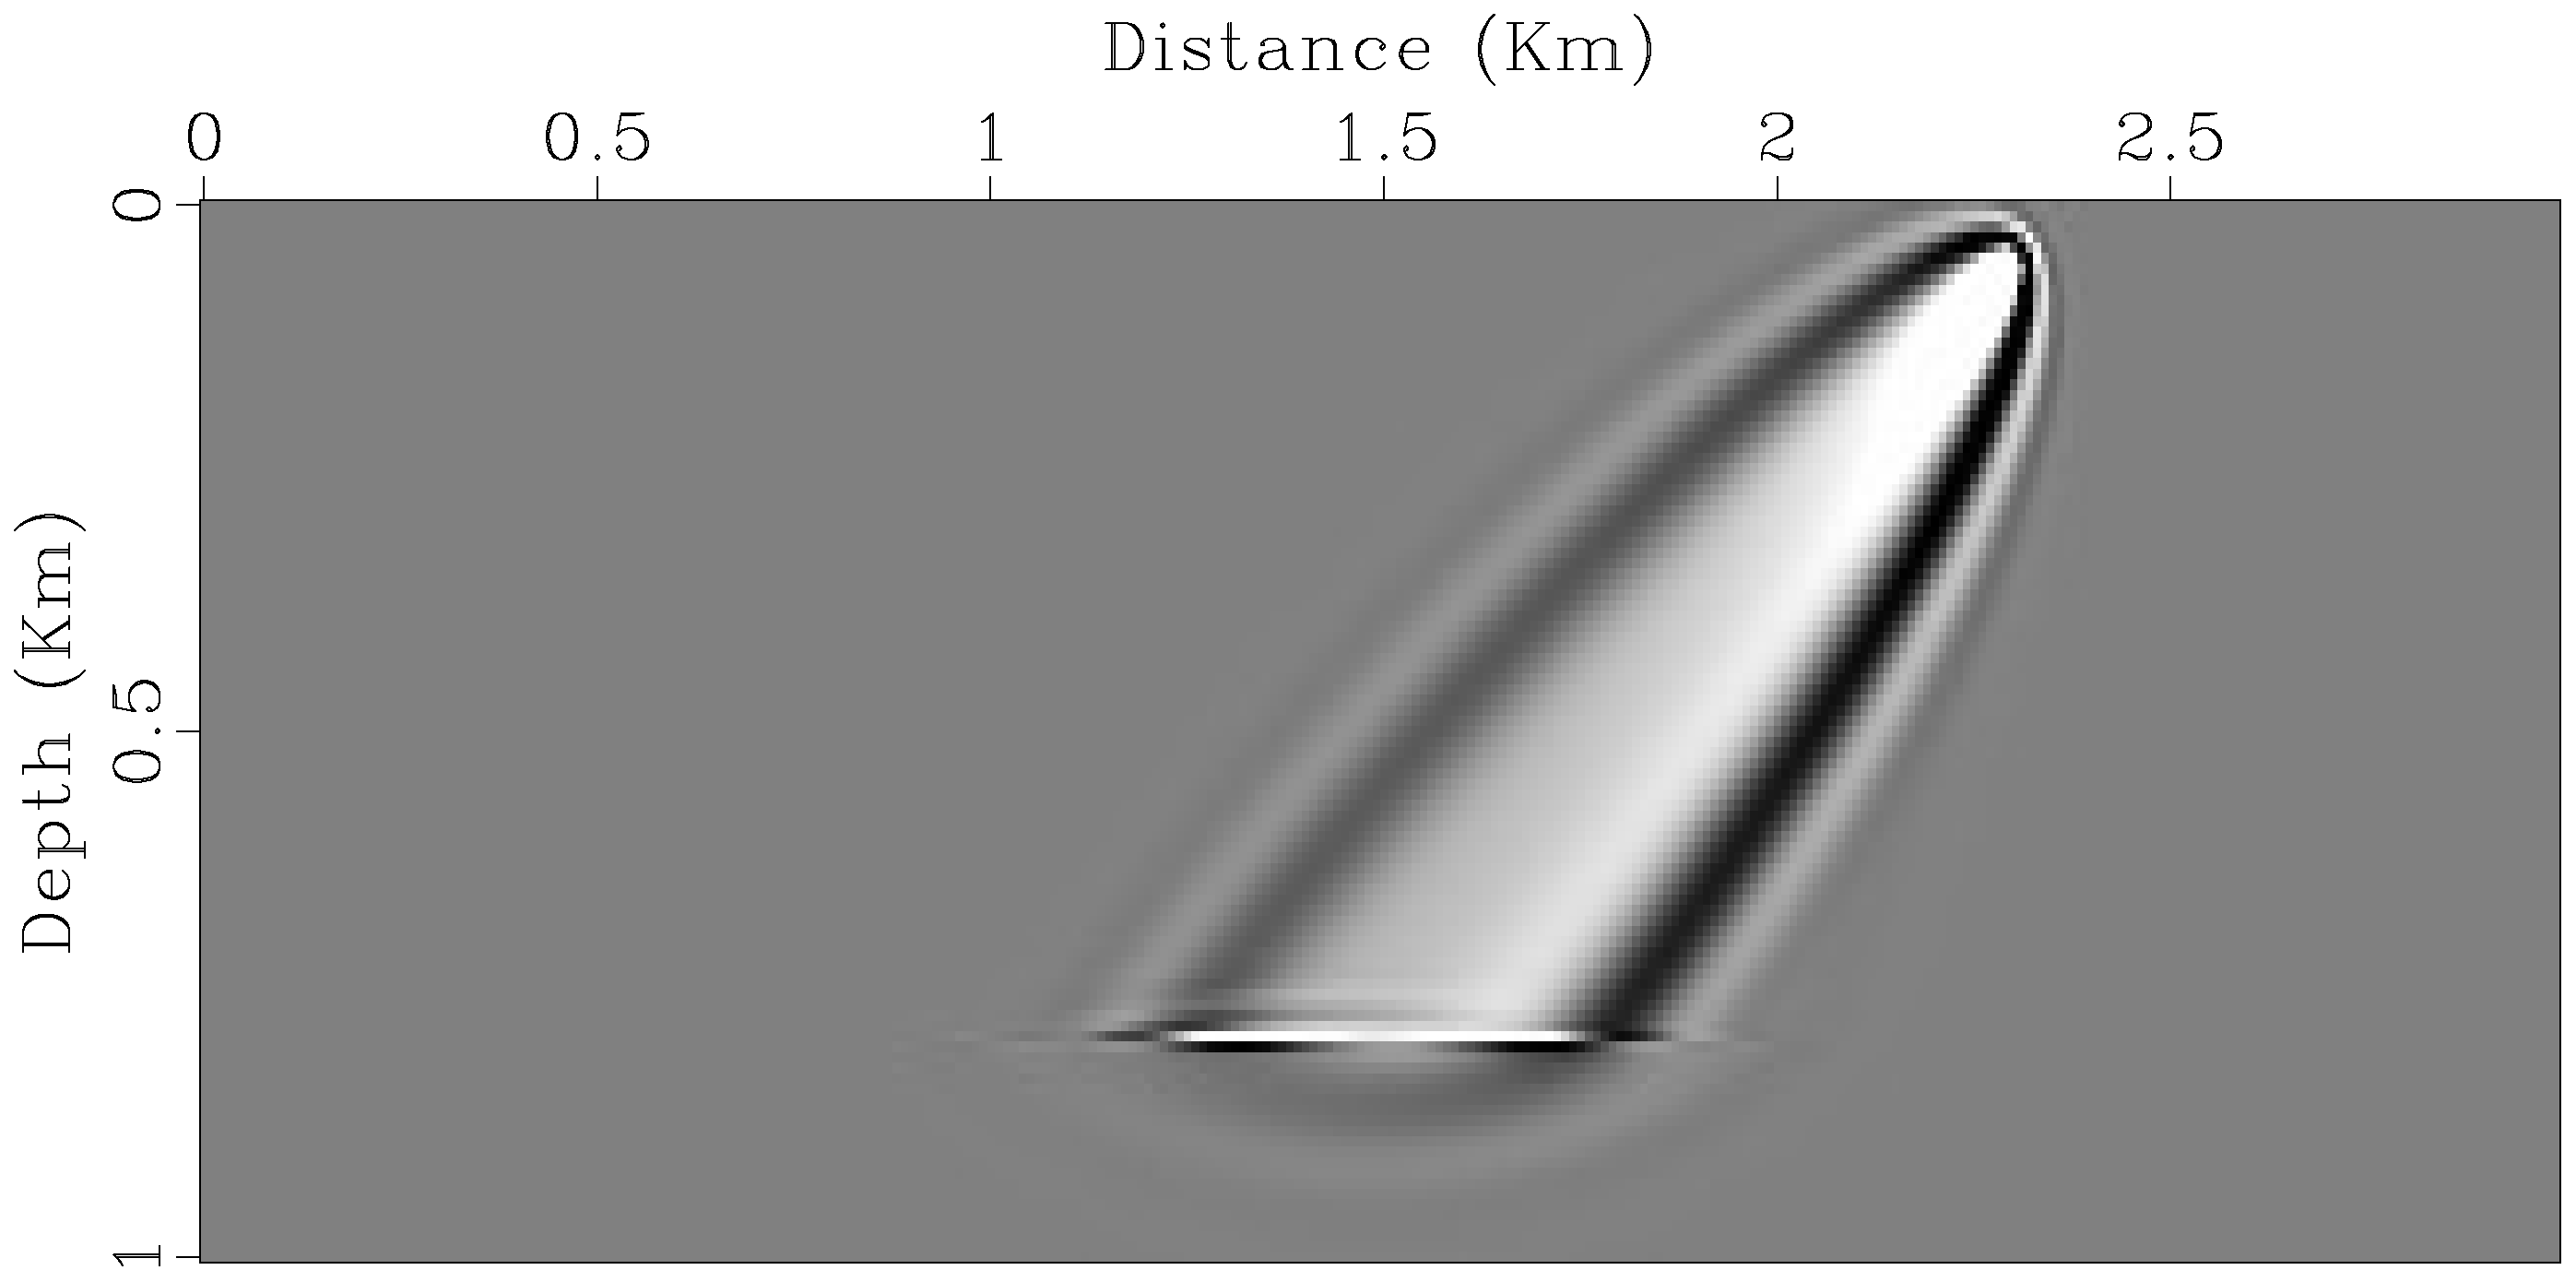
\includegraphics[width=0.45\linewidth]{figure/gradr_rwi_one}}
	\fcaption{常规FWI梯度分解。(a)直达波梯度;(b)偏移响应;(c)源端反射波梯度;
	(d)检波点端反射波梯度。}{The sub-gradients of FWI. (a) direct wave gradient; 
	(b) migration-ellipse; (c) source side gradient; (d) receiver side gradient.
	 }[常规FWI梯度分解]
	\label{fig:grad}
\end{figure*}

RWI主要是通过上下行波分离来提取反射波在反射波路径上的梯度。目前在RWI中用于上下行波分离
的方法主要两种,一种是在光滑的背景模型中加入参数扰动,用Born正演来获取上行的反射波
(\citeA{xu:2012a};\citeA{ma.hale:2013};\citeA{chi:2015});另一种是在频率-波数域
用方向分解来区分上下行波(\citeA{wang:2016})。另外,单成波方程自然地考虑了波的传播
方向,非常适合RWI的框架,已逐渐开始被学者用于RWI的研究中(\citeA{dong:2018})。
本节将用基于Born正演的方式来重述RWI的推导。

根据\citeB{ma.hale:2013}的推导,将模型参数$\mathbf{m}$分解为光滑的低波数背景模型
$\mathbf{m}^s$和高波数扰动$\mathbf{m}^r$(图~\ref{fig:schematic_rwi}):
\begin{equation}
	\mathbf{m}=\mathbf{m}^s+\mathbf{m}^r.
\end{equation}
其中光滑的背景参数$\mathbf{m}^s$控制波传播的运动学信息,即背景波场$\mathbf{p}_b
\equiv p_b(\mathbf{x}_s,\mathbf{x}_g,t)$:
\begin{equation}
	\left(\mathbf{m}^s\frac{\partial^2}{\partial t^2}-\bigtriangledown^2\right)\mathbf{p}_b
	=f(t,\mathbf{x}_s),
\end{equation}
高波数扰动$\mathbf{m}^r$对应于反射波场$\mathbf{p}_c\equiv p_c(\mathbf{x}_s,\mathbf{x}_g,t)$:
\begin{equation}
	\left((\mathbf{m}^s+\mathbf{m}^r)\frac{\partial^2}{\partial t^2}-\bigtriangledown^2\right)
	\mathbf{p}_c=-\mathbf{m}^r\frac{\partial^2}{\partial t^2}\mathbf{p}_b,
\end{equation}
式中$\mathbf{m}^r$和$\mathbf{m}^s$是慢度的平方,$f(t,\mathbf{x}_s)$表示震源子波。

\begin{figure*}[!htbp]
	\centering
	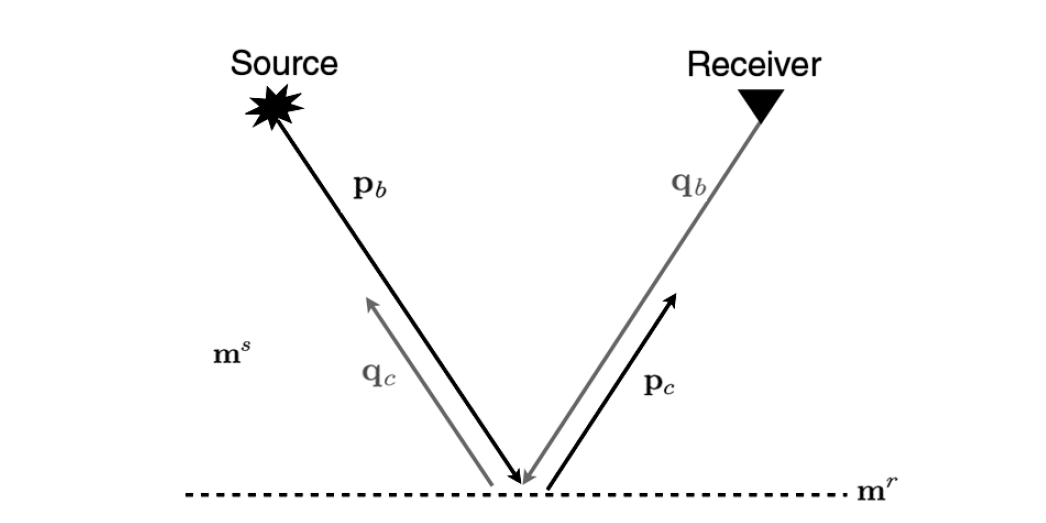
\includegraphics[width=0.7\linewidth]{figure/schematic_rwi}
	\fcaption{RWI波场分解及波路径示意图,参数的高波数成分($\mathbf{m}^r$)扰动背景场
	$\mathbf{p}_b$和$\mathbf{q}_b$产生背向散射场$\mathbf{p}_c$和$\mathbf{q}_c$,可以看作
	是”透射波“从震源出发沿波路径到达反射位置$\mathbf{m}^r$然后再返回接收点。}
	{Schematic of RWI. The high-wavenumber component
	$m^r$ perturbs wavefields $\mathbf{p}_b$ and $\mathbf{q}_b$ in the
	low-wavenumber background $m^s$ and contributes to back-scattering
	wavefields $\mathbf{p}_c$ and $\mathbf{q}_c$, which can be considered
	“transmission” waves propagating along the wave paths between $m^r$ and
	the source and receiver.}[RWI波场分解及波路径示意图]
	\label{fig:schematic_rwi}
\end{figure*}

根据伴随状态法(\citeA{plessix:2006}),低波数背景模型的梯度可以表示为(\citeA{ma.hale:2013}):
\begin{equation}
	\partial_{\mathbf{m}^s}\mathcal{J}=-\int d\mathbf{x}_sdt\mathbf{q}_c\ddot{\mathbf{p}}_b
	-\int d\mathbf{x}_sdt\mathbf{q}_b\ddot{\mathbf{p}}_c,
	\label{eq:grad_ms}
\end{equation}
高波数的扰动模型的梯度为:
\begin{equation}
	\partial_{\mathbf{m}^r}\mathcal{J}=-\int d\mathbf{x}_sdt\mathbf{q}_b\ddot{\mathbf{p}}_b
\end{equation}
式中$\mathbf{q}_b\equiv q_b(\mathbf{x}_s,\mathbf{x}_g,t)$和
$\mathbf{q}_c\equiv q_c(\mathbf{x}_s,\mathbf{x}_g,t)$是伴随场,即伴随方程的解。
方程~\ref{eq:grad_ms}右端的第一项表示源端的正传波场$\ddot{\mathbf{p}}_b$与反传波场
$\mathbf{q}_c$的零延迟互相关(图~\ref{fig:grad}c),同样地,第二项是正传波场$\ddot{\mathbf{p}}_c$和检波点端
反传波场$\mathbf{q}_b$的零延迟互相关(图~\ref{fig:grad}d)。正如图~\ref{fig:schematic_rwi}所示,模型的高波数
成分$\mathbf{m}^r$散射源端的正传背景场$\mathbf{p}_b$和检波点端的反传背景场$\mathbf{q}_b$,
换句话说,$\mathbf{m}^r$中的每一点都可以看成是虚拟震源来产生散射波场$\mathbf{p}_c$和
$\mathbf{q}_c$。背景模型的梯度$\partial_{\mathbf{m}^s}\mathcal{J}$跟预想的一样,是沿反射波的波路径分布的,
即从震源出发到达地下反射位置然后再返回接收点。这样的梯度携带了地下中深层的参数信息,用以更新中深层的背景
模型是可靠的。相反,$\partial_{\mathbf{m}^r}\mathcal{J}$类似于RTM成像结果,主要分布在反射
位置$\mathbf{m}^r$附近,用以产生反射数据。

\newpage
\subsection{基于粘声方程的反射全波形反演}
\vspace{0.5cm}

根据第二章第二节的推导,对于给定的速度以及$Q$模型,压力波场可用如下SLS方程进行计算:
     \begin{eqnarray}
        \begin{aligned}
        \frac{\partial P}{\partial t} -
        K(\tau+1)(\frac{\partial v_x}{\partial x}
        +\frac{\partial v_z}{\partial z})-r_p &=f(\mathbf{x}_s,t),
        \\
        \frac{\partial v_x}{\partial t} - \frac{1}{\rho}\frac{\partial P}{\partial x}
        &=0,\\
        \frac{\partial v_z}{\partial t} - \frac{1}{\rho}\frac{\partial P}{\partial z}&=0,\\
        \frac{\partial{r_p}}{\partial t} +
        \frac{1}{\tau_\sigma}\left[r_p+K\tau(\frac{\partial
        v_x}{\partial x}+\frac{\partial v_z}{\partial z})\right]&=0,
        \end{aligned}
        \label{eq:viscoacoustic}
    \end{eqnarray}
式中$v_x$和$v_z$表示质点的振动速度,$P$表示压力场,$r_p$为记忆变量,$K$表示介质的体积
模量,为了简化表示我们假定密度是常数。应力以及应变的驰豫参数$\tau_\sigma$,$\tau_\epsilon$
以及$\tau$与品质因子$Q$和参考频率$f_\omega$有关,在地震勘探应用中,通常选取震源子波
的中心频率为其参考频率,即有:
    \begin{eqnarray}
        \begin{aligned}
            \tau_\sigma &= \frac{\sqrt{1+\frac{1}{Q^2}}-\frac{1}{Q}}{f_\omega},\\
            \tau_\epsilon &= \frac{1}{f^2_\omega\tau_\sigma}=\frac{\sqrt{1+\frac{1}{Q^2}}+\frac{1}{Q}}{f_\omega},
        \end{aligned}
    \end{eqnarray}
以及
    \begin{eqnarray}
        \tau=\frac{\tau_\epsilon}{\tau_\sigma}-1=\frac{2}{Q}(\frac{1}{Q}+\sqrt{1+\frac{1}{Q^2}}).
        \label{eq:tq}
    \end{eqnarray}

在$Q$-RWI中,主要反演背景的$Q$,我们认为衰减对宏观地震波的影响主要发生在波路径上,
即是一种传播效应不是界面效应,所以不对$Q$进行波数成分的分解。为了描述波路径产生反射波,携带
衰减信息,我们将体积模量$K$分解为光滑背景$K_0$和高波数扰动$\delta K$:
\begin{equation}
	K = K_0 + \delta K.
\end{equation}
根据SLS粘声波方程~\ref{eq:viscoacoustic}以及Born近似假设,$Q$-RWI的物理状态方程可
写为如下矩阵向量乘的形式:
\begin{equation}
    \mathbf{L}\mathbf{w} = \mathbf{f},
    \label{eq:state}
\end{equation}
其中
    \begin{eqnarray*}
        \mathbf{L}= 
        \begin{bmatrix}
            \begin{smallmatrix}
            \frac{\partial}{\partial t} &-K_0(\tau +1)\frac{\partial}{\partial x}
            &-K_0(\tau +1)\frac{\partial}{\partial z} &-1 &0 &0 &0 &0\cr
            -\frac{1}{\rho}\frac{\partial}{\partial x} &\frac{\partial}{\partial t} &0
            &0 &0 &0 &0 &0\cr
            -\frac{1}{\rho}\frac{\partial}{\partial z} &0 &\frac{\partial}{\partial t}
            &0 &0 &0 &0 &0\cr
            0 & \frac{\tau}{\tau_\sigma}K_0\frac{\partial}{\partial x}
            &\frac{\tau}{\tau_\sigma}K_0\frac{\partial}{\partial z}
            &\frac{\partial}{\partial t}+\frac{1}{\tau_\sigma} &0 &0 &0 &0 \cr
            0 &-\delta K(\tau+1)\frac{\partial}{\partial x} &-\delta
            K(\tau+1)\frac{\partial}{\partial z} &0 &\frac{\partial}{\partial t}
            &-K_0(\tau +1)\frac{\partial}{\partial x} &-K_0(\tau
            +1)\frac{\partial}{\partial z} &-1 \cr
            0 &0 &0 &0 &-\frac{1}{\rho}\frac{\partial}{\partial x}
            &\frac{\partial}{\partial t} &0 &0\cr
            0 &0 &0 &0 &-\frac{1}{\rho}\frac{\partial}{\partial z} &0
            &\frac{\partial}{\partial t} &0\cr
            0 &\frac{\tau}{\tau_\sigma}\delta K\frac{\partial}{\partial x}
            &\frac{\tau}{\tau_\sigma}\delta K\frac{\partial}{\partial z} &0 &0 
            & \frac{\tau}{\tau_\sigma}K_0\frac{\partial}{\partial x}
            &\frac{\tau}{\tau_\sigma}K_0\frac{\partial}{\partial z}
            &\frac{\partial}{\partial t}+\frac{1}{\tau_\sigma}
            \end{smallmatrix}
        \end{bmatrix}
    \end{eqnarray*}
以及
    \begin{eqnarray*}
        \mathbf{w} = 
        \begin{bmatrix}
            P \cr v_x \cr v_z \cr r_p \cr\delta P \cr\delta v_x \cr\delta v_z
            \cr\delta r_p
        \end{bmatrix},
        \mathbf{f} = 
        \begin{bmatrix}
            f \cr 0\cr 0\cr 0 \cr 0\cr 0 \cr 0\cr 0
        \end{bmatrix}.
    \end{eqnarray*}
$\mathbf{w}$表示状态变量,$\mathbf{L}$表示正演模拟算子。在这种情况下,
正算子的伴随算子$\mathbf{L}^\ast$有如下表达式:
    \begin{eqnarray}
        \mathbf{L}^\ast =  
        \begin{bmatrix}
            \begin{smallmatrix}
            -\frac{\partial}{\partial t} &\frac{\partial}{\partial x}\frac{1}{\rho}
            &\frac{\partial}{\partial z}\frac{1}{\rho} &0 &0 &0 &0 &0\cr
            \frac{\partial}{\partial x}K_0(\tau +1) &-\frac{\partial}{\partial t} &0 
            &-\frac{\partial}{\partial x}\frac{\tau}{\tau_\sigma}K_0
            &\frac{\partial}{\partial x}\delta K(\tau+1) &0 &0
            &-\frac{\partial}{\partial x}\frac{\tau}{\tau_\sigma}\delta K \cr
            \frac{\partial}{\partial z}K_0(\tau +1) &0 &-\frac{\partial}{\partial t} 
            &-\frac{\partial}{\partial z}\frac{\tau}{\tau_\sigma}K_0
            &\frac{\partial}{\partial z}\delta K(\tau+1) &0 &0
            &-\frac{\partial}{\partial z}\frac{\tau}{\tau_\sigma}\delta K \cr
            -1 &0 &0 &-\frac{\partial}{\partial t}+\frac{1}{\tau_\sigma} &0 &0 &0 &0\cr
            0 &0 &0 &0 &-\frac{\partial}{\partial t} &\frac{\partial}{\partial
            x}\frac{1}{\rho} &\frac{\partial}{\partial z}\frac{1}{\rho} &0\cr
            0 &0 &0 &0 &\frac{\partial}{\partial x}K_0(\tau +1)
            &-\frac{\partial}{\partial t} &0 &-\frac{\partial}{\partial
            x}\frac{\tau}{\tau_\sigma}K_0 \cr
            0 &0 &0 &0 &\frac{\partial}{\partial z}K_0(\tau +1) &0
            &-\frac{\partial}{\partial t} &-\frac{\partial}{\partial
        z}\frac{\tau}{\tau_\sigma}K_0 \cr
           0 &0 &0 &0 &-1 &0 &0 &-\frac{\partial}{\partial t}+\frac{1}{\tau_\sigma}
            \end{smallmatrix}
        \end{bmatrix},
		\label{eq:ad_operator}
    \end{eqnarray}
式中$\ast$表示伴随。对于真实的地质模型,驰豫参数$\tau$比$\tau_\sigma$和$\tau_\epsilon$
有较宽的数值变化范围。因此我们选择$\tau$作为参数化参数,因为其对$Q$的变化更敏感
(\citeA{dutta.schuster:2016})。用伴随状态法可推导出目标函数$\mathcal{J}(\mathbf{m})$
对驰豫参数$\tau$的梯度为:
   \begin{equation}
    \begin{aligned}
        \frac{\partial \mathcal{J}}{\partial \tau} &= -\langle\frac{\partial \mathbf{L}}{\partial\tau}
        \mathbf{w},\tilde{\mathbf{w}} \rangle \\
        &= {K_0(\frac{\partial v_x}{\partial
        x}+\frac{\partial v_z}{\partial
    z})(-\delta\tilde{P}+\frac{1}{\tau_\sigma}\delta\tilde{r}_p)} \\
    &{+K_0(\frac{\partial \delta v_x}{\partial x}+\frac{\partial \delta
        v_z}{\partial z})(-\tilde{P}+\frac{1}{\tau_\sigma}\tilde{r}_p)} \\
        &{+\delta K(\frac{\partial v_x}{\partial x}+\frac{\partial v_z}{\partial
        z})(-\tilde{P}+\frac{1}{\tau_\sigma}\tilde{r}_p)},
    \end{aligned}
    \label{eq:gradient}
    \end{equation}
式中$\tilde{\mathbf{w}}=\lbrack \delta\tilde{P}, \ \delta \tilde{v}_x, \ \delta \tilde{v}_z, \
\delta \tilde{r}_p, \ \tilde{P}, \ \tilde{v}_x, \ \tilde{v}_z, \ \tilde{r}_p\rbrack ^T$是
物理状态变量$\mathbf{w}$的伴随状态变量($T$表示转置),满足如下伴随方程:
\begin{equation}
	\mathbf{L}^\ast\tilde{\mathbf{w}} = \Delta\mathbf{d}.
\end{equation}
在实际勘探中,通常只接收到了波场的压力分量,所以地震数据的残差只有一个分量,即:
\begin{equation}
    \Delta\mathbf{d} = \lbrack 0, \ 0, \ 0, \ 0, \ \Delta d, \ 0, \ 0, \ 0\rbrack^T.
\end{equation}
本章主要是理论的角度来推导$Q$-RWI方法并证明其对反演深层背景衰减模型的有效性,所以我们
假定介质的背景体积模量$K_0$和扰动$\delta K$都是已知的,并且地震数据是无噪的。在这
中假设下选取振幅差作为目标函数(方程~\ref{eq:misfit_function})是可行的,并且伴随方程的
伴随源有最简单的形式即模拟数据与观测数据的残差。

\begin{figure*}[!htbp]
    \centering
    \subfigure[]{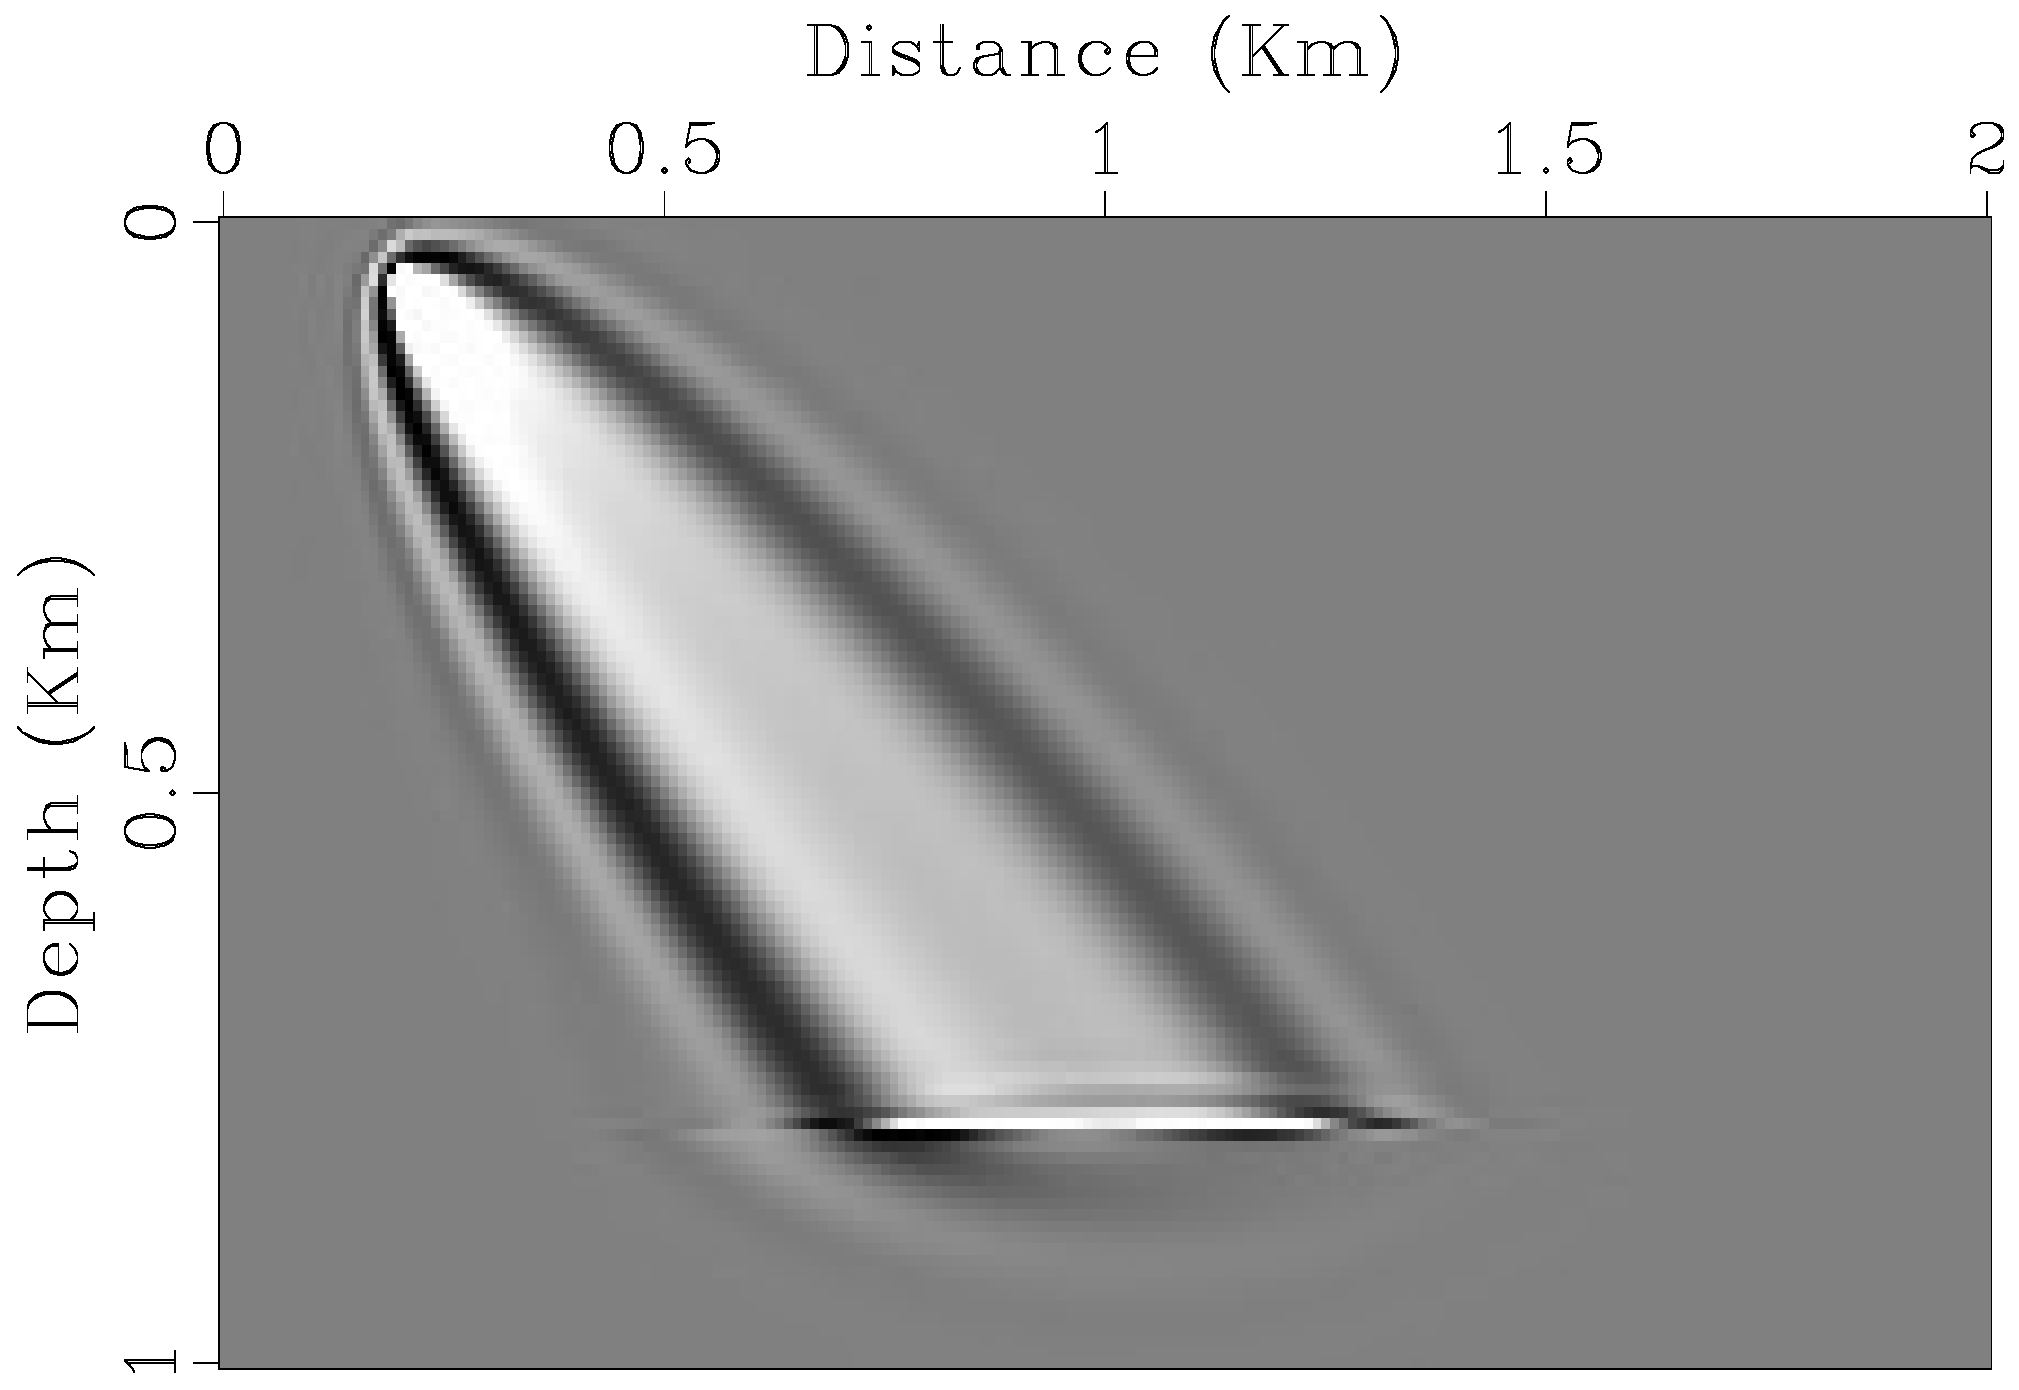
\includegraphics[width=0.45\linewidth]{figure/grad1}}
    \subfigure[]{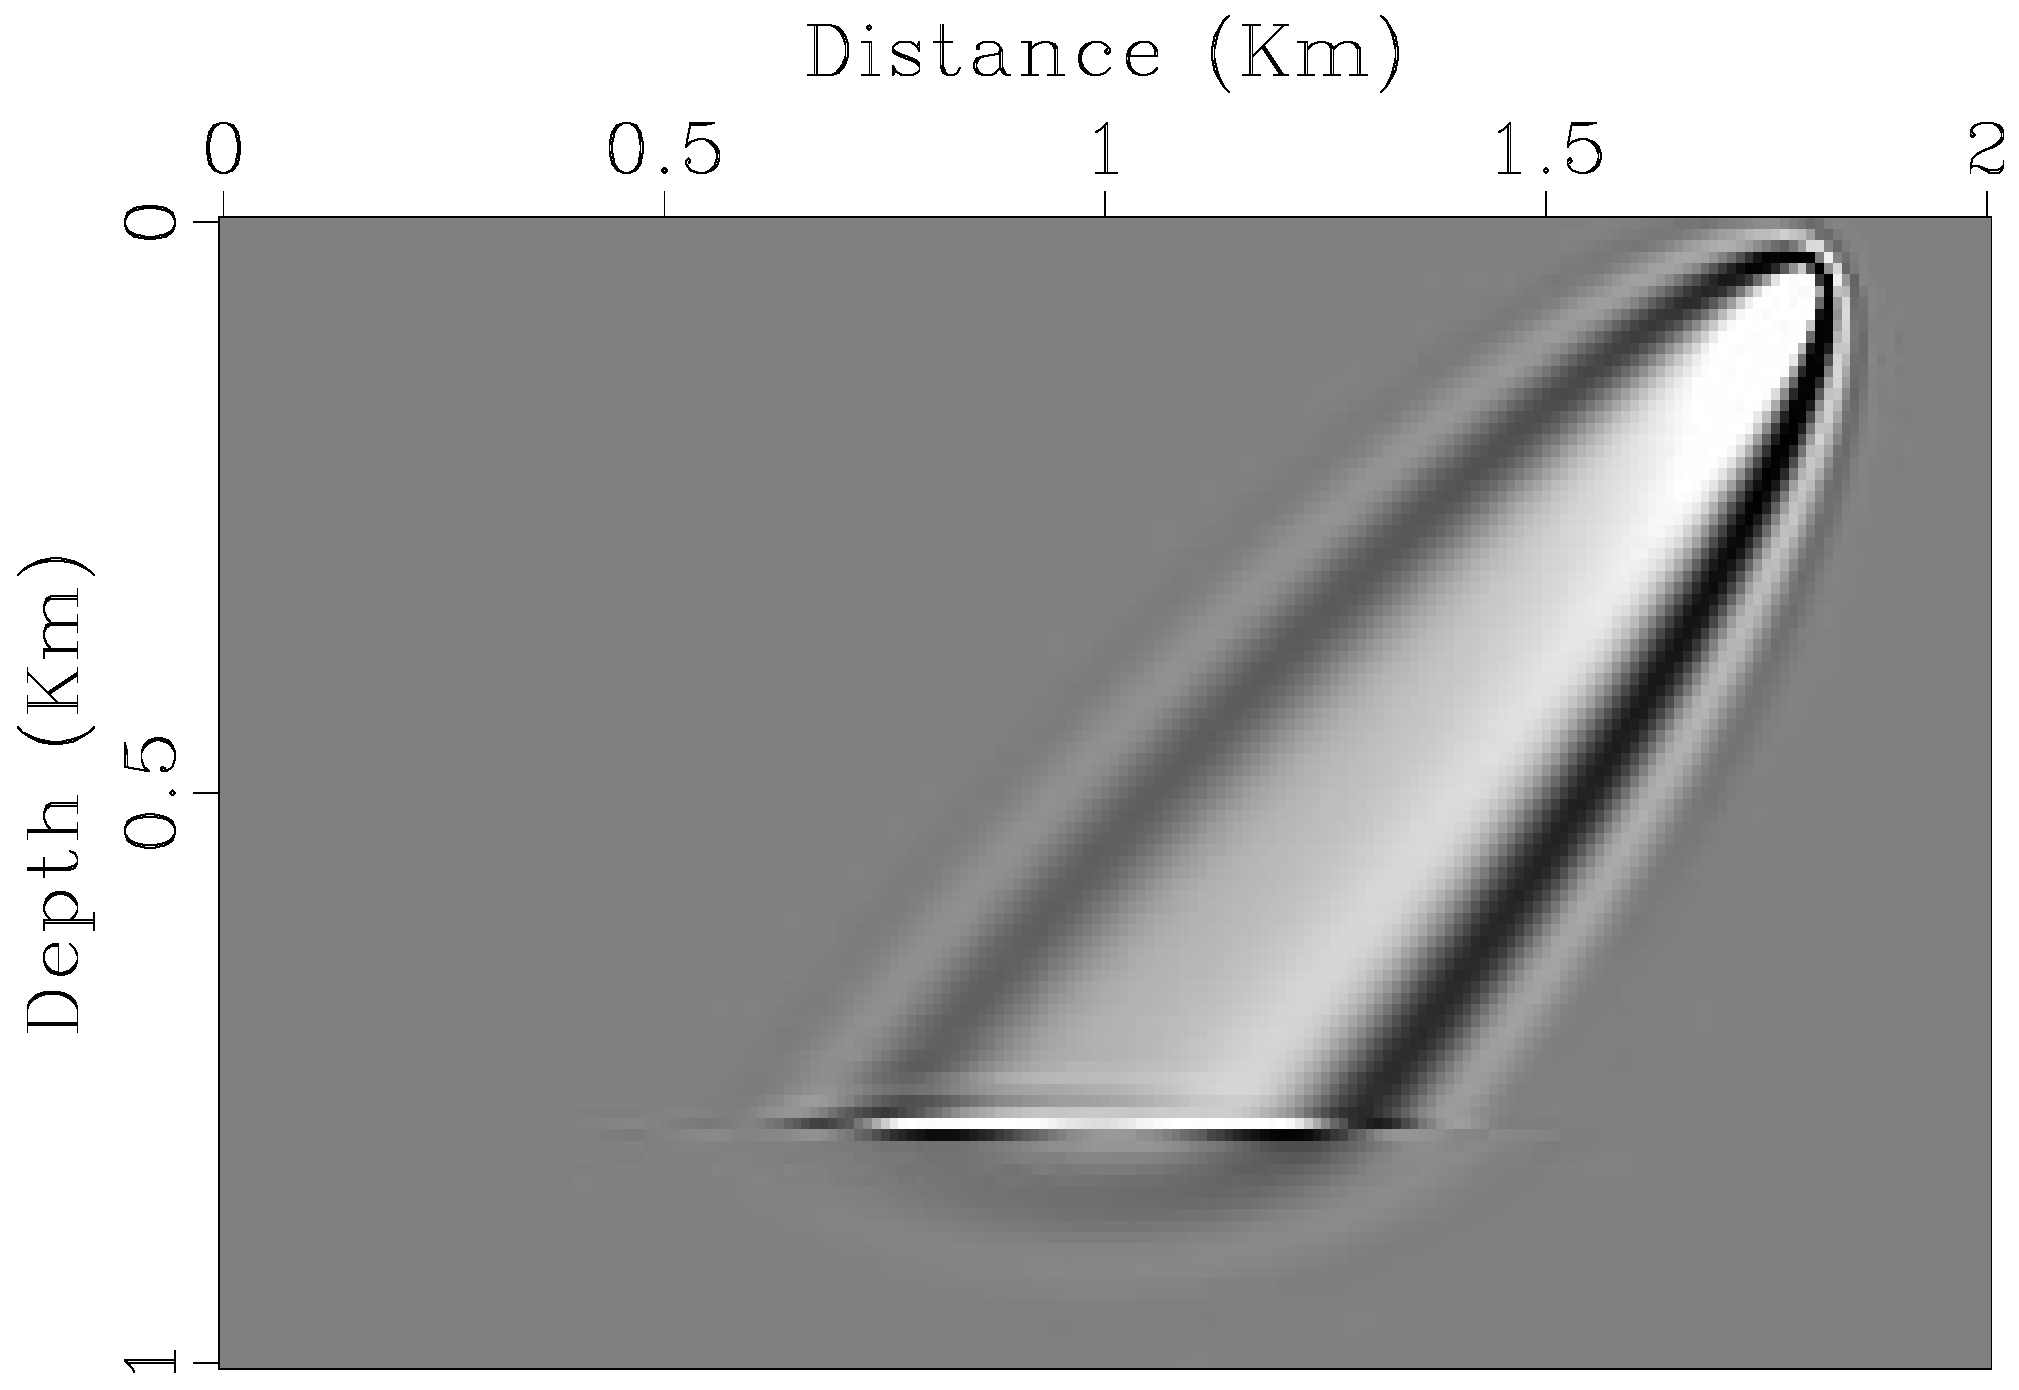
\includegraphics[width=0.45\linewidth]{figure/grad2}}
    \subfigure[]{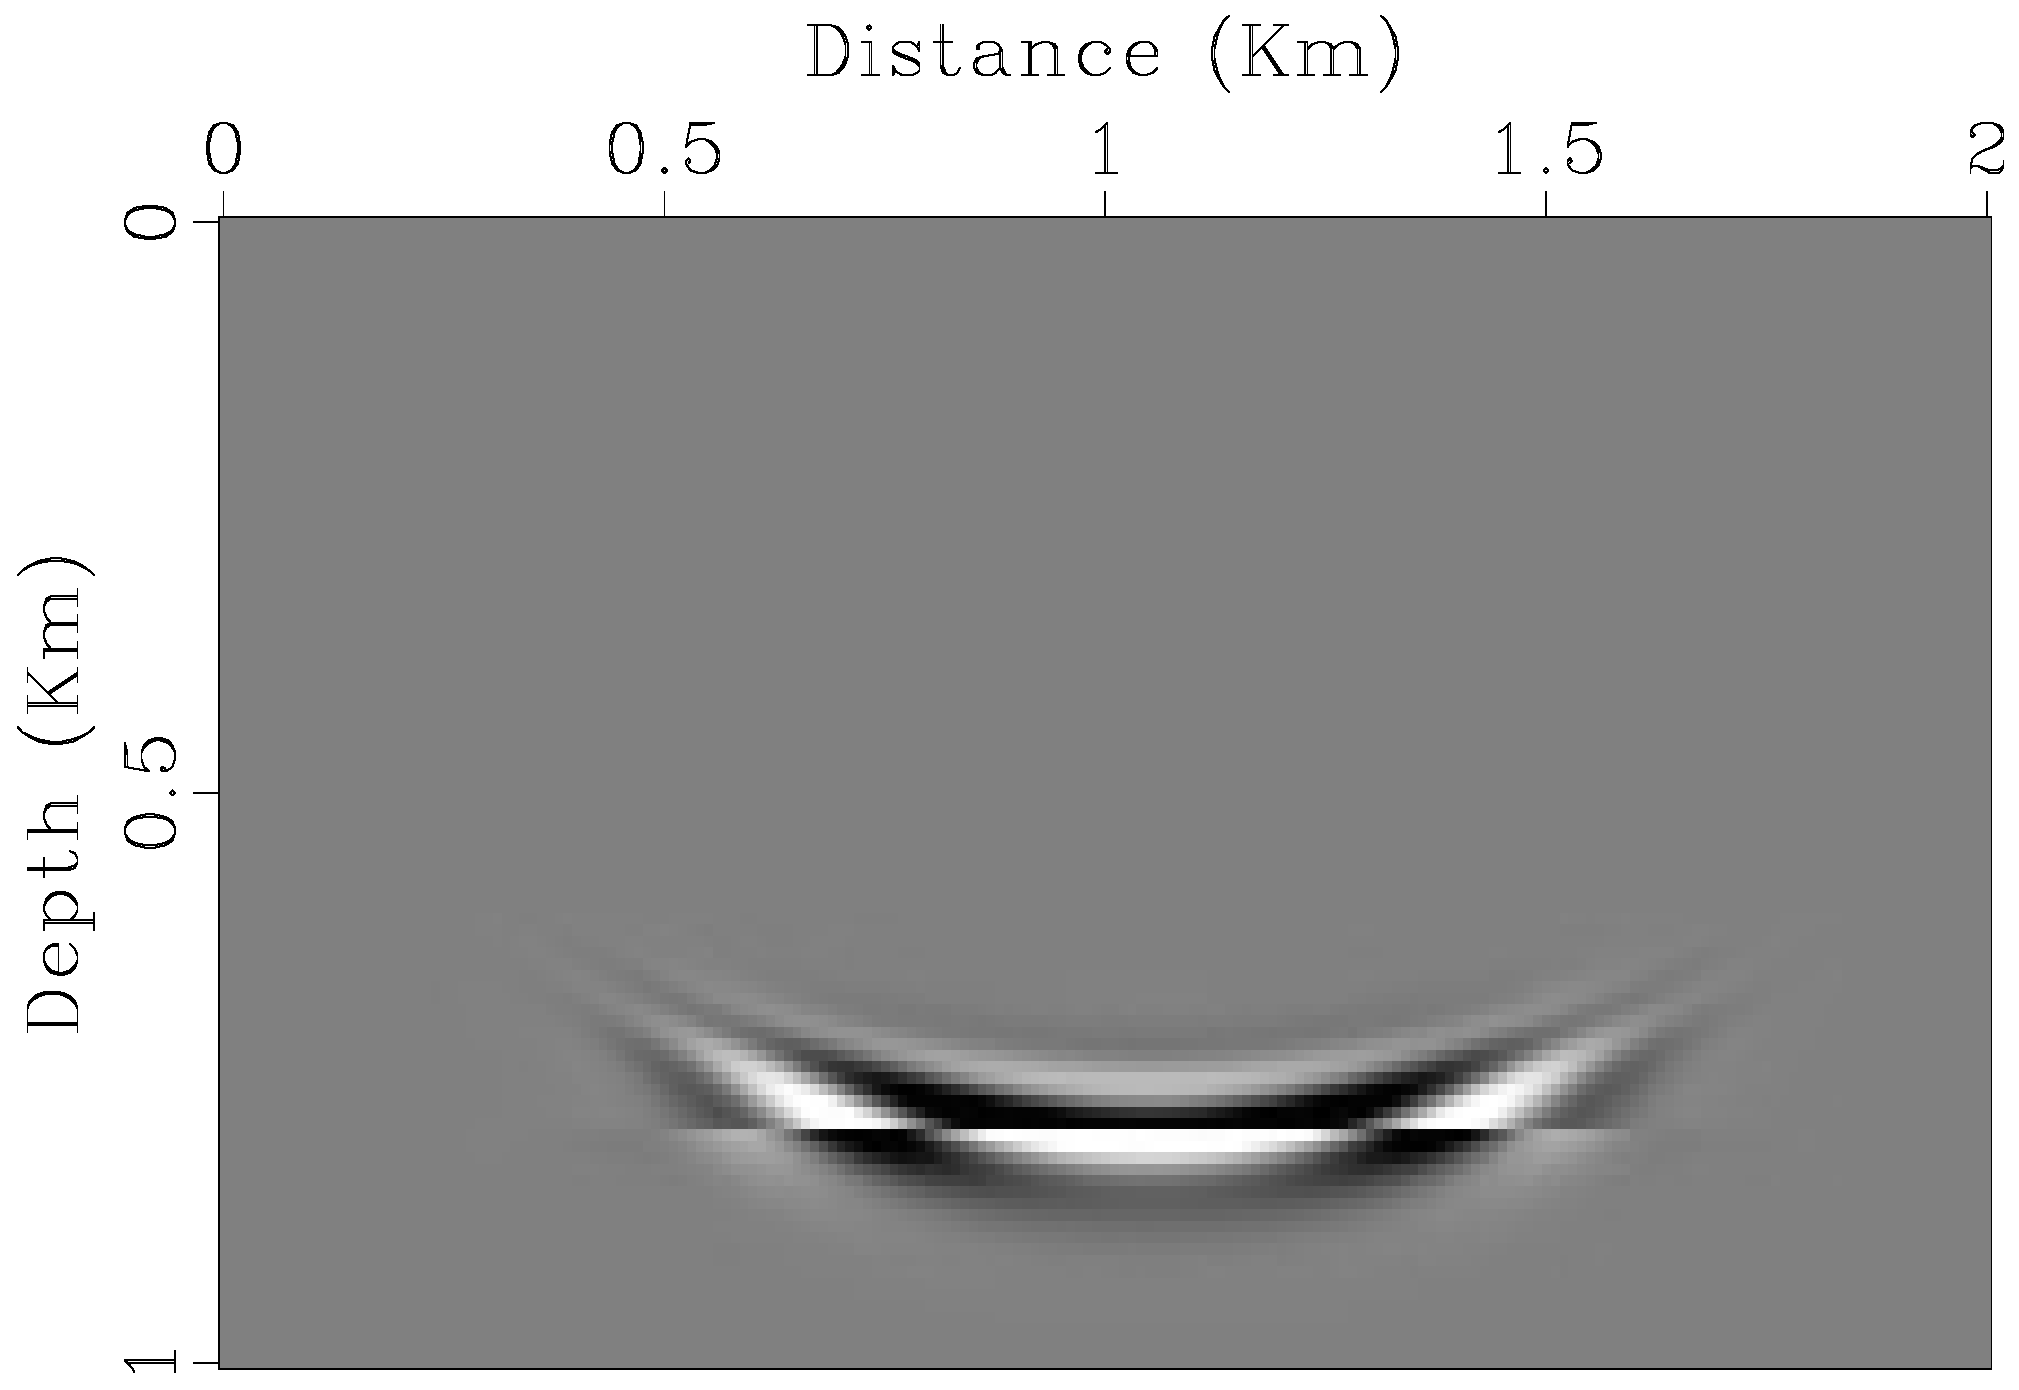
\includegraphics[width=0.45\linewidth]{figure/grad3}}
    \fcaption{两层介质$Q$-RWI中背景$Q$的子梯度。(a)源端梯度;(b)检波点端梯度;
	(c)高波数奇异分量。}{Sub-gradients of $Q$-RWI for simple two-layer model: 
	(a) sourece-side reflection gradient; (b) receiver-side reflection gradient; 
	and singular component.}[两层介质$Q$-RWI中背景$Q$的子梯度]
    \label{fig:grad_qrwi}
\end{figure*}

$Q$-RWI的梯度公式(\ref{eq:gradient})共包含三项。如图~\ref{fig:grad_qrwi}所示,
第一二项”兔耳朵“状的梯度,提供了沿反射波路径的低波数的背景$Q$的更新量。第三项对应于
反射波在成像点的成像结果,对RWI来说是奇异的非光滑的分量。第三项会在反射界面位置更新
高波数成分从而增加反演的非线性程度。在声波的RWI中,\citeB{wu.alkhalifah:2015}观察到
第三项在反射界面处的值的符号与第一二项在反射界面处的值相反,但是数值不一样。他们将
将第三项加入反演中,通过求解一个内部优化问题,用第三项来减弱第一二项在反射界面处
的影响以降低反演的非线性程度。为了不增加反演的计算量,在$Q$-RWI中我们省略掉第三项,
同时用Poynting矢量来简单区分上下行波(\citeA{yoon.marfurt:2006}),
以减弱梯度在反射界面处的奇异性。由图~\ref{fig:grad_poynting}可以看出,无论是单炮单道、
单炮多道还是多炮多道叠加,用Poynting矢量来进行上下行波分离的预条件都减弱了$Q$-RWI中
梯度在反射界面处的奇异性,从而增强了反演的稳定性。以上的$Q$-RWI梯度是基于SLS粘声方程
推导的,这套推导方法同样适合于常$Q$粘声方程,其具体推导可参见附录B。

\begin{figure*}[!htbp]
    \centering
    \subfigure[]{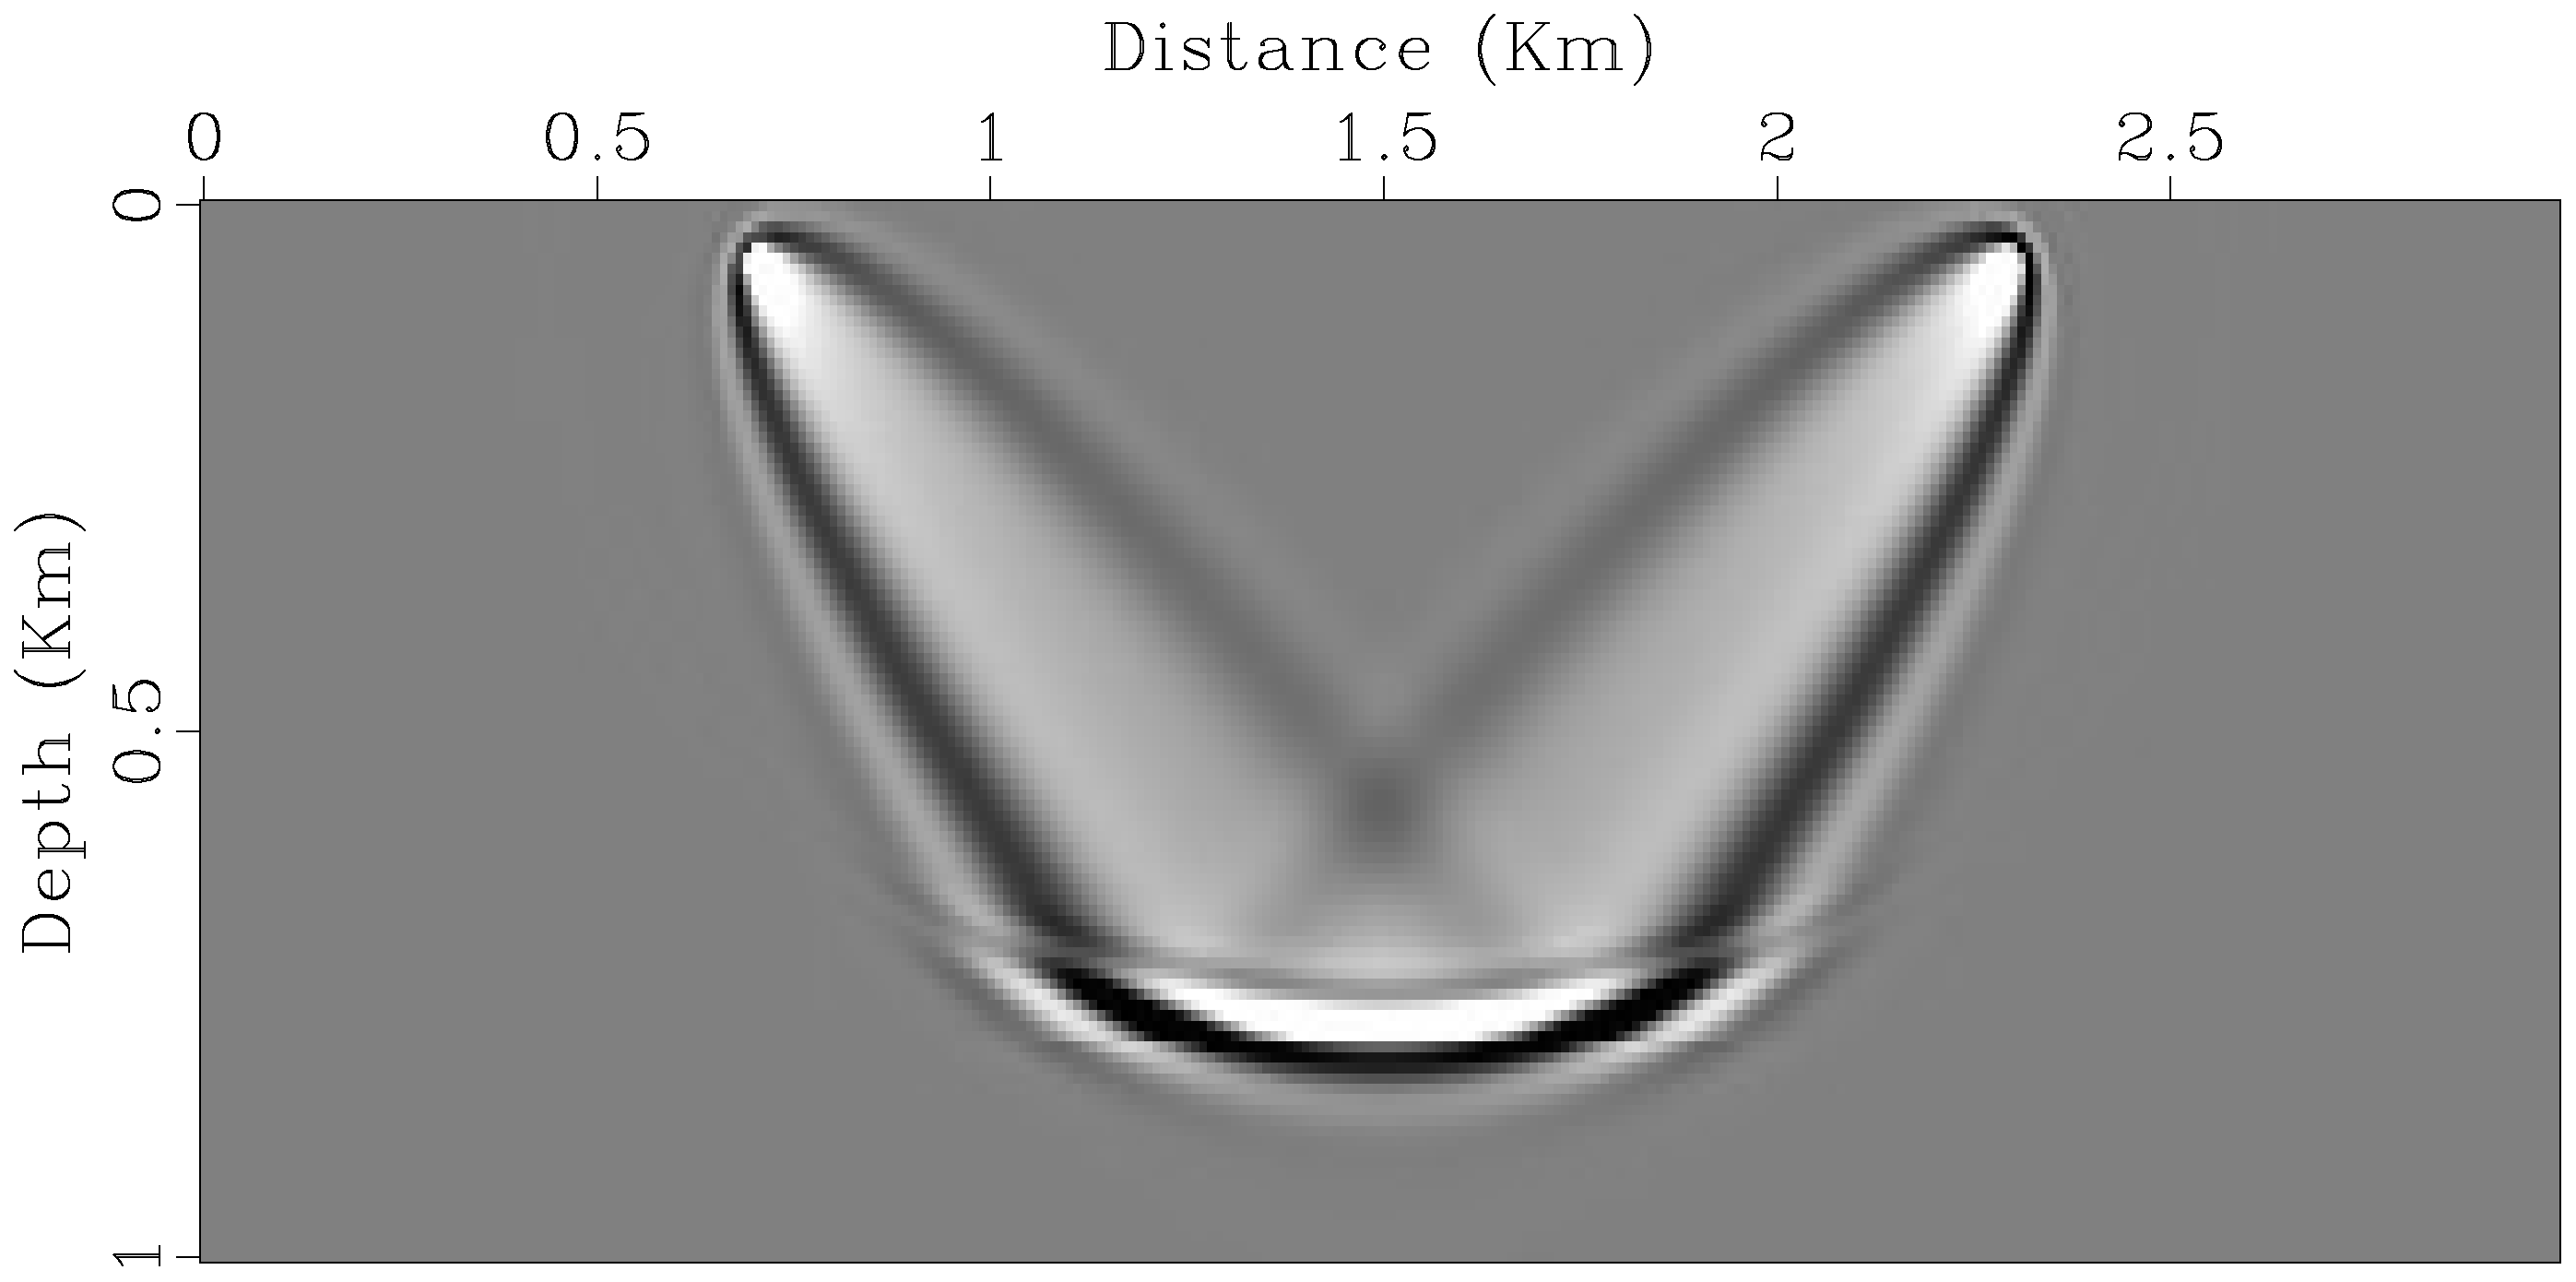
\includegraphics[width=0.45\linewidth]{figure/grad_rwi}}
    \subfigure[]{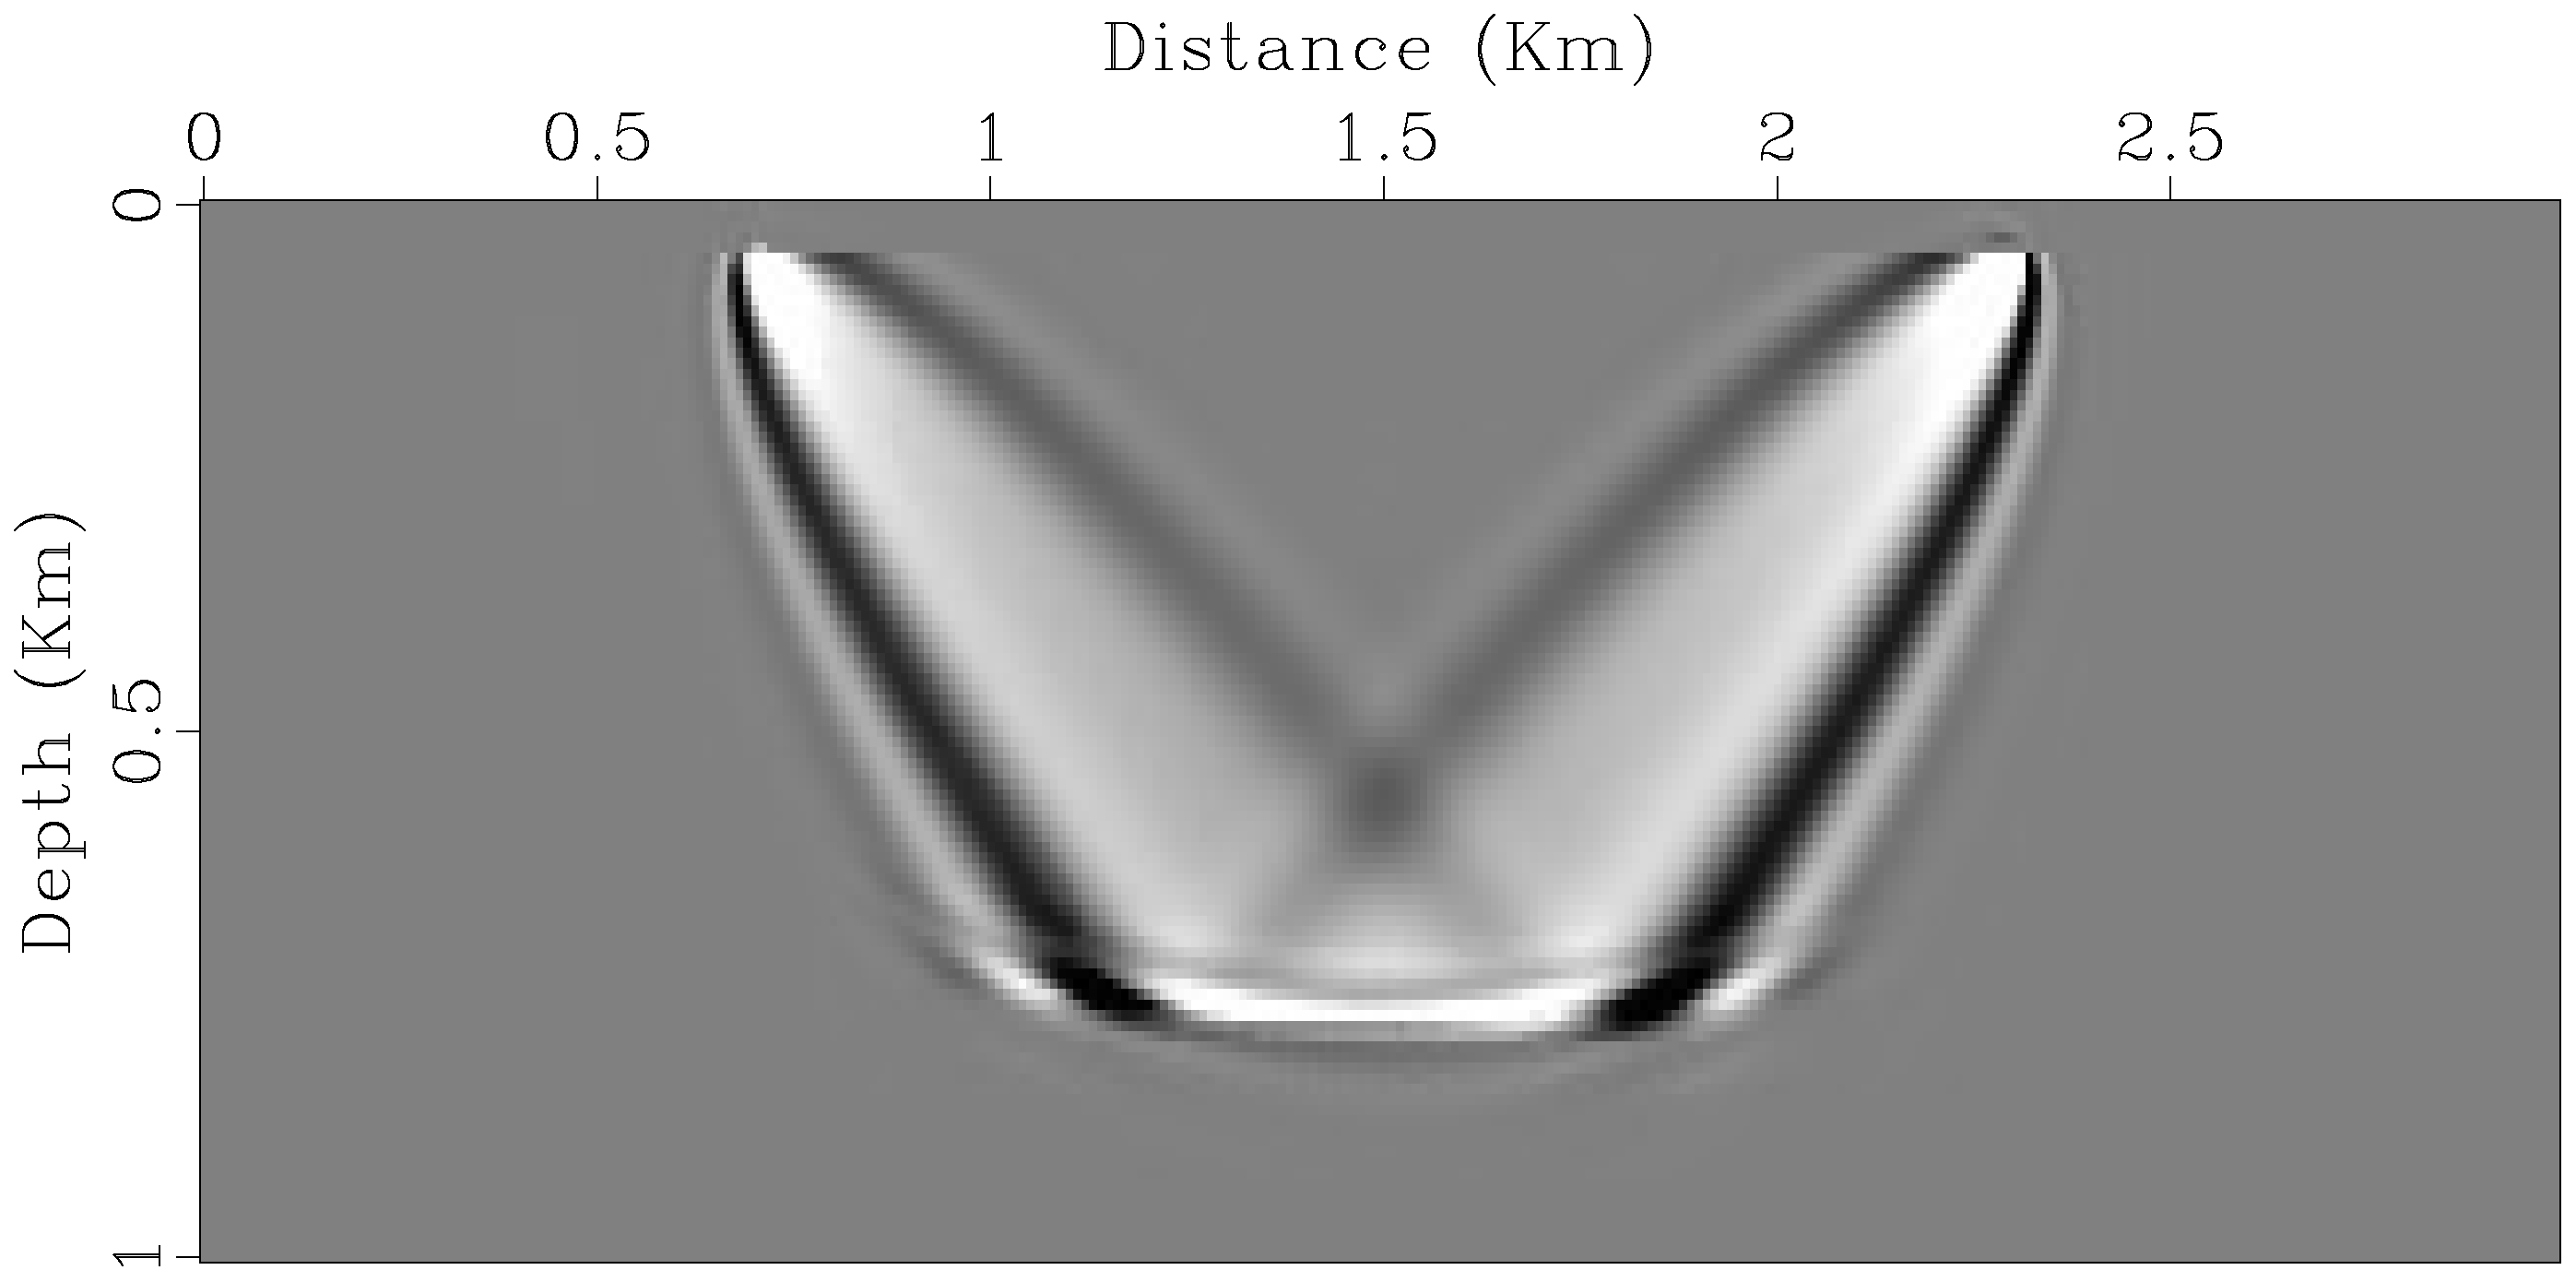
\includegraphics[width=0.45\linewidth]{figure/grad_rwi_poynting}}
    \subfigure[]{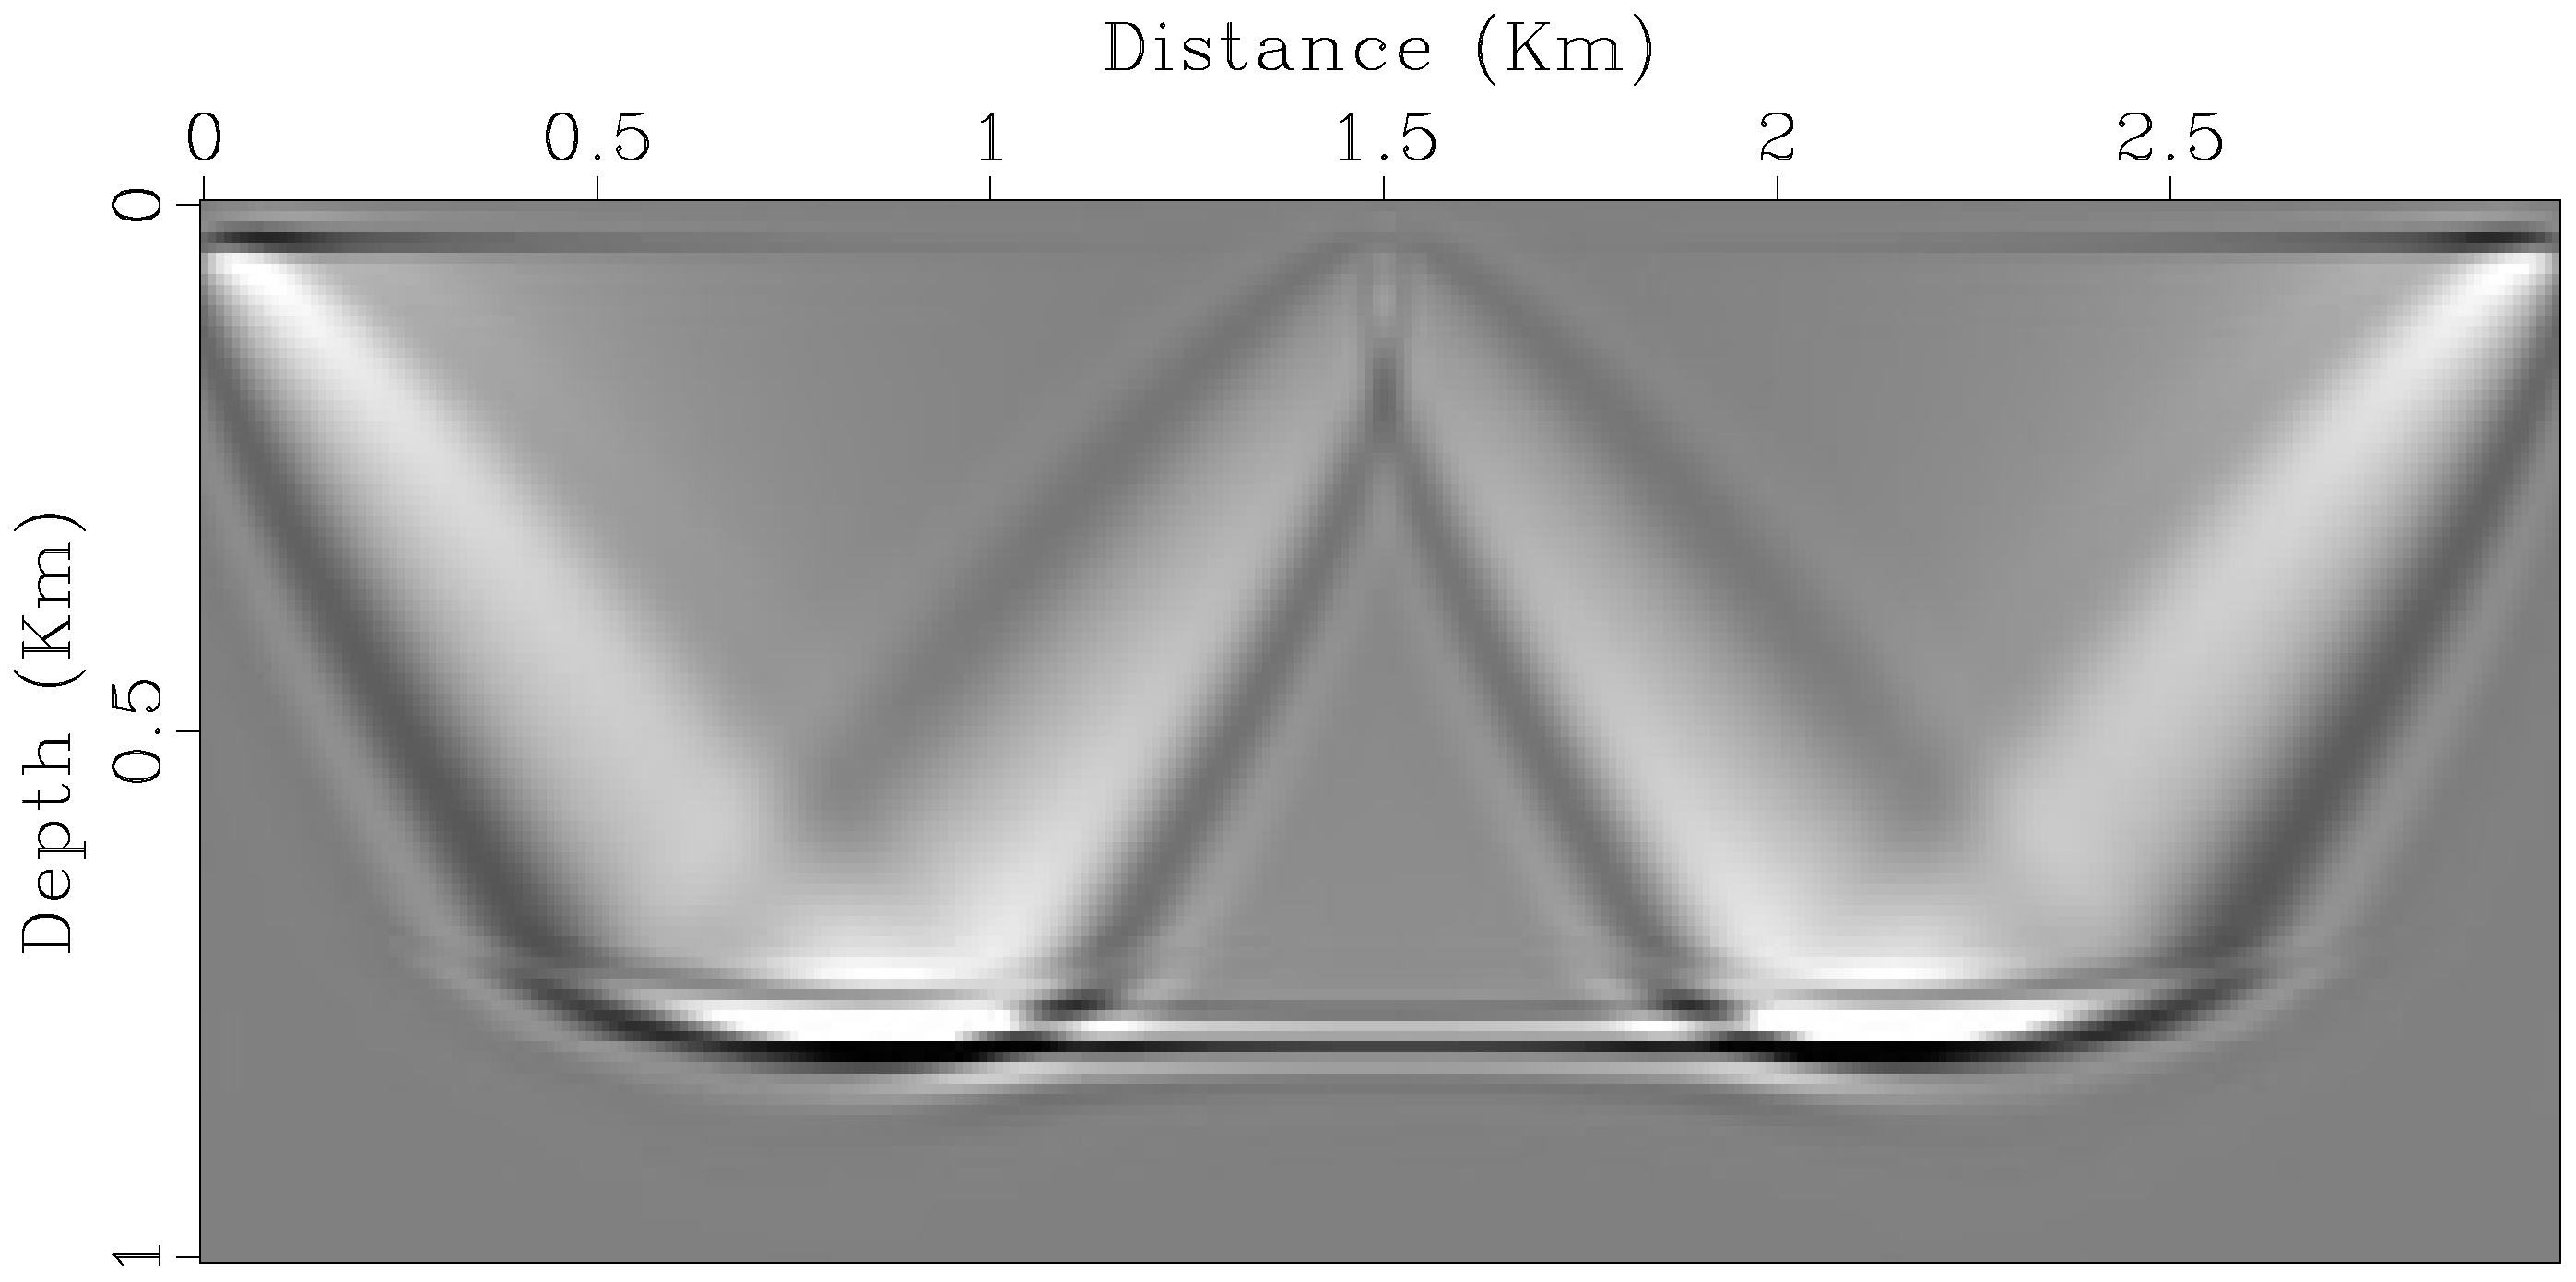
\includegraphics[width=0.45\linewidth]{figure/grad_rwi_oneshot}}
    \subfigure[]{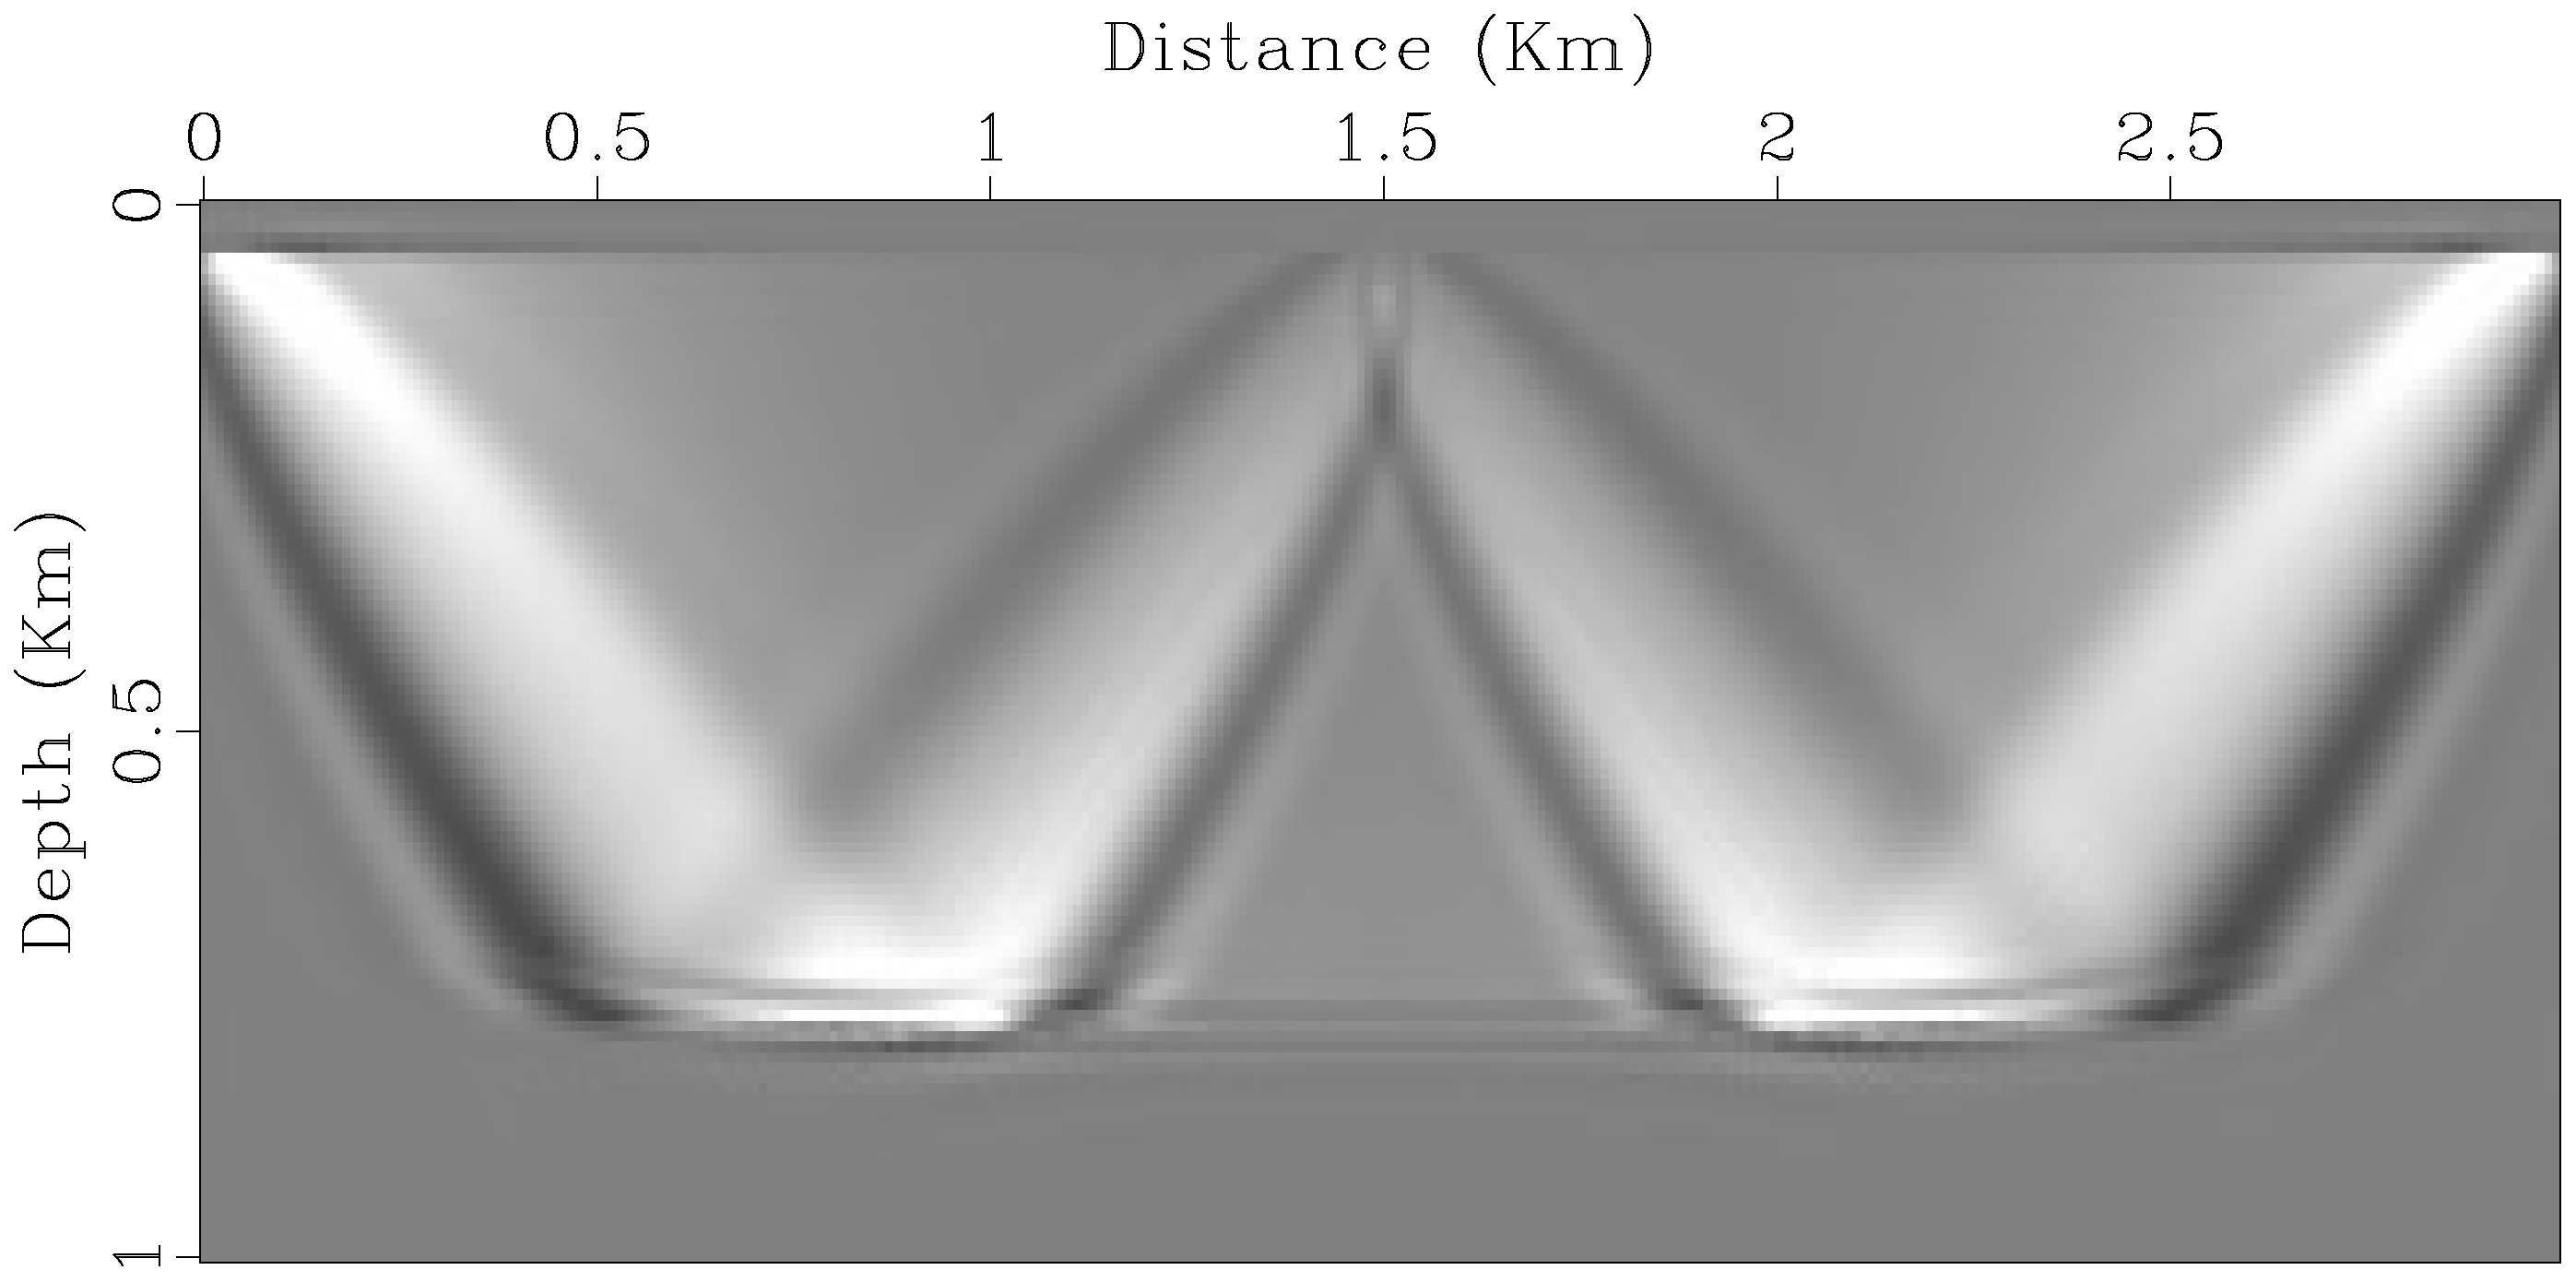
\includegraphics[width=0.45\linewidth]{figure/grad_rwi_poynting_oneshot}}
    \subfigure[]{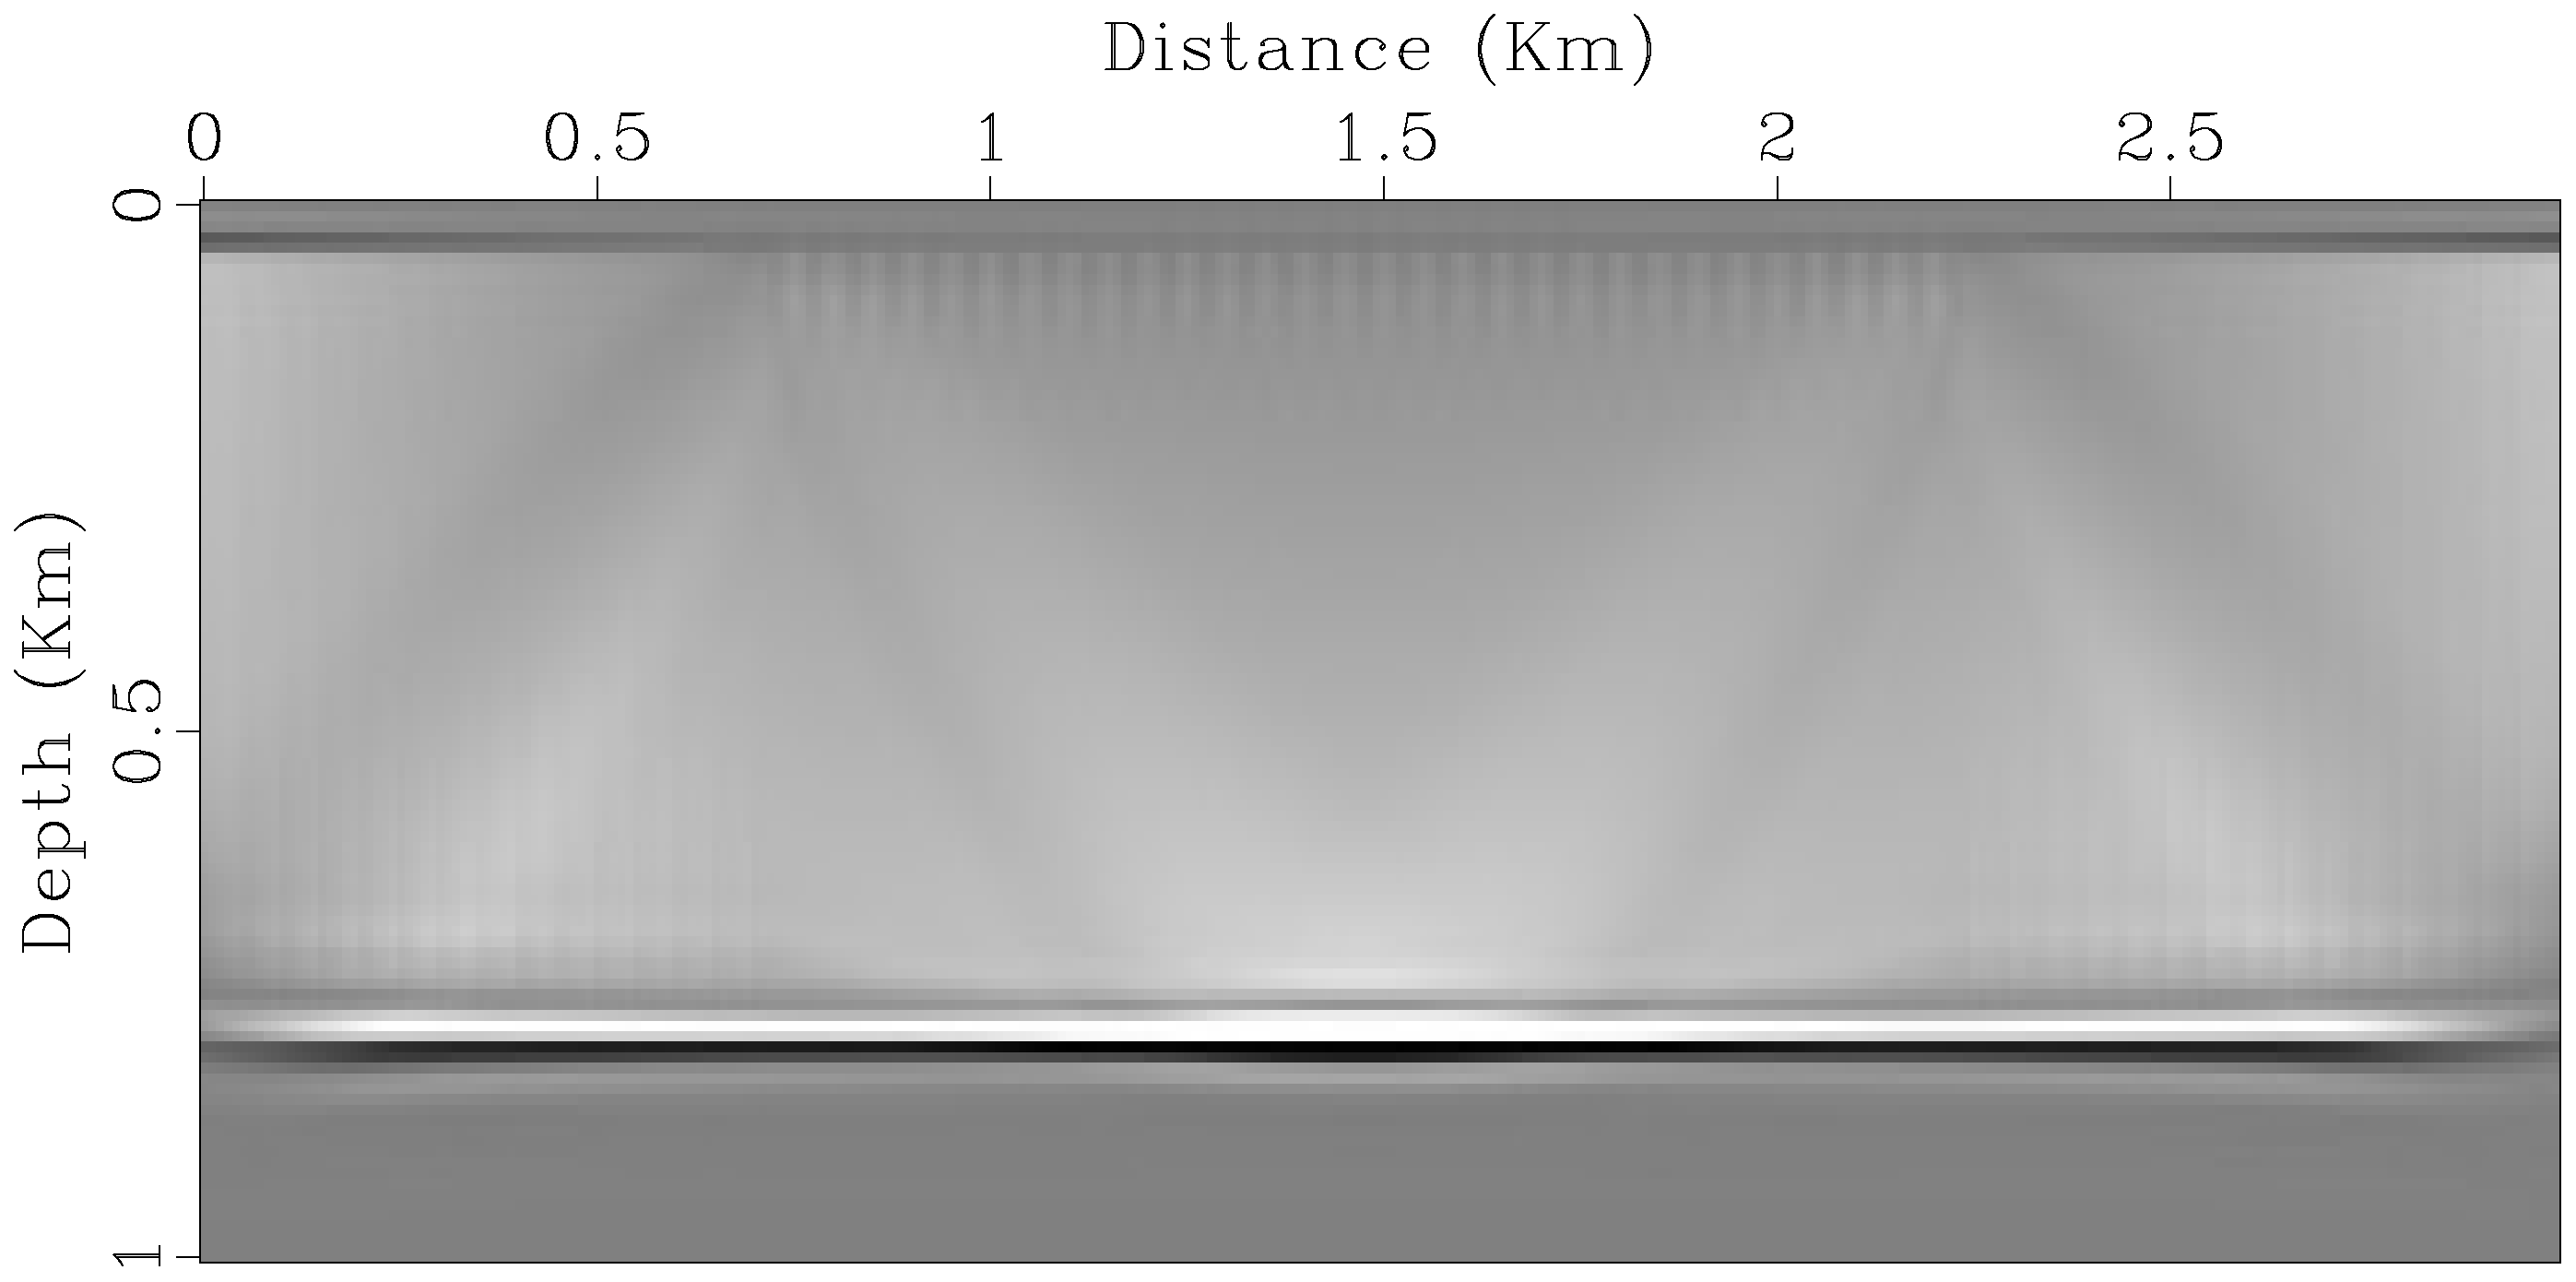
\includegraphics[width=0.45\linewidth]{figure/grad}}
    \subfigure[]{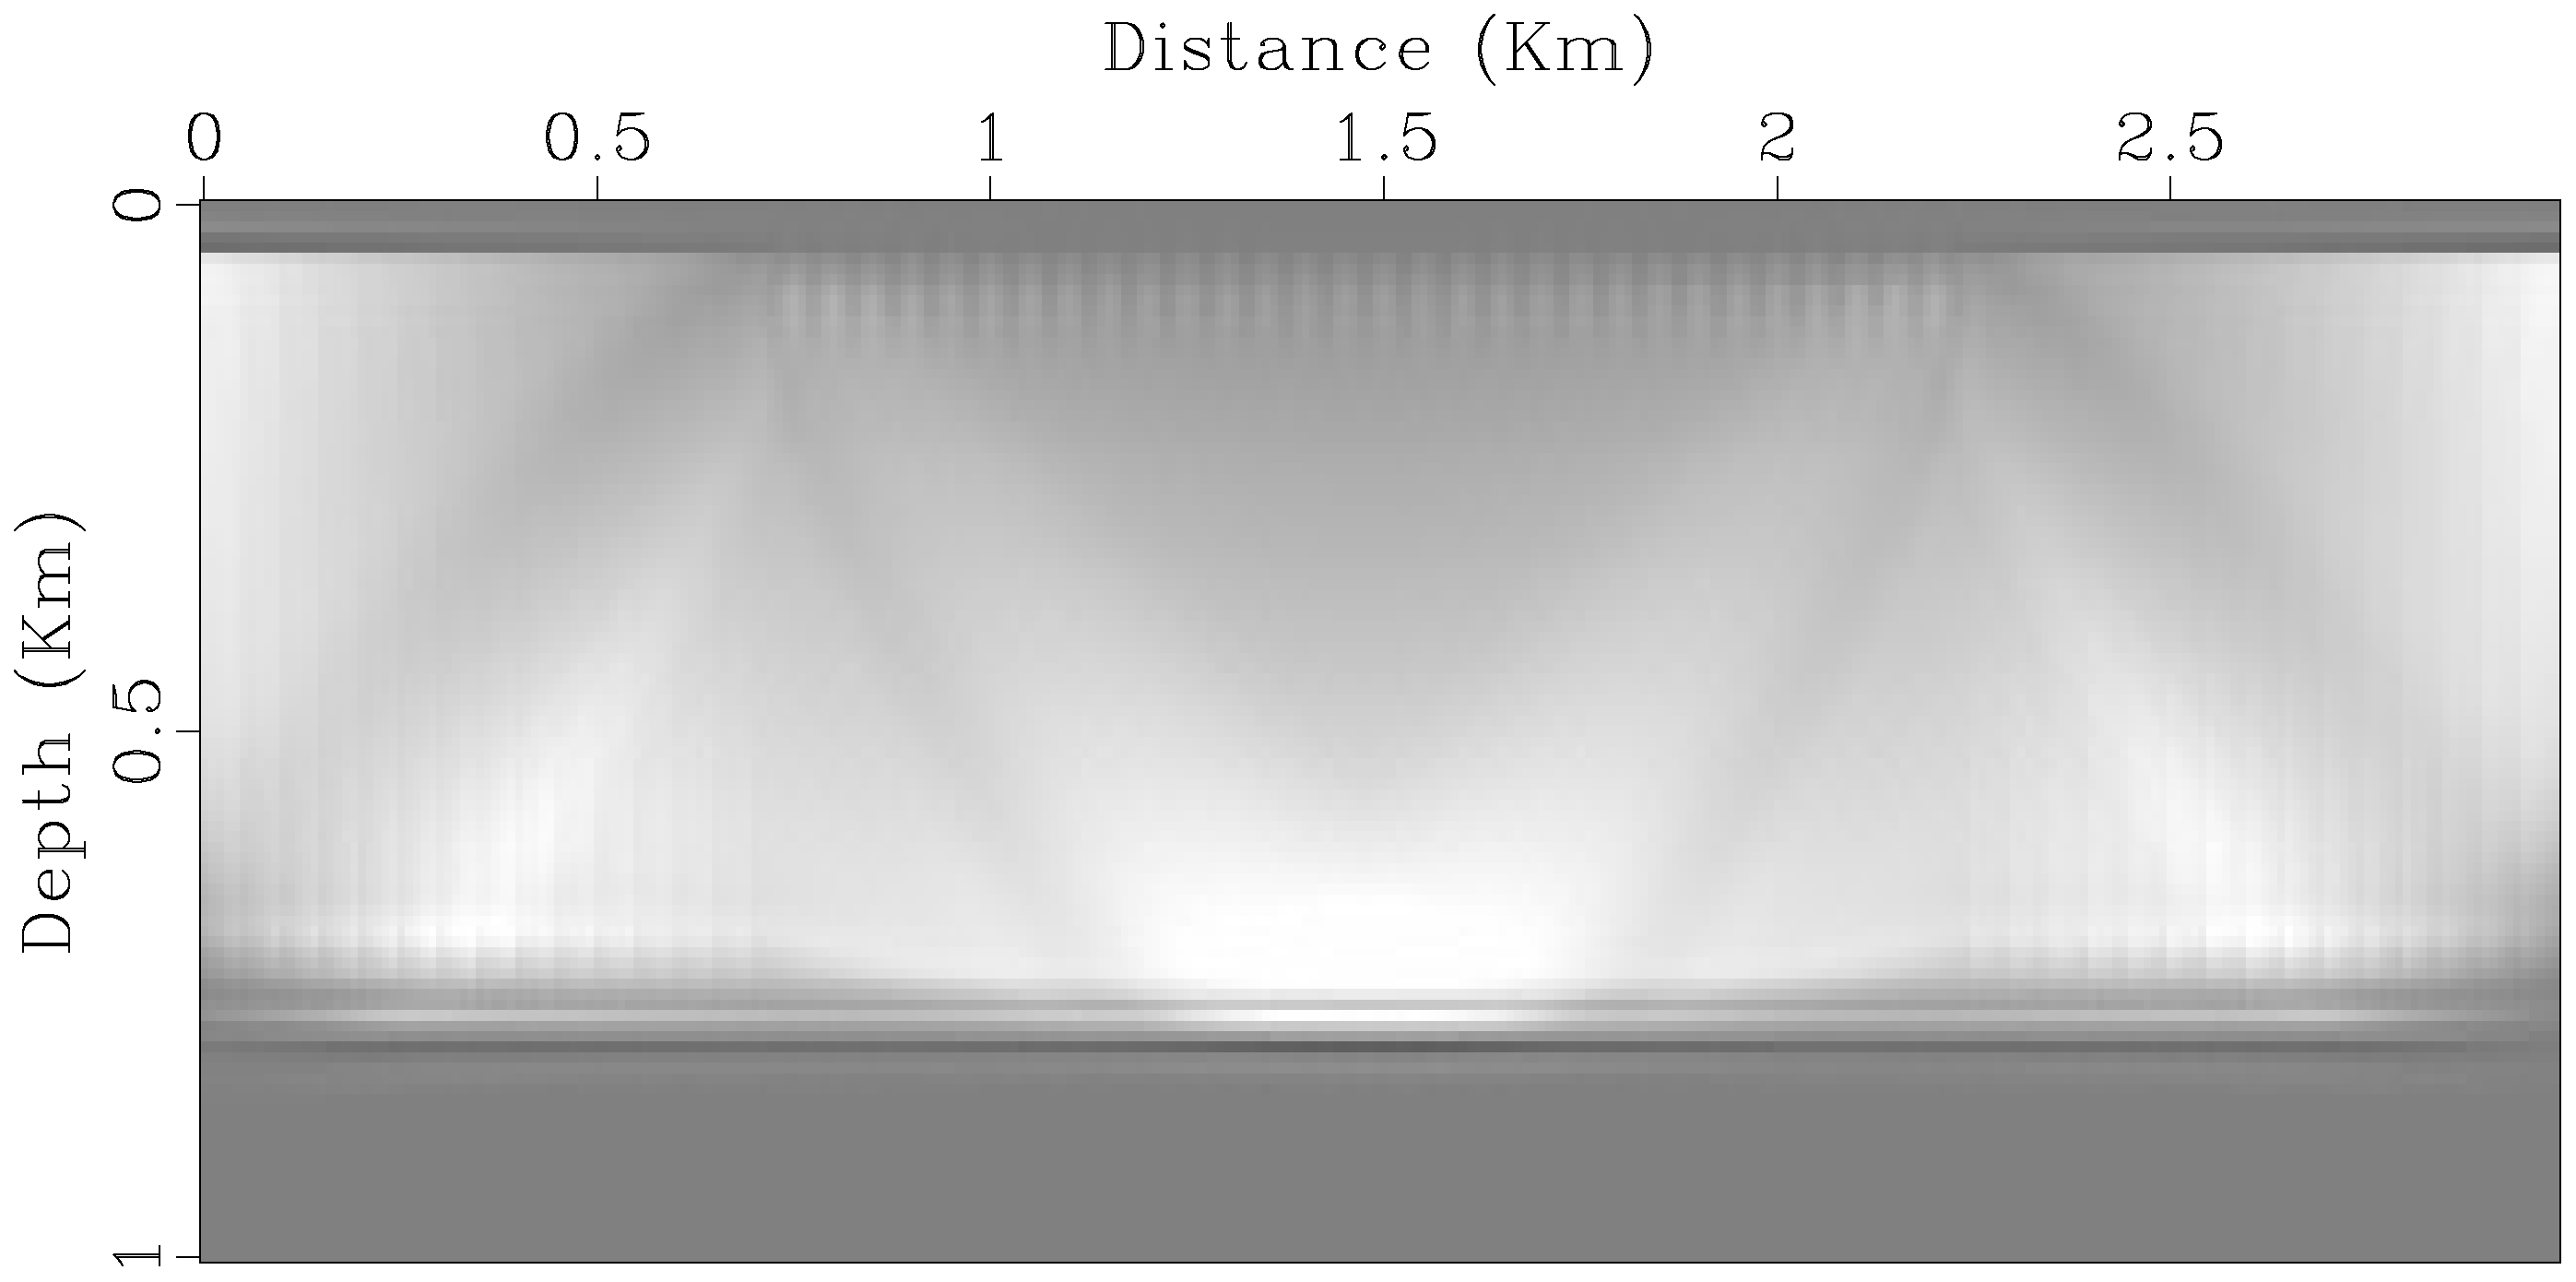
\includegraphics[width=0.45\linewidth]{figure/grad_poynting}}
    \fcaption{两层介质Poynting矢量预条件梯度对比,左边是没有预条件的梯度,右边是通过
	Poynting矢量上下行波分离预条件的梯度。(a,b)单炮单道;(c,d)单炮多道;
	(e,f)多炮多道。}{Comparison the gradients before and after using Poynting vector 
	for preconditing for simple two-layer model, the left column are before precondition 
	gradients and the righ column are after precondition results. (a, b) one shot and one 
	trance; (c, d) one shot and multi-trances; (e, f) multi-shots and multi-trances. 
	}[两层介质Poynting矢量预条件梯度对比]
    \label{fig:grad_poynting}
\end{figure*}

计算出梯度之后,$\tau(\mathbf{x})$可用最速下降法来迭代求解:
\begin{equation}
    \tau(\mathbf{x})^{(k+1)}=\tau(\mathbf{x})^k-\alpha \mathbf{P_c}(\mathbf{x})
    \frac{\partial \mathcal{L}}{\partial \tau(\mathbf{x})},
\end{equation}
式中$k$是迭代次数,$\mathbf{P}_c(\mathbf{x})$是预条件算子,步长$\alpha$可通过
任何反向追踪的线性搜索方法求解(\citeA{nocedal:1999})。在每一个迭代步内,
当$\tau(\mathbf{x})$更新之后可用方程~\ref{eq:tq}将其转换为$Q(\mathbf{x})$。


\newpage
\section{数值实验}
本节用一个层状模型(图~\ref{fig:lens_model})来验证$Q$-RWI的有效性。该模型
宽4km,深2.5km。在模型的表面均匀分布20炮,炮间距为200m,检波器对称分布于震源
的两端,间距为10m且最大偏移距为1km。用峰值频率为30Hz的雷克子波作为爆炸震源。
在模型的中深部包含一个强的$Q$异常体,最小$Q$值达到30。在反演的过程中认为体积
模量$K_0$和$\delta K$都是已知的,并且密度为常数。用均匀模型($Q=200$)作为
初始模型。

如图~\ref{fig:lens_model}c~所示,经过30次迭代之后,$Q$-RWI基本恢复了中深部
的$Q$异常。图~\ref{fig:chouxian}分别抽取了$x=1$km、2km、3km处的伪井曲线。
抽线的结果进一步证明了$Q$-RWI对中深部异常$Q$的恢复能力。由于反射数据在浅层
覆盖不够即波路径在近地表处变窄,使得$Q$-RWI在浅层只能得到一个光滑的等效解。
这也证实了地球物理反问题解的多解性,要处理好这种多解性,在反演时必需加入
先验信息的约束或者多种反演方法相结合,例如$Q$-FWI就能很好的反演浅层$Q$模型。
在模型的最底部,由于没有接收到反射数据,反射波路径没有穿过该区域,所以没法
正确反演。图~\ref{fig:misfit_model}展示了迭代过程中的收敛曲线,在这种理想
的合成数据中,目标泛函下降了七八个数量级,这也有力的证实了$Q$-FWI框架的合理
性。图~\ref{fig:record_diff}展示了在$x=2$km 处第10炮观测记录;观测数据与初始
模型模拟数据的残差以及观测记录与30次迭代之后模拟数据的残差。经过30次迭代之后
模拟数据与观测数据之间的残差基本为零,这也更好的证明了$Q$-RWI的有效性。

最后,我们用$Q$补偿的RTM来验证反演结果的可靠性。图~\ref{fig:rtm_model}
分别展示了初始$Q$模型补偿的RTM成像结果、真实$Q$模型补偿的RTM成像结果
以及反演$Q$模型补偿的RTM成像结果。从成像结果中可以看出,初始$Q$模型补偿的RTM
(图~\ref{fig:rtm_model}a)在强衰减区域能量损失严重,并且由于速度频散的影响其成像位
置不对。准确的$Q$模型不仅补偿了强衰减区损失的能量(图~\ref{fig:rtm_model}b),而且也
保持衰减介质中的速度频散关系,从而保证了成像位置的正确性。用$Q$-RWI反演的$Q$模型
补偿的RTM结果(图~\ref{fig:rtm_model}c)与用真实$Q$模型补偿的RTM具有相当的成像
结果。这也从$Q$补偿成像的角度证明了$Q$-RWI反演结果的可靠性。


\begin{figure*}[!htbp]
    \centering
    %{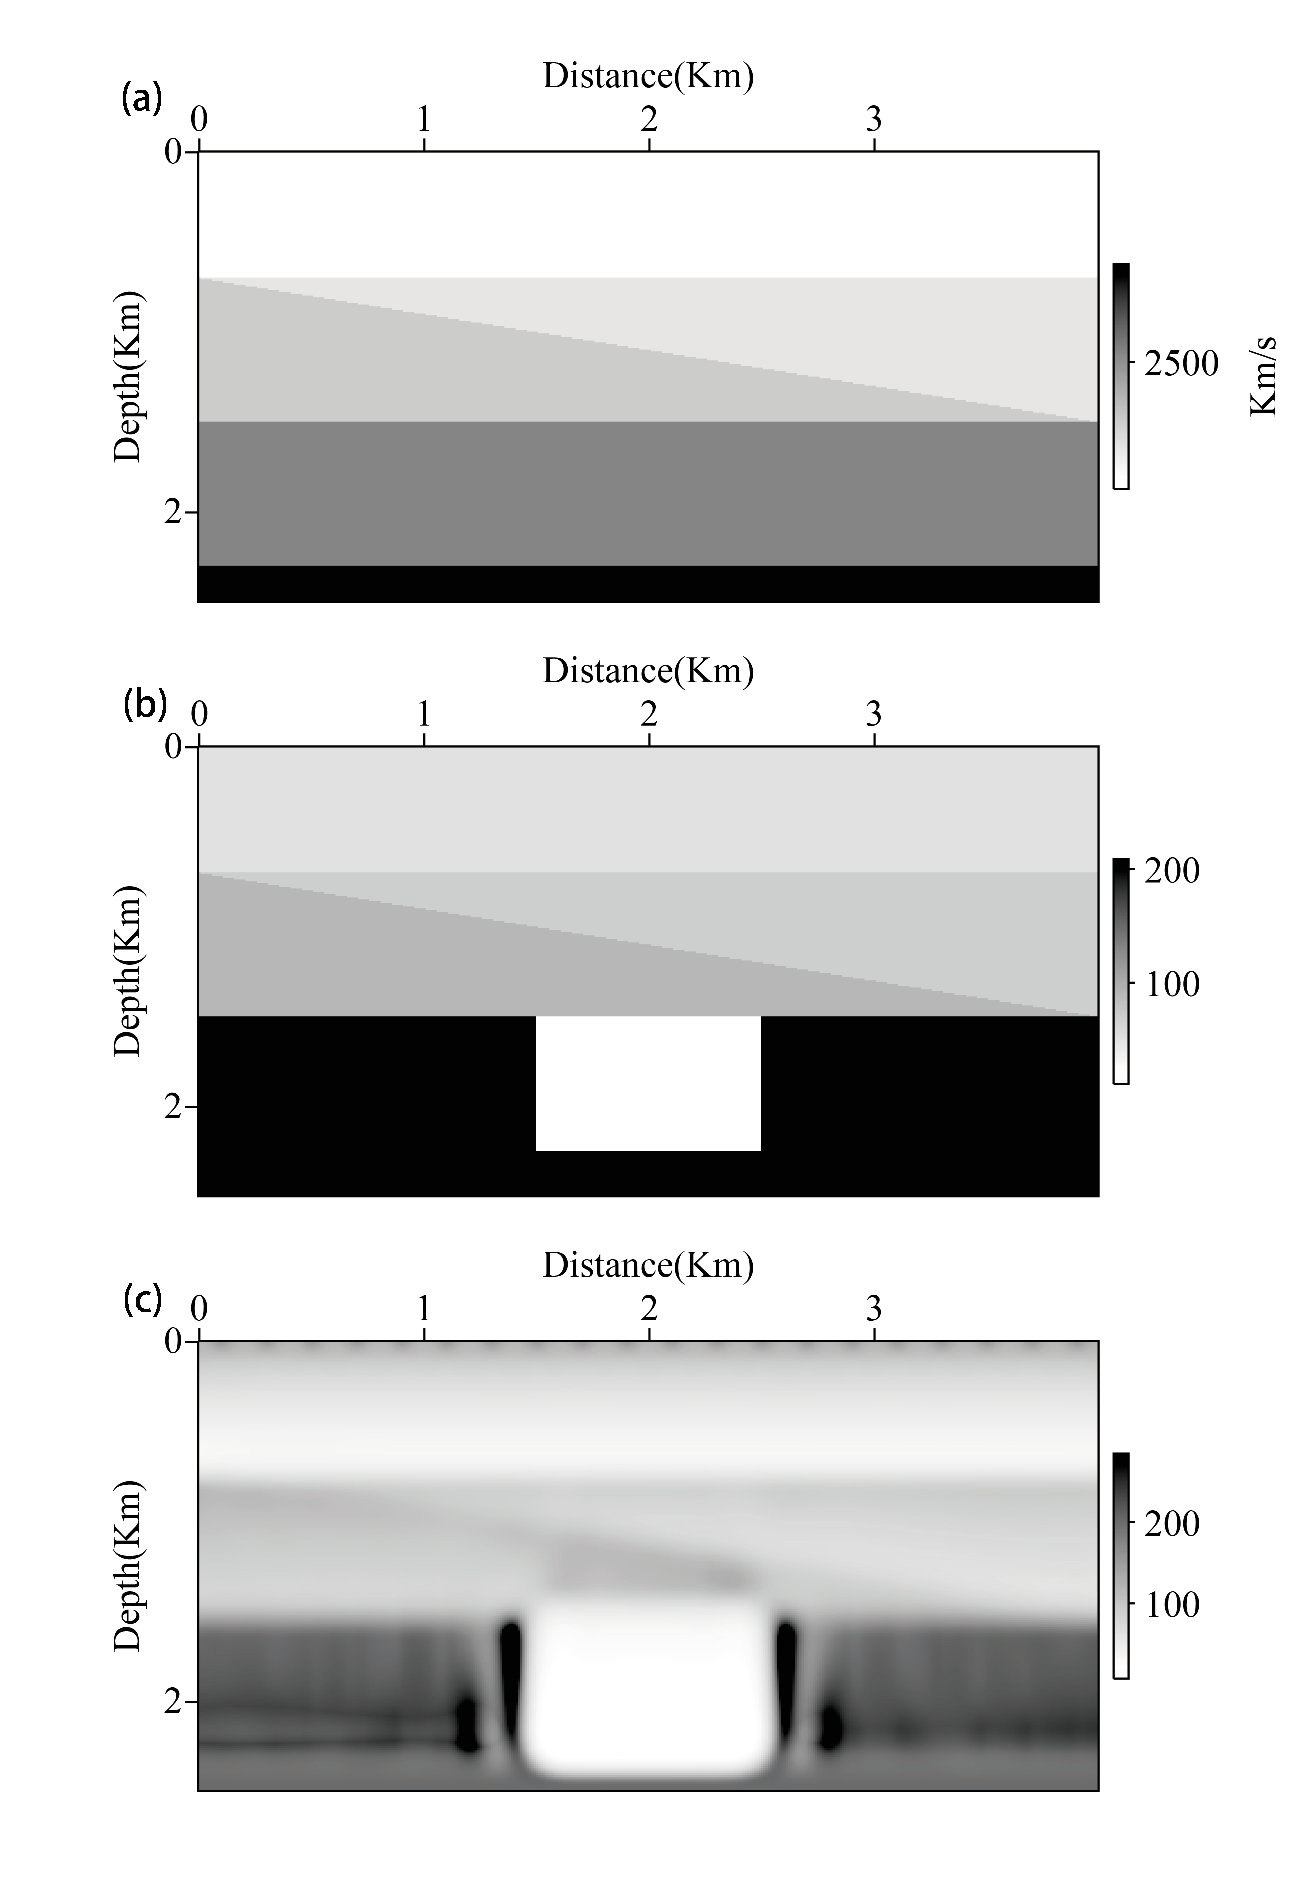
\includegraphics[width=0.85\linewidth]{figure/model}}
	\subfigure[]{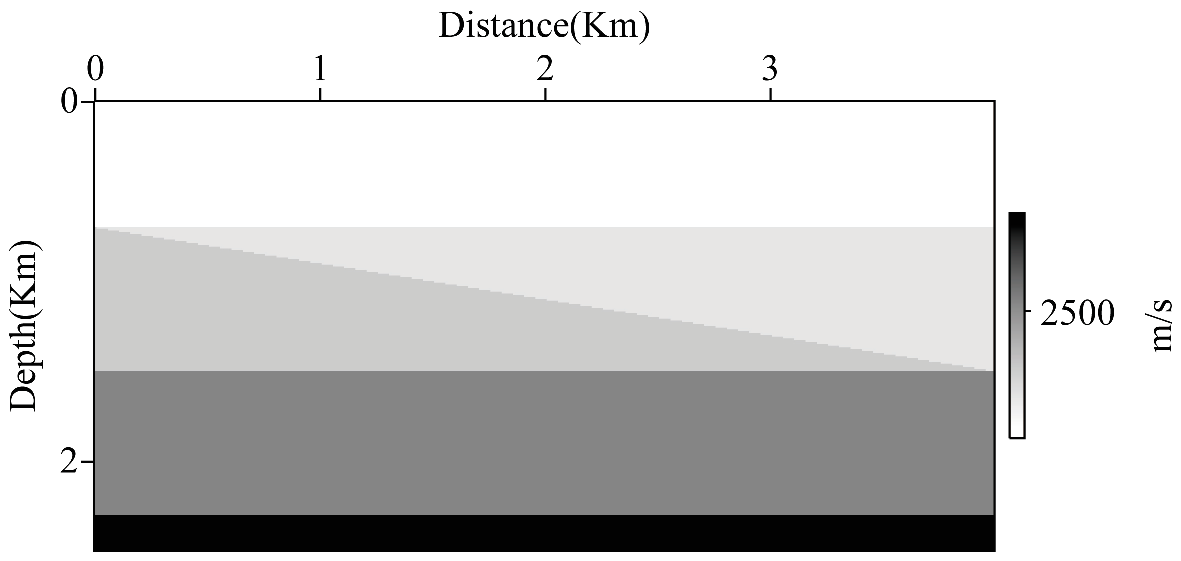
\includegraphics[width=0.82\linewidth]{figure/vel_400x250}}
	\subfigure[]{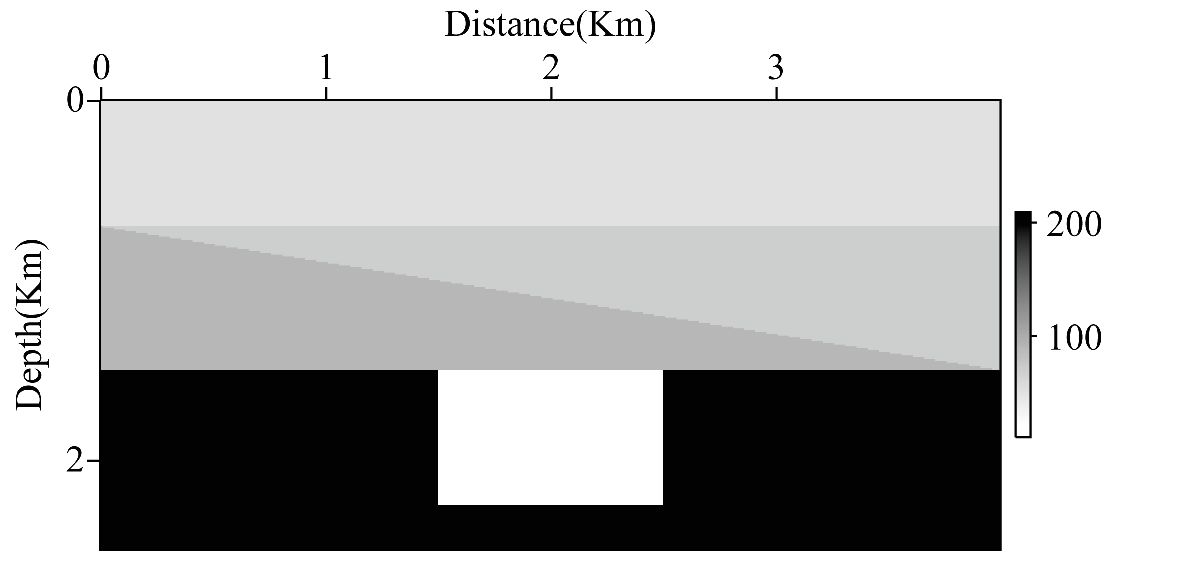
\includegraphics[width=0.82\linewidth]{figure/q_400x250}}
	\subfigure[]{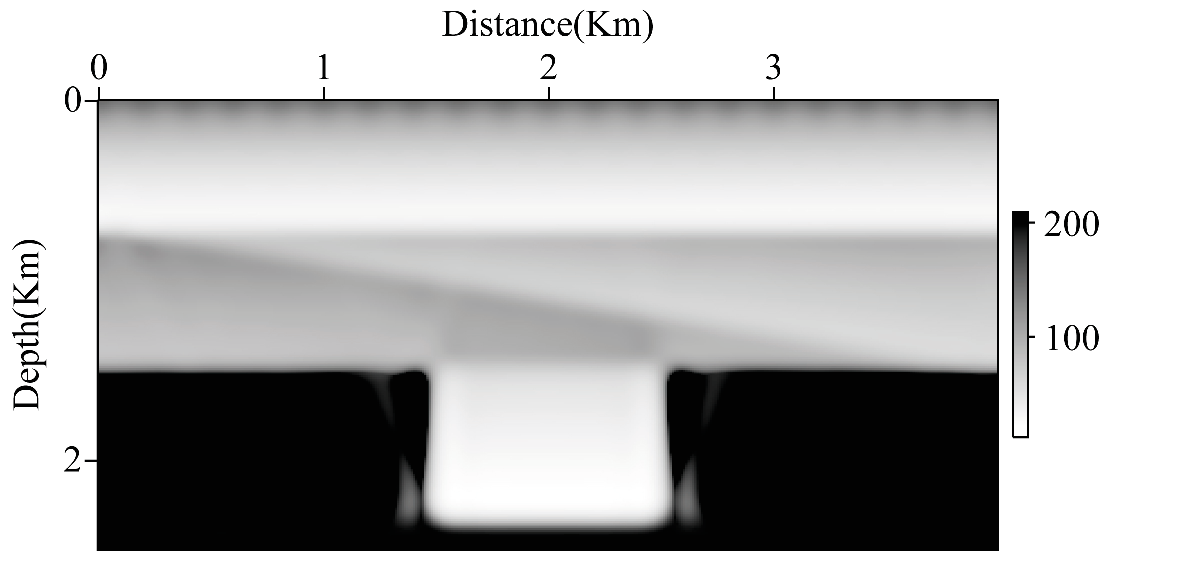
\includegraphics[width=0.82\linewidth]{figure/fq_400x250}}
	\fcaption{层状模型:(a)速度模型;(b)真实$Q$模型;(c)$Q$-RWI
	反演结果。}{The layered model:(a) the velocity model,
	(b) true $Q$ model and (c) inverted $Q$ model using $Q$-RWI.}
	[层状模型]
    \label{fig:lens_model}
\end{figure*}

\begin{figure*}[!htbp]
    \centering
	\subfigure[]{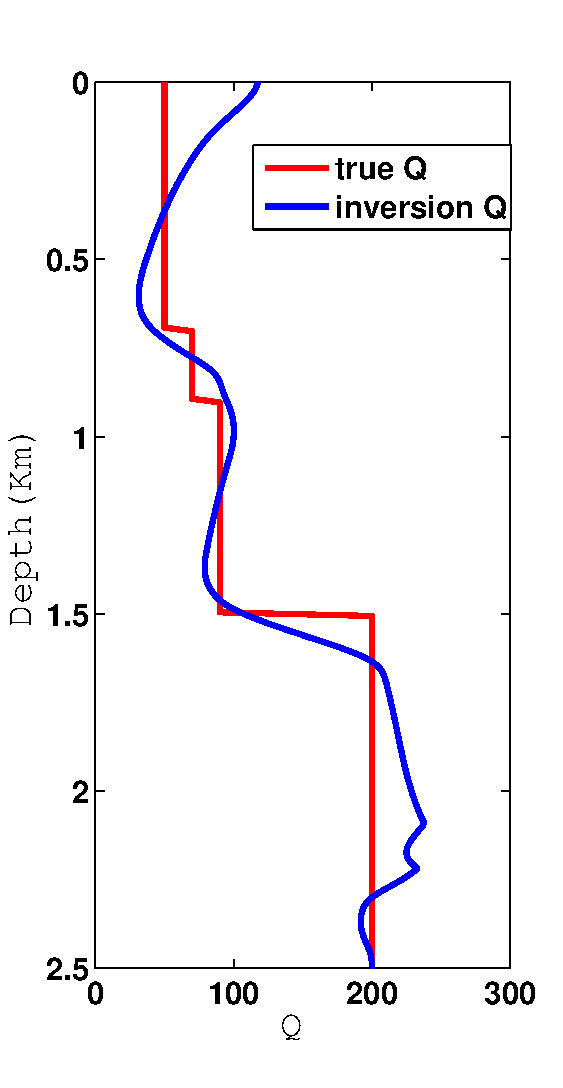
\includegraphics[width=0.32\linewidth]{figure/1km}}
	\subfigure[]{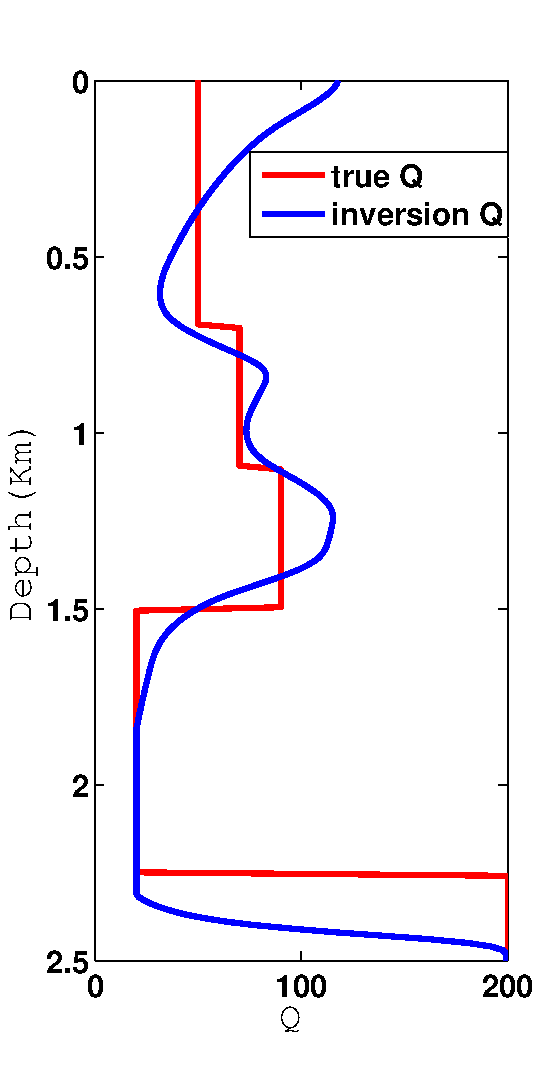
\includegraphics[width=0.32\linewidth]{figure/2km}}
	\subfigure[]{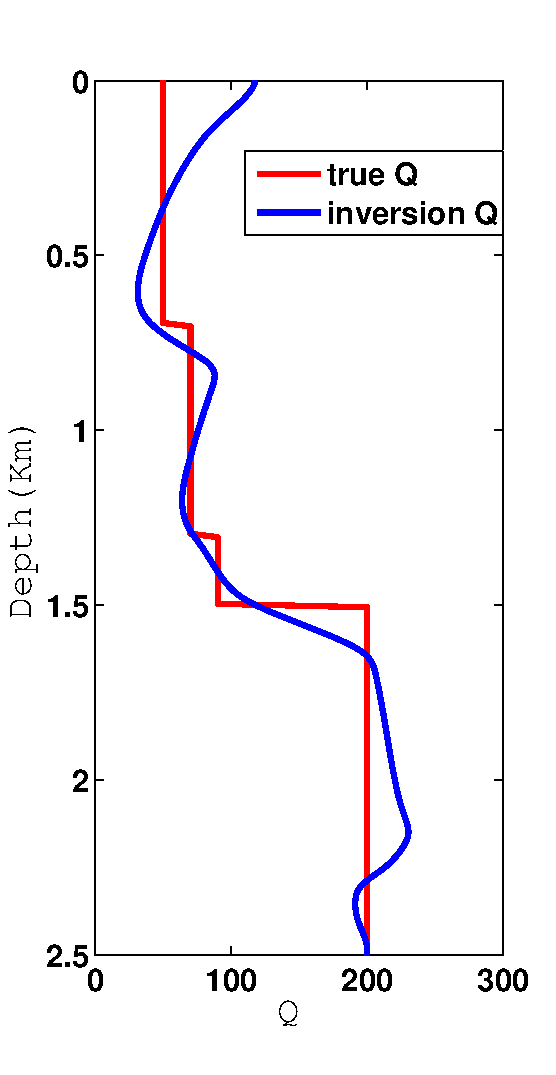
\includegraphics[width=0.32\linewidth]{figure/3km}}
	\fcaption{抽线对比:(a)1km处;(b)2km处;(c)3km处。}{Pseudowells comparison at (a) 1km, (b) 2km
	and (c) 3km.}[抽线对比结果]
    \label{fig:chouxian}
\end{figure*}

\begin{figure*}[!htbp]
    \centering
    {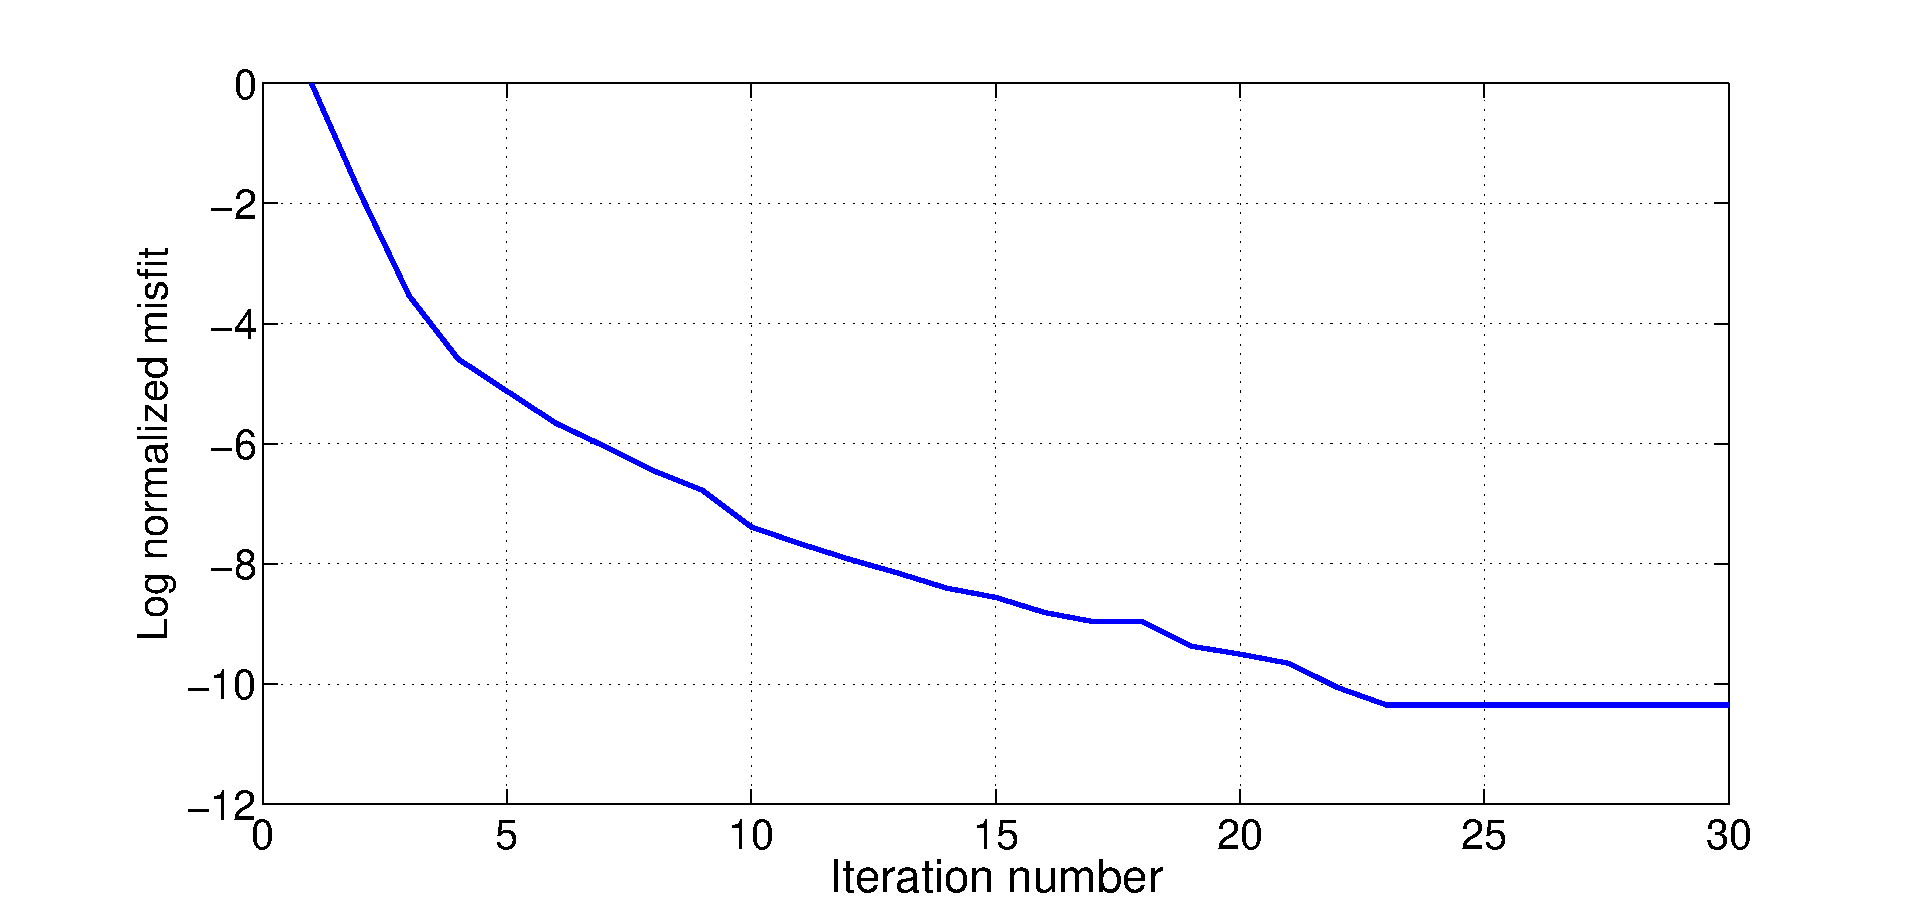
\includegraphics[width=1.0\linewidth]{figure/misfit}}
    \fcaption{收敛曲线}{The history of convergence.}[收敛曲线]
    \label{fig:misfit_model}
\end{figure*}

\begin{figure*}[!htbp]
    \centering
	\subfigure[]{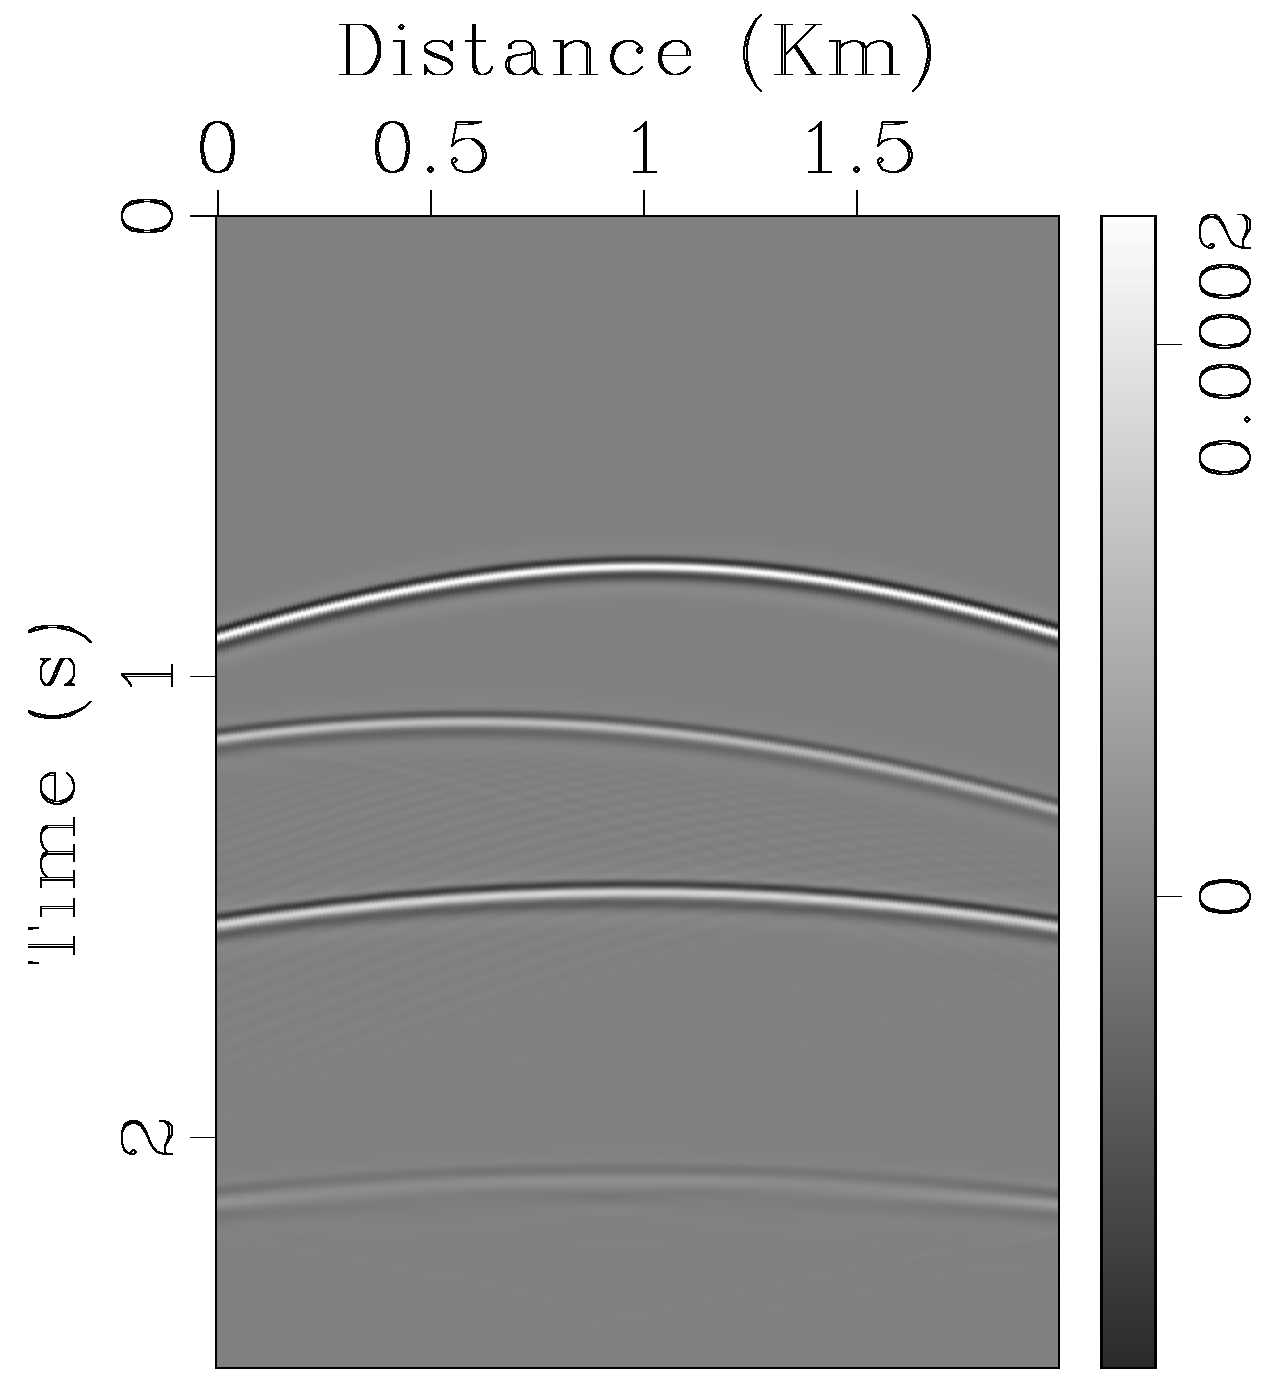
\includegraphics[width=0.47\linewidth]{figure/record}}
	\subfigure[]{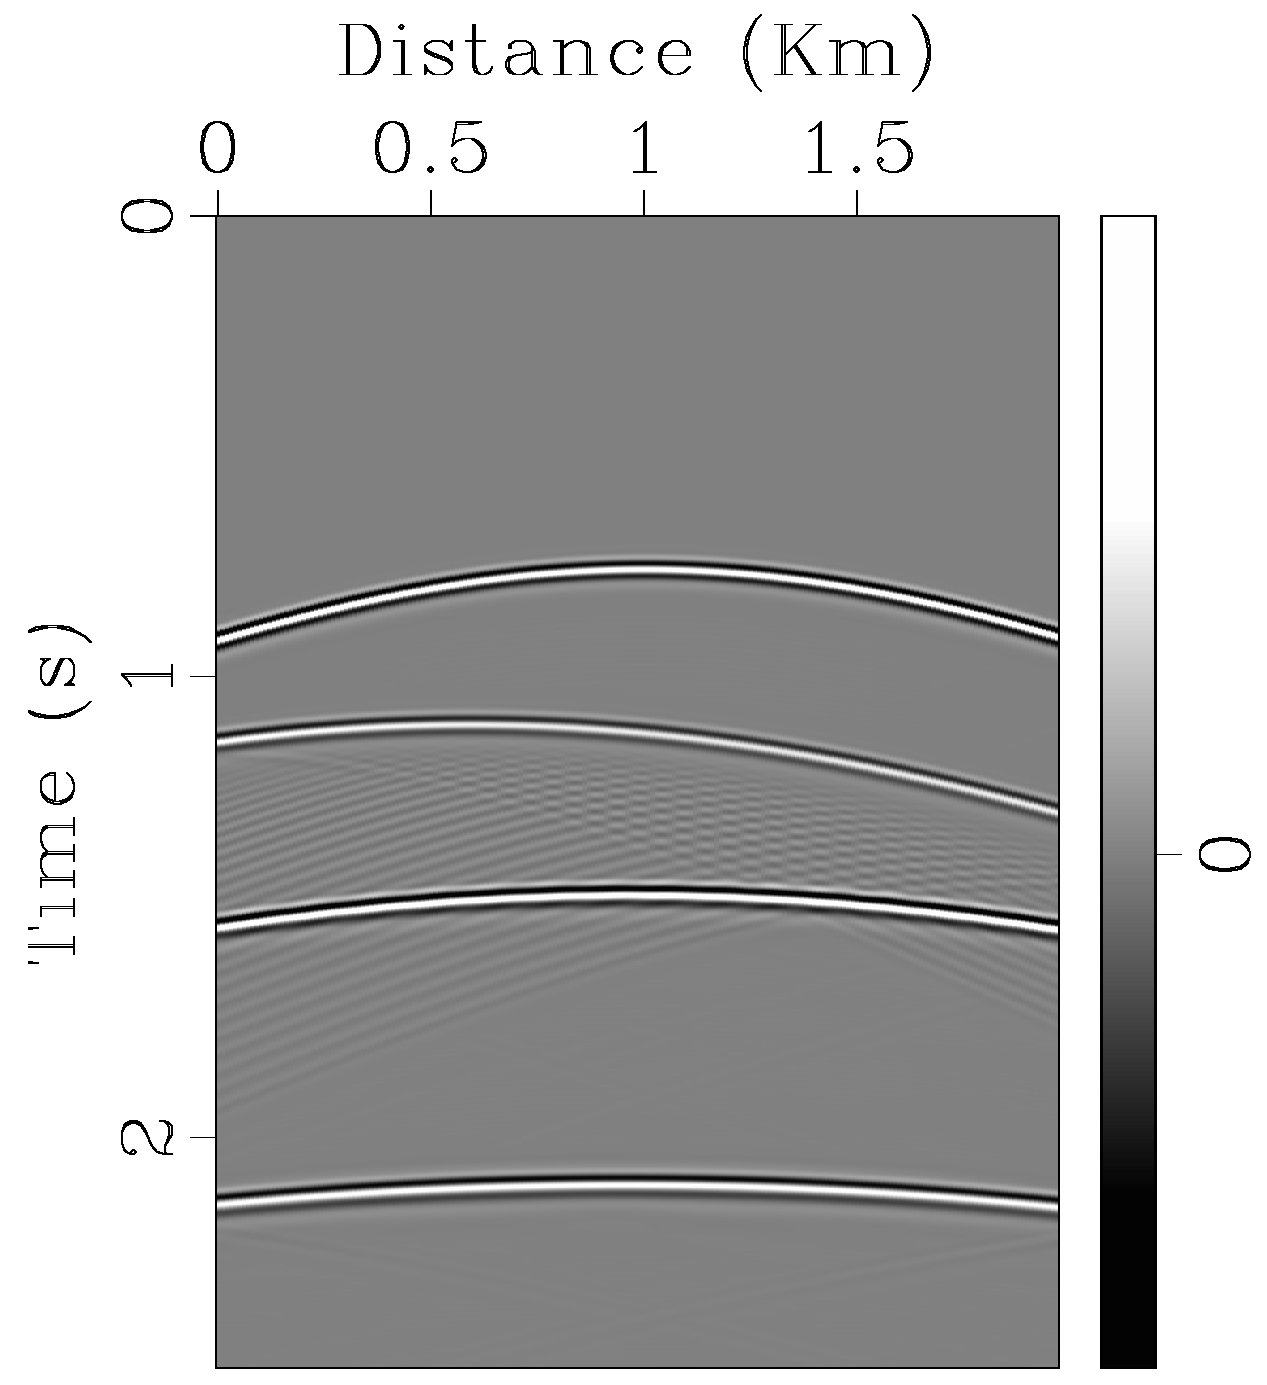
\includegraphics[width=0.47\linewidth]{figure/diff0}}
	\subfigure[]{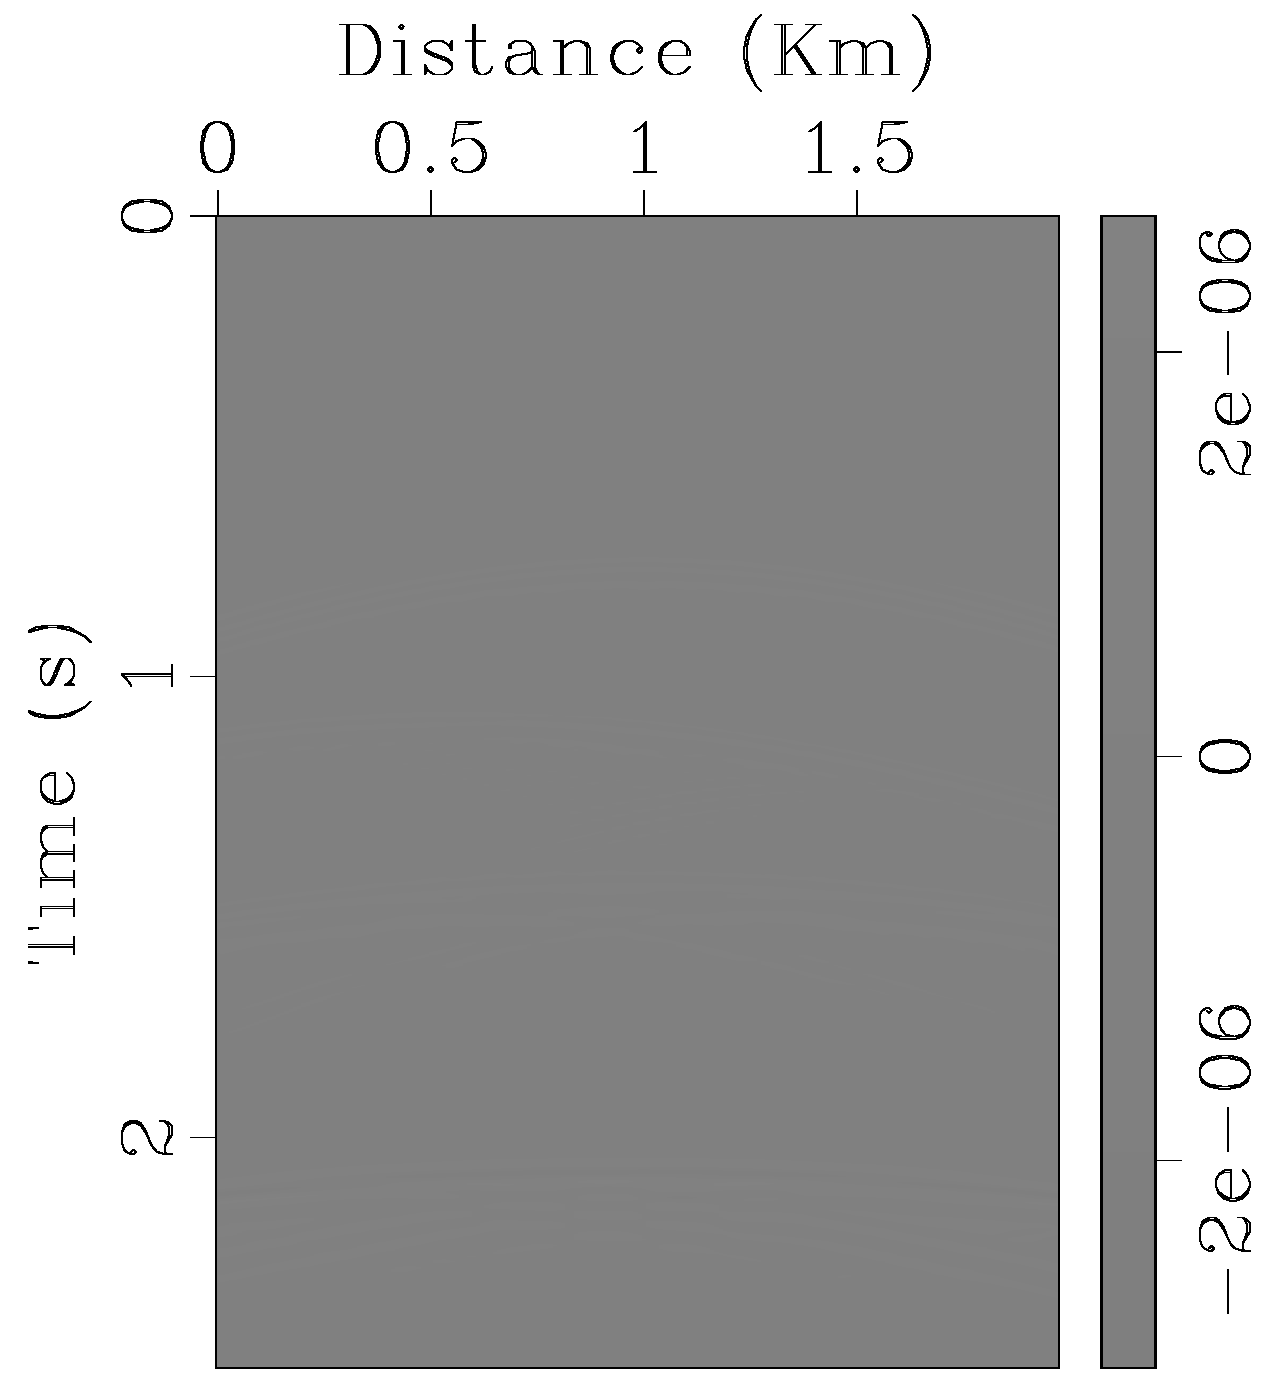
\includegraphics[width=0.47\linewidth]{figure/diff30}}
	\fcaption{数据残差比较:(a)在1km处的单炮记录;(b)跟初始模型正演数据的残差;
	(c)迭代30次后的数据残差。}{(a) The observed data for the shot
	at 1km, (b) the residual with the initial $Q$, and (c) the residual with the 
	$Q$-RWI inverted $Q$.}[数据残差对比结果]
    \label{fig:record_diff}
\end{figure*}

\begin{figure*}[!htbp]
    \centering
	\subfigure[]{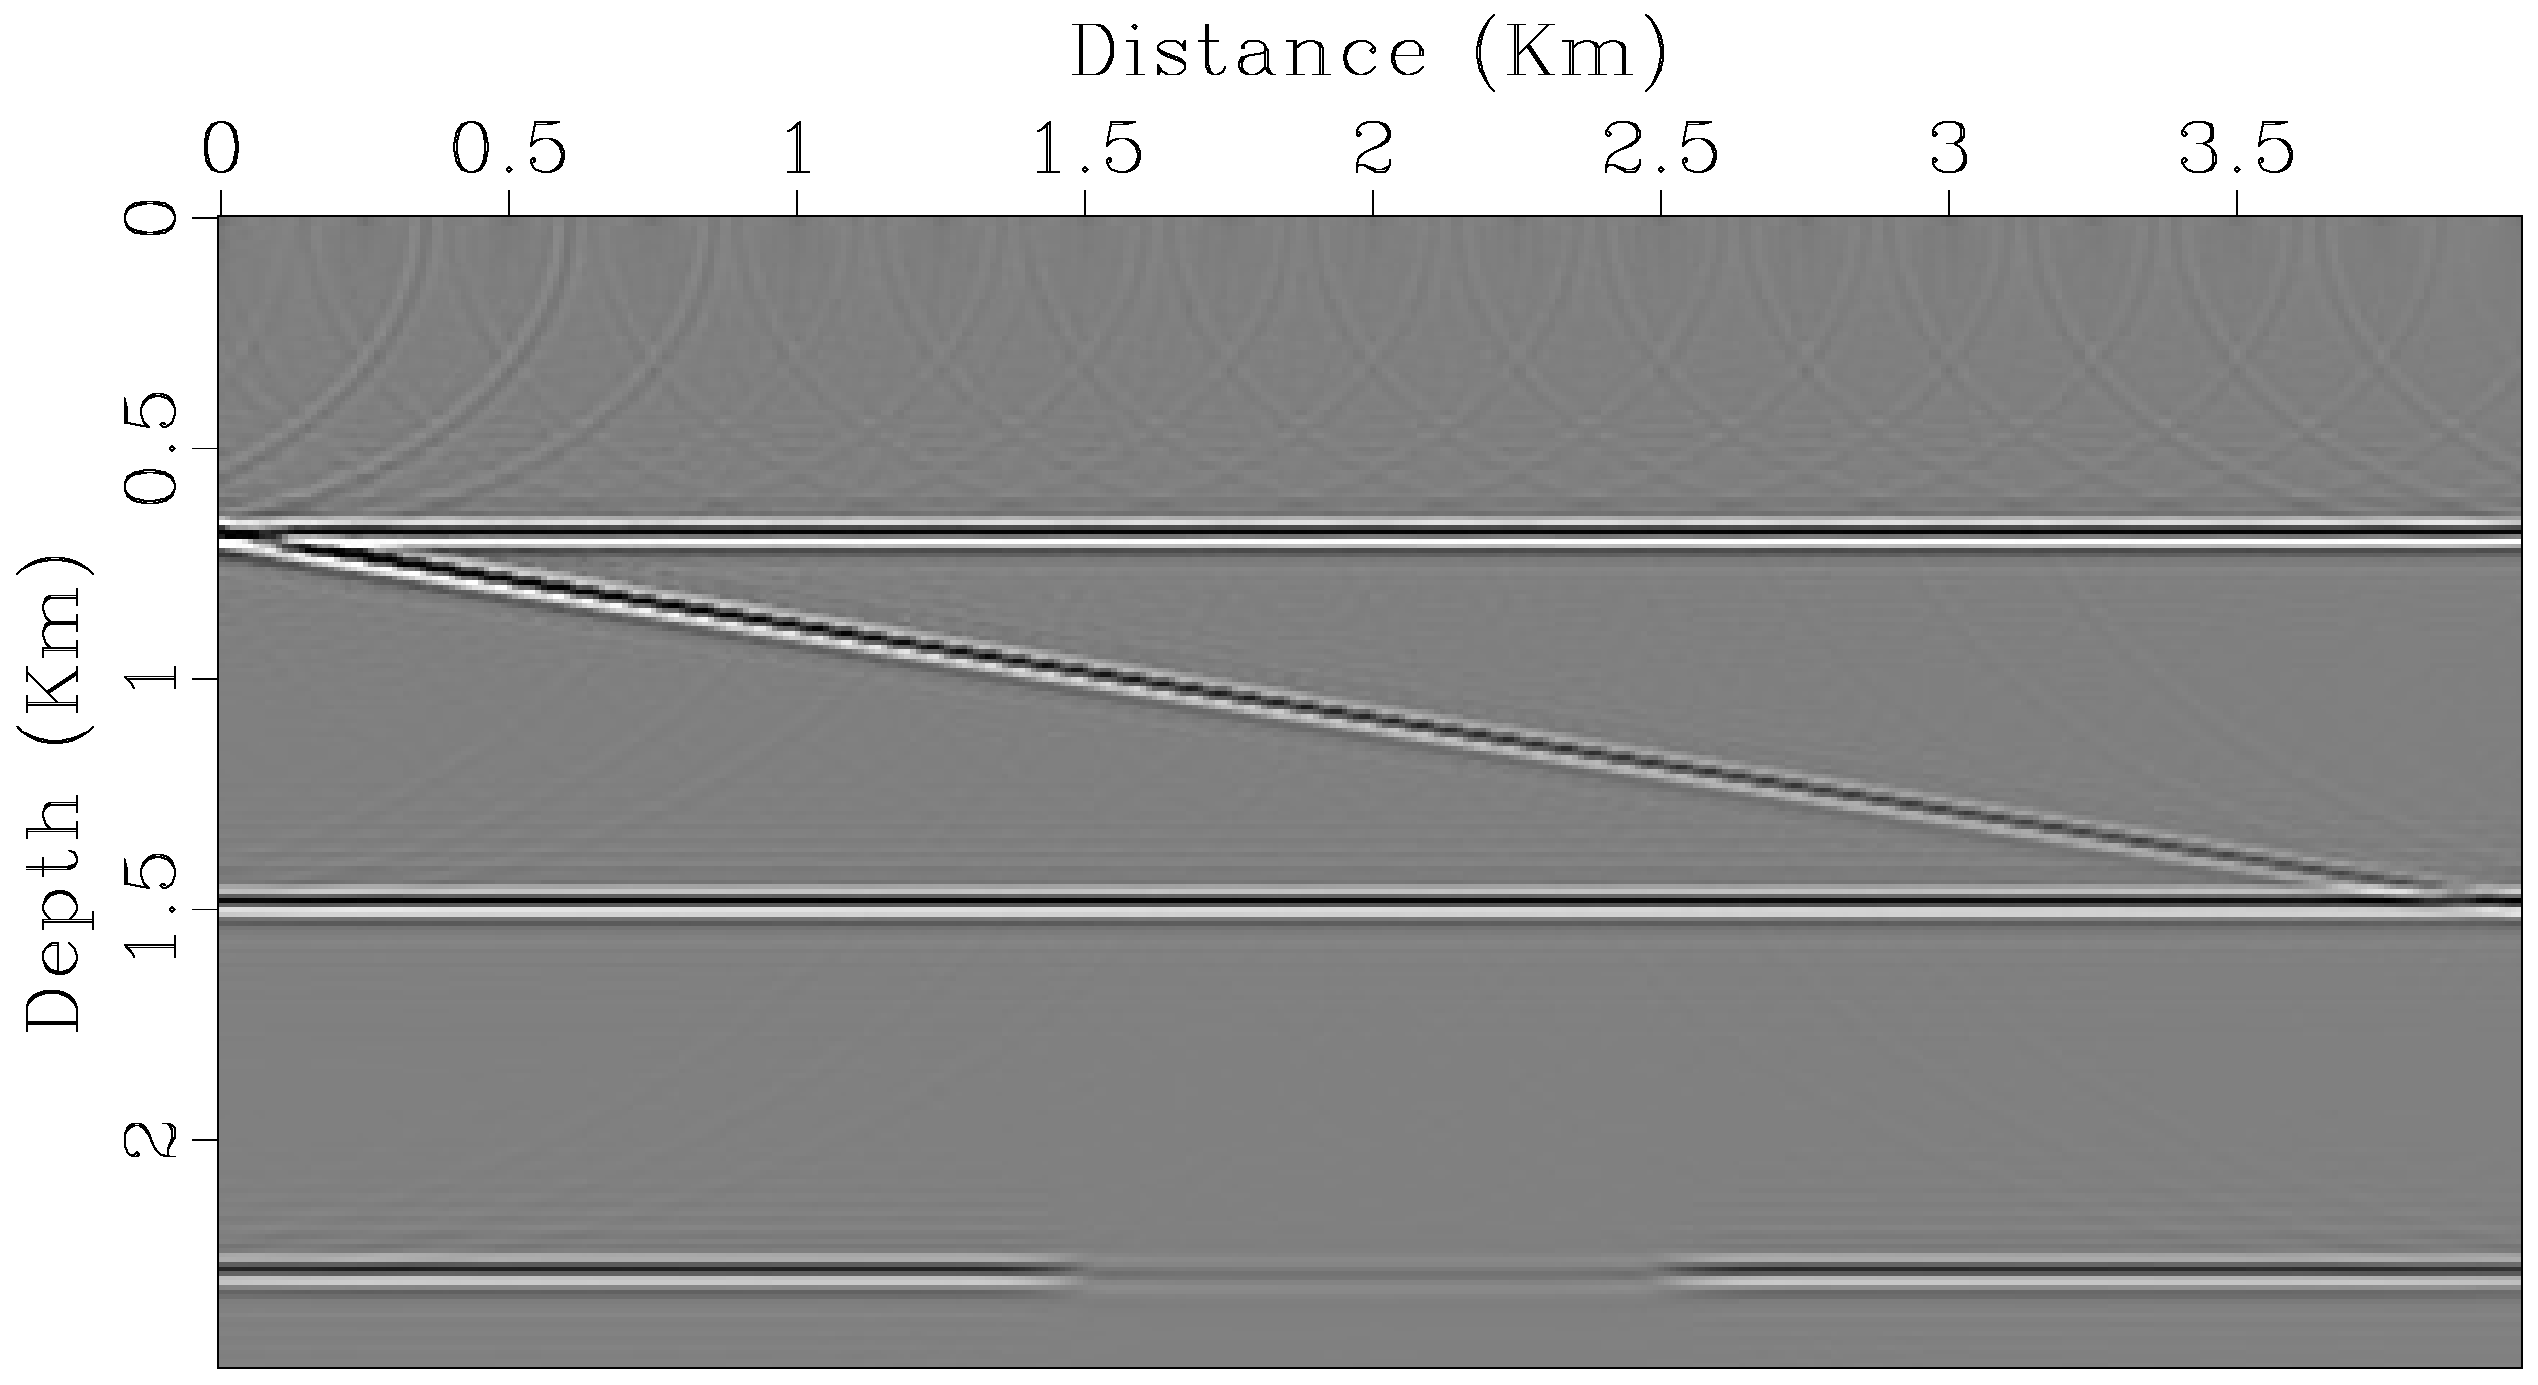
\includegraphics[width=0.72\linewidth]{figure/rtm_no400x250}}
	\subfigure[]{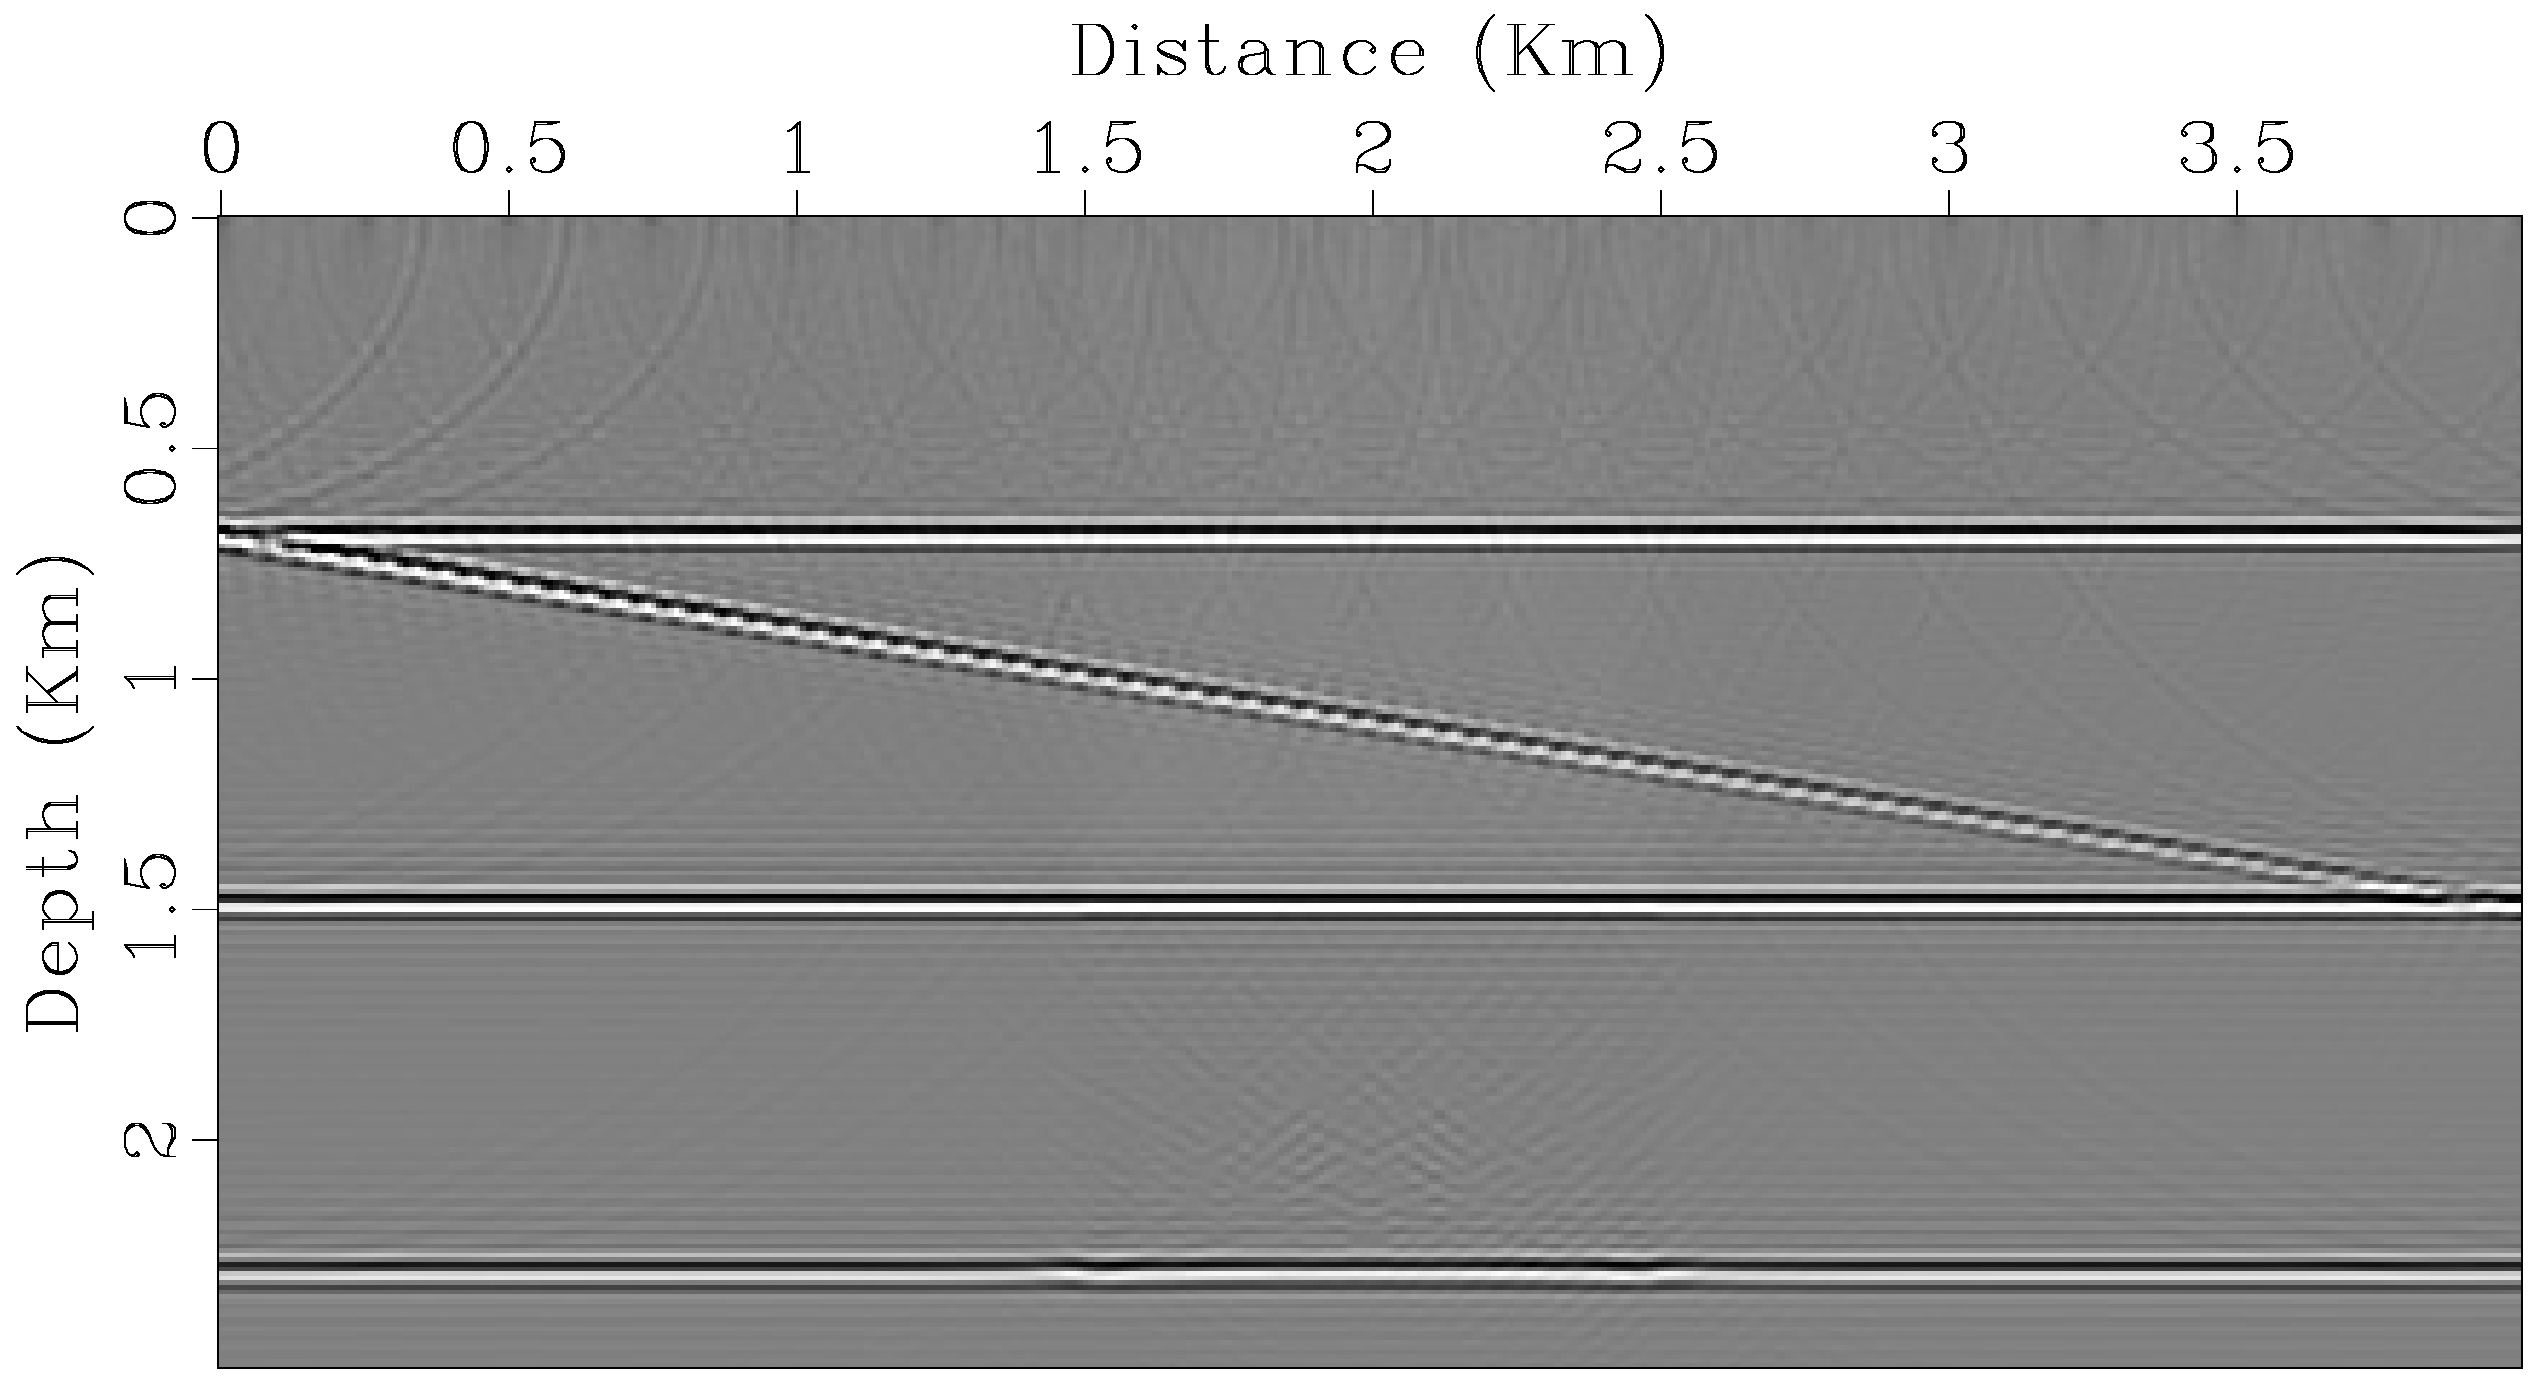
\includegraphics[width=0.72\linewidth]{figure/rtm_true400x250}}
	\subfigure[]{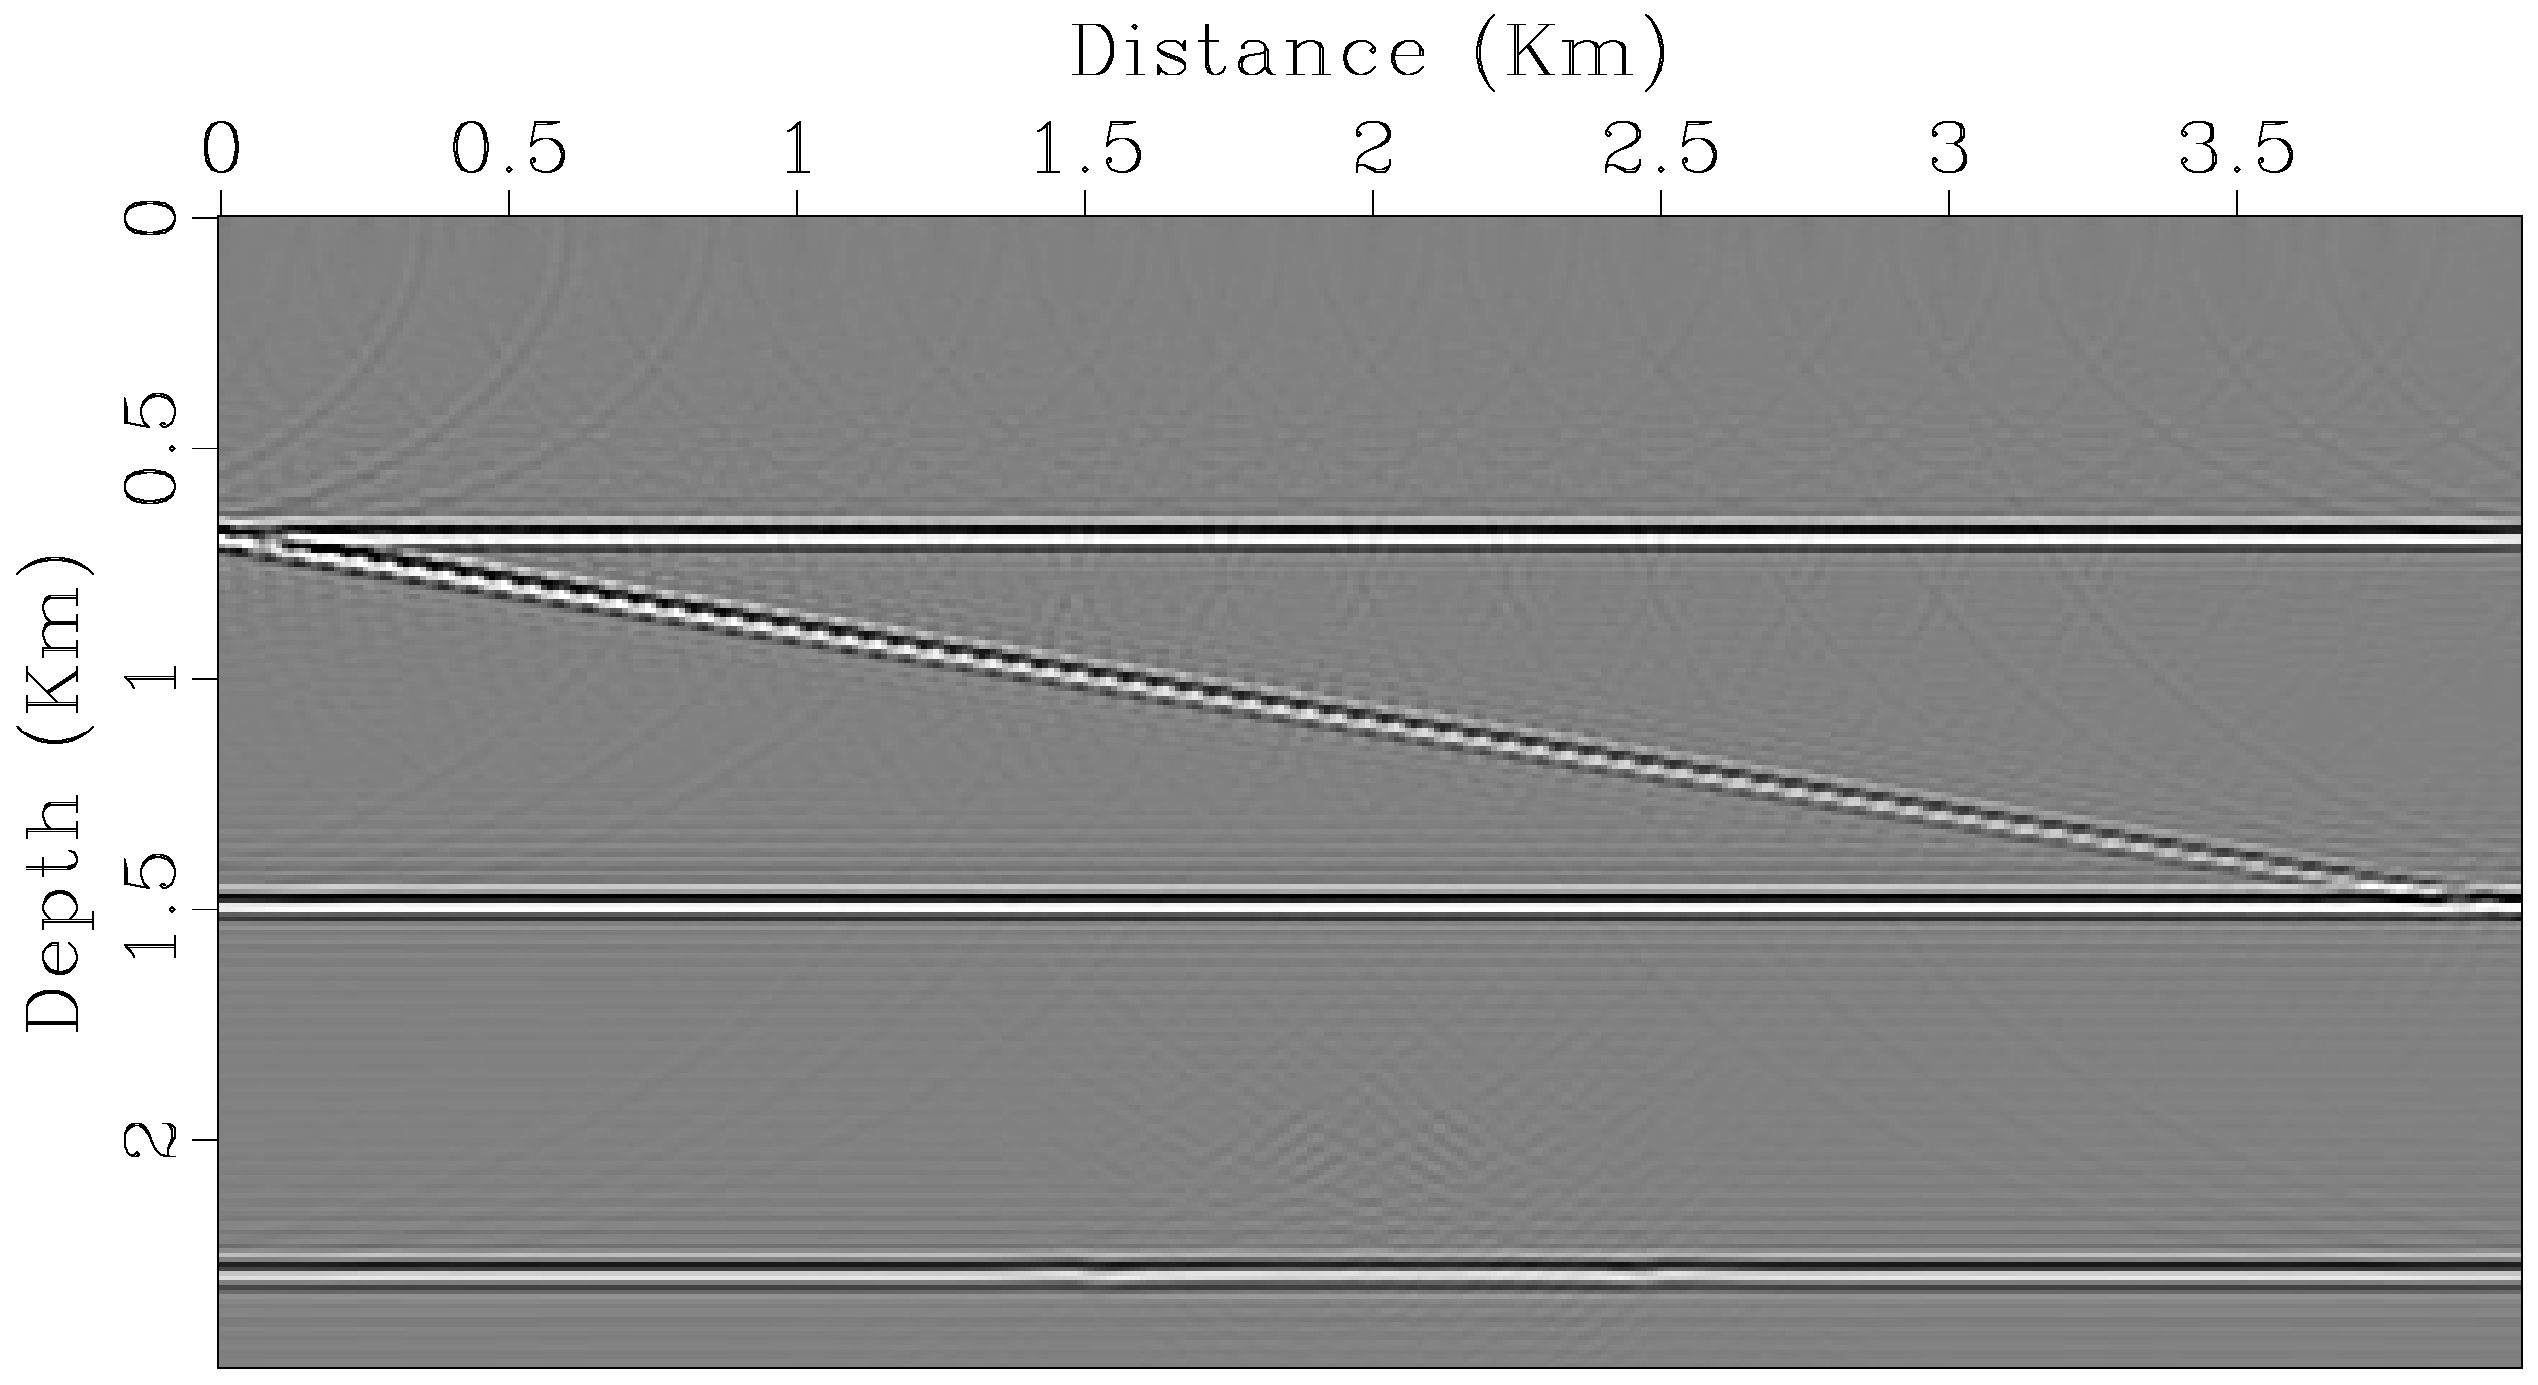
\includegraphics[width=0.72\linewidth]{figure/rtm_fq400x250}}
	\fcaption{$Q$-RTM成像结果:(a)初始$Q$补偿结果;(b)真实$Q$补偿结果;
	$Q$-RWI反演$Q$补偿结果。}{$Q$-compensated RTM images using initial
	$Q$ model (a); true $Q$ model (b) and $Q$-RWI inverted $Q$ model (c).}
	[$Q$-RTM成像结果]
    \label{fig:rtm_model}
\end{figure*}

